\documentclass[bachelor,euler,twoside,openright]{ustcthesis}



\usepackage{listings}
\usepackage{color}
\definecolor{lightgray}{rgb}{.9,.9,.9}
\definecolor{darkgray}{rgb}{.4,.4,.4}
\definecolor{purple}{rgb}{0.65, 0.12, 0.82}

\lstdefinelanguage{JavaScript}{
  keywords={typeof, new, true, false, catch, function, return, null, catch, switch, var, if, in, while, do, else, case, break},
  keywordstyle=\color{blue}\bfseries,
  ndkeywords={class, export, boolean, throw, implements, import, this},
  ndkeywordstyle=\color{darkgray}\bfseries,
  identifierstyle=\color{black},
  sensitive=false,
  comment=[l]{//},
  morecomment=[s]{/*}{*/},
  commentstyle=\color{purple}\ttfamily,
  stringstyle=\color{red}\ttfamily,
  morestring=[b]',
  morestring=[b]"
}

\lstset{
   language=JavaScript,
   backgroundcolor=\color{lightgray},
   extendedchars=true,
   basicstyle=\footnotesize\ttfamily,
   showstringspaces=false,
   showspaces=false,
   numbers=left,
   numberstyle=\footnotesize,
   numbersep=9pt,
   tabsize=2,
   breaklines=true,
   showtabs=false,
   captionpos=b
}




% 默认twoside 双面打印
% 将master修改为bachelor, doctor or master
% 要使用adobe字体,添加adobefonts选项
% 使用euler数学字体,如不愿使用,去掉euler
% 使用外文写作,请添加notchinese

% 设置图形文件的搜索路径
\graphicspath{{figures/}}

\usepackage{enumitem}
\setlist[description]{leftmargin=\parindent,labelindent=\parindent}
%仅用于本示例文档中显示特殊字符串
\usepackage{xltxtra}

%%%%%%%%%%%%%%%%%%%%%%%%%%%%%%
%% 封面部分
%%%%%%%%%%%%%%%%%%%%%%%%%%%%%%

  % 中文封面内容
  \title{面向幼教管理的家长教师社交软件的设计与实现}%一般情况下扉页和封皮、书脊共用一个标题文本,可以不用定义\spinetitle(仅硕博有用), \covertitle(本硕博均有用)和\encovertitle(仅本科有用)。特殊情况见下。
  %\spinetitle{\small{中国科学技术大学本硕博毕业论文模板示例文档\raisebox{-3pt}{(Beta)}}}
  %特殊情况1:本例中\title命令里含有换行控制字符,这会导致制作书脊的时候出现错误,例如如果你注释掉\spinetitle{...}这一行就会报错。这时需要定义一个不含换行等命令的\spinetitle,这并不表示\spinetitle里不能有任何命令——只能使用有限的命令。
  %特殊情况2:本例中标题过长,所以需要缩小书脊标题的字号。
  %特殊情况3:本例中中英文混排,由于tex竖排的原理限制,中英文基线不重合,所以需要人工调整英文的基线。具体调整量根据不同字体有所不同。
  \covertitle{面向幼教管理的家长教师社交软件的设计与实现}
  %\covertitle{中文题目第一行\\中文题目第二行}
  %不要在此调整封皮字体大小! Do not set Cover Page font size here!
  %特殊情况4:本例中\title中含有多个换行,导致标题超过了两行。根据制本厂规定,封皮标题不能超过两行。因此需要定义封皮使用的标题\covertitle. 如果你注释掉这一行,就会发现封皮不符合规定。
  \encovertitle{The Design and Implementation of Social Network Software for the Preschool Education with Management Concern}
  %\encovertitle{English Title Line 1\\English Title Line 2\\English Title Line 3}
  %不要在此调整封皮字体大小! Do not set Cover Page font size here!
  %特殊情况5:仅本科生有用。本科封皮中有英文标题,不超过三行。与上类似。

  \author{张\ 鑫\ 语}
  \depart{信息学院电子工程与信息科学系}%系别,硕博请用系代号,本科请用全称如
  %\depart{数理化和信息工程系}
  %\major{人文管理和生物专业专业}%专业,硕博请用全称,本科不需要
  \advisor{李斌\ 教授}
  %\coadvisor{冯晨珠\ 教授}%第二导师,没有请注释掉
  \studentid{PB11210105}%For bachelor only
  \submitdate{二〇一五年五月}

  % 英文封面内容
  \entitle{The Design and Implementation of Social Network Software for the Preschool Education with Management Concern}
  \enauthor{Xinyu Zhang}
  \enmajor{Department of Electronic Engineering \& Information Science}
  \enadvisor{Prof. Bin Li}
  %\encoadvisor{Prof. Chenzhu Feng}%另外一个导师
  \ensubmitdate{May, 2015}



\begin{document}

  % 封面
  \maketitle

%特别注意,以下述顺序为准,在对应部分添加文档部件,切勿颠倒顺序:
%本科论文的文档部件顺序是:
%    frontmatter:致谢、目录、中文摘要、英文摘要、
%    mainmatter: 正文章节
%    backmatter: 参考文献或资料注释、附录
%硕博论文的文档部件顺序是:
%    frontmatter:中文摘要、英文摘要、目录、符号说明
%    mainmatter: 正文章节
%    backmatter: 参考文献、附录、致谢、发表论文
%%%%%%%%%%%%%%%%%%%%%%%%%%%%%%
%% 前言部分
%%%%%%%%%%%%%%%%%%%%%%%%%%%%%%
\frontmatter
\makeatletter
\ifustc@bachelor
	%%%%%%%%%%%%%%%%%
	%本科论文修改这里
	%%%%%%%%%%%%%%%%%
	% 致谢
	%
\begin{thanks}

感谢原本科模板的作者XPS、硕博模板的作者刘青松以及它们的维护者的辛勤工作!

感谢大家对本模板更新工作的支持!

本模板以及本示例文档还存在许多不足之处,欢迎大家测试并及时提供反馈。

\begin{flushright}
ywg@USTC
\end{flushright}


在中国科技大学完成本科和硕博连读学业的九年里,我所从事的学习和研究工作,都是在导师以及系里其他老师和同学的指导和帮助下进行的。在完成论文之际,请容许我对他们表达诚挚的谢意。

首先感谢导师XXX教授和XXX副教授多年的指导和教诲,是他们把我带到了计算机视觉的研究领域。X老师严谨的研究态度及忘我的工作精神,X老师认真细致的治学态度及宽广的胸怀,都将使我受益终身。

感谢班主任XXX老师和XX老师多年的关怀。感谢XXX、XX、XX等老师,他们本科及研究生阶段的指导给我研究生阶段的研究工作打下了基础。

感谢XX、XXX、XXX、XX、XXX、XXX、XXX、XX等师兄师姐们的指点和照顾;感谢XXX、XX、XXX等几位同班同学,与你们的讨论使我受益良多;感谢XXX、XX、XXX、XX、XXX等师弟师妹,我们在XXX实验室共同学习共同生活,一起走过了这段愉快而难忘的岁月。

感谢科大,感谢一路走过来的兄弟姐妹们,在最宝贵年华里,是你们伴随着我的成长。

最后,感谢我家人一贯的鼓励和支持,你们是我追求学业的坚强后盾。

\vskip 18pt

\begin{flushright}

~~~~赵钱孙~~~~

\today

\end{flushright}

\end{thanks}


	%目录部分
	%目录
	\tableofcontents
	%默认表格、插图、算法索引名称分别为“表格索引”、“插图索引”和“算法索引”
	%如果需要自行修改lot,lof,loa的名称,请定义
	%\ustclotname{...}
	%\ustclofname{...}
	%\ustcloaname{...}

	% 表格索引
	%\ustclot
	% 插图索引
	\ustclof
	%算法索引
	%如果需要使用算法环境并列出算法索引,请加入补充宏包。
	%\ustcloa

	% 摘要
	
\begin{cnabstract}
本文是中国科学技术大学本硕博毕业论文模板示例文件。本模板由ywg@USTC创建,适用于撰写学士、硕士和博士学位论文,本模板由原来的本科模板和硕博模板整合优化而来。本示例文件除了介绍本模板的基础用法外,本文还是一个简要的学位论文写作指南。

\keywords{中国科学技术大学,学位论文,\LaTeX{}~通用模板,学士,硕士,博士}
\end{cnabstract}


\begin{enabstract}

This is USTC thesis template for bachelor, master and doctor user's guide. The template is created by ywg@USTC and a derivative of USTC Bachelor and Master-PhD templates. Besides that
the usage of the template, a brief
guideline for writing thesis is also provided.


\enkeywords{University of Science and Technology of China (USTC), Thesis, Universal \LaTeX{} Template, Bachelor, Master, PhD}
\end{enabstract}
%此文件中含有中英文摘要
\else
	%%%%%%%%%%%%%%%%%
	%硕博论文修改这里
	%%%%%%%%%%%%%%%%%
	% 摘要
	%
\begin{cnabstract}
本文是中国科学技术大学本硕博毕业论文模板示例文件。本模板由ywg@USTC创建,适用于撰写学士、硕士和博士学位论文,本模板由原来的本科模板和硕博模板整合优化而来。本示例文件除了介绍本模板的基础用法外,本文还是一个简要的学位论文写作指南。

\keywords{中国科学技术大学,学位论文,\LaTeX{}~通用模板,学士,硕士,博士}
\end{cnabstract}


\begin{enabstract}

This is USTC thesis template for bachelor, master and doctor user's guide. The template is created by ywg@USTC and a derivative of USTC Bachelor and Master-PhD templates. Besides that
the usage of the template, a brief
guideline for writing thesis is also provided.


\enkeywords{University of Science and Technology of China (USTC), Thesis, Universal \LaTeX{} Template, Bachelor, Master, PhD}
\end{enabstract}
%此文件中含有中英文摘要
	% 目录
	\tableofcontents
	%默认表格、插图、算法索引名称分别为“表格索引”、“插图索引”和“算法索引”
	%如果需要自行修改lot,lof,loa的名称,请定义
	%\ustclotname{...}
	%\ustclofname{...}
	%\ustcloaname{...}

	% 表格索引
	\ustclot
	% 插图索引
	\ustclof
	%算法索引
	%如果需要使用算法环境并列出算法索引,请加入补充宏包。
	\ustcloa

	%符号说明,需要加入补充包
	%\begin{denotation}

\item[HPC] 高性能计算 (High Performance Computing)
\item[cluster] 集群
\item[Itanium] 安腾
\item[SMP] 对称多处理
\item[API] 应用程序编程接口
\item[PI]	聚酰亚胺
\item[MPI]	聚酰亚胺模型化合物,N-苯基邻苯酰亚胺
\item[PBI]	聚苯并咪唑
\item[MPBI]	聚苯并咪唑模型化合物,N-苯基苯并咪唑
\item[PY]	聚吡咙
\item[PMDA-BDA]	均苯四酸二酐与联苯四胺合成的聚吡咙薄膜
\item[$\Delta G$]  	活化自由能~(Activation Free Energy)
\item [$\chi$] 传输系数~(Transmission Coefficient)
\item[$E$] 能量
\item[$m$] 质量
\item[$c$] 光速
\item[$P$] 概率
\item[$T$] 时间
\item[$v$] 速度
\end{denotation}
%不是必需的,如果不想列出请注释掉
\fi
\makeatother

%%%%%%%%%%%%%%%%%%%%%%%%%%%%%%
%% 正文部分
%%%%%%%%%%%%%%%%%%%%%%%%%%%%%%
\mainmatter

  \chapter{绪论}

\section{研究背景和意义}

该项目属于产品型而并非research, 意在设计一种产品, 以App和PC Web端的形式来满足幼儿教育领域的用户需求.   



当下随着互联网 Online To Offline 大潮的愈演愈烈,人们的日益增长的需求,互联网, 移动计算,办公, 服务社交化极大地改变了人们生活的方式, 并且让市场愈发细化, 出现了大量特定领域的应用和软件。 而这里设计并实现的一款产品, 是为了满足幼教领域中不同人群的各种需求:


\begin{itemize}
	\item 幼儿园管理层
	\item 幼儿园教师
	\item 宝宝家长
\end{itemize}


需求列表可以简单地概括为:

\begin{itemize}
	\item 幼儿园老师和家长之间交互
	\item  幼儿园管理层对于老师的有效管理
	\item 家长对于自己孩子生活点滴的记录
	\item 家长之间针对孩子的社交
\end{itemize}

该软件能够让幼儿园的管理更加轻松, 家长与老师和其他家长的联系更加紧密, 对于孩子的爱护更加贴心到位。


\section{国内外发展现状}

国内针对幼教母婴的类似软件已经存在, 比如:

\begin{figure}[H]
	\centering
	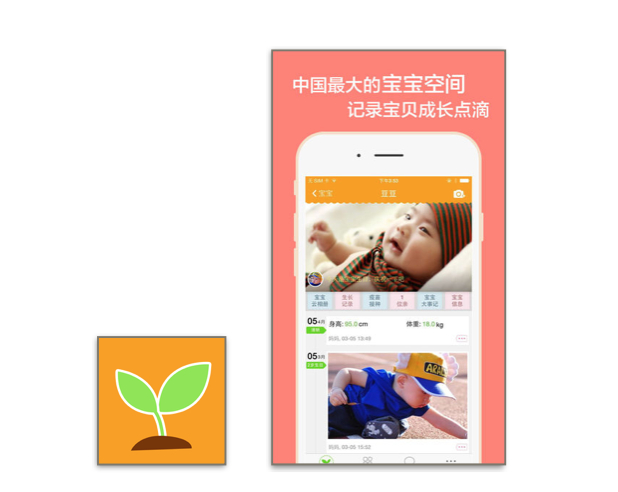
\includegraphics[width=0.80\textwidth]{qbb.png}
	\figcaption{亲宝宝}
	\label{fig:qinbaobao}
\end{figure}

亲宝宝是一个针对家长设计的app, 让亲友能够方便地记录宝宝的成长记录, 并且有一定的分享功能。

\begin{figure}[H]
	\centering
	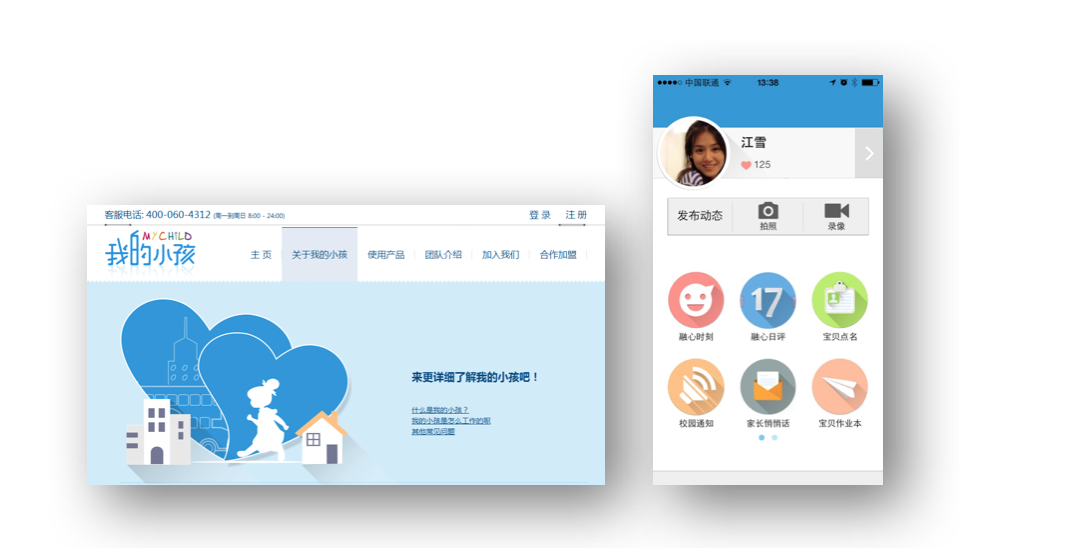
\includegraphics[width=0.80\textwidth]{hhz.png}
	\figcaption{好孩子}
	\label{fig:haohaizi}
\end{figure}

好孩子是一个面向幼儿园的人员管理系统, 有一定的社交功能, 但社交功能不强, 而且因为产品设计问题, 现在已经从itunes中下架, 而且只支持iphone端。



现在大部分幼儿园并没有对于人员的管理的信息系统, 老师和家长之间的交流方式主要通过微信,短信, QQ群。  


\section{课题主要内容与工作}

需要实现一个Web端, Web端的功能主要是管理, 面向用户为幼儿园管理层和幼儿园教师, 管理层主要功能:
	
	\begin{itemize}
		\item 	班级管理
		\begin{itemize}
			\item 班级中文件, 相册
			\item 班级中人员的转班, 入学
			\item 教师给父母发送学生的教师评语
			\item 班级中人员的转班, 入学
			\item 发布班级通知
		\end{itemize}
		
			\item 学校管理
		\begin{itemize}
			\item 学校中文件, 相册
			\item 学校中班级的管理
			\item 发布学校通知
		\end{itemize}
		 
		\item 不同教师拥有不同的权限
	
	\end{itemize}


在管理端的基础上, 实现App端, App端的功能主要是社交,老师, 管理者, 家长都会参与其中, 社交的主要功能有:

\begin{itemize}
	\item 每个用户都可以发布时间线
	\item 每个用户在自己主页看到同班用户发的时间线
	\item 可以在每个学校主页看到这个学校所有人发的时间线
	\item 可以提出加入班级申请
\end{itemize}


\section{论文结构}

在第一章, 我大致讲解了该产品的应用背景, 简述了应当具有的功能,在第二章, 我会介绍该产品使用到的技术和原则, 第三章, 我会进行详尽的需求分析。第四章, 会给出系统的概要设计。 在第五章, 详细介绍系统的设计与实现细节。第六章会大致讲解系统的测试, 最后第七章给出该项目的总结和展望。


  \chapter{相关技术与知识}


\section{经典EIM系统总体介绍}

EIM系统的英文全称是 Enterprise Information Management System.  在这个应用中需要首先实现一个适合幼儿园的学生教师人员管理的信息系统, 作为整个系统的数据基础。




一个EPM系统一般使用关系型数据库, 提供Web接口, 让不同用户登录, 同时操作。 并且还需要有一定程度上的权限管理机制。  在当下市场中, 有很多现成的商业化EPM系统, 为公司提供General的解决方案。 


\begin{figure}[H]
	\centering
	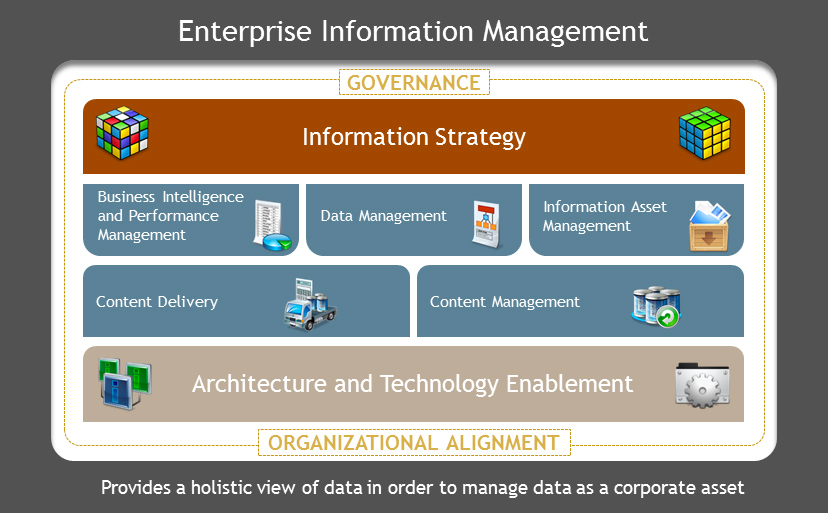
\includegraphics[width=0.80\textwidth]{eim.png}
	\figcaption{Enterprise Information Management System}
	\label{fig: Enterprise Information Management System}
\end{figure}


但这些系统的问题往往是

\begin{itemize}
\item 不领域相关, 而幼儿园有十分独特的人员管理需求
\item 提供了大量不必要的功能
\item 因为功能太多, 也造成使用昂贵
\item 不能加以扩展, 比如支持社交
\end{itemize}

\section{社交SNS类型软件总体介绍}



社交SNS软件是互联网浪潮的一大标志, 它满足了人们的聊天,分享,交友的需求。在这个应用中, 基于管理端的数据, 在老师和家长中做班级为单位的的社交, 所以要实现一个适合该应用场景的社交App.




一般一个社交SNS软件的扩展性, 速度, 及时性十分重要, 而原子性并不强求。 所以大多使用非关系型数据库, 往往都会提供手机App, 不一定提供Web PC应用。在当下市场中, 有很多社交软件, General的社交软件最出名的是 Facebook


\begin{figure}[H]
	\centering
	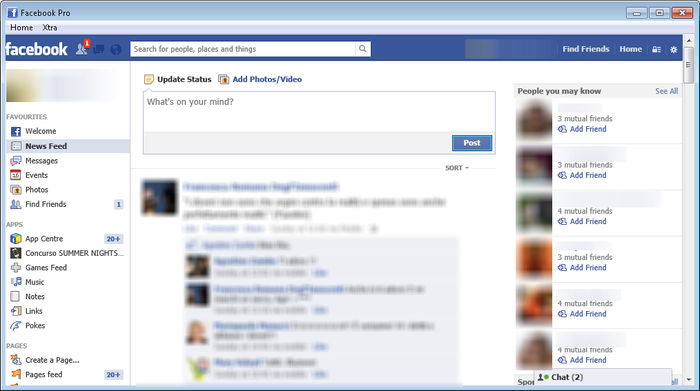
\includegraphics[width=0.80\textwidth]{fb.png}
	\figcaption{facebook}
	\label{fig: fb}
\end{figure}


而对于细分的市场, 各种软件百花齐放。


微信,基于熟人社交

\begin{figure}[H]
	\centering
	
\includegraphics[width=0.80\textwidth]{wechat.png}
	\figcaption{微信}
	\label{fig: wechat}
\end{figure}

陌陌,基于陌生人社交


\begin{figure}[H]
	\centering
	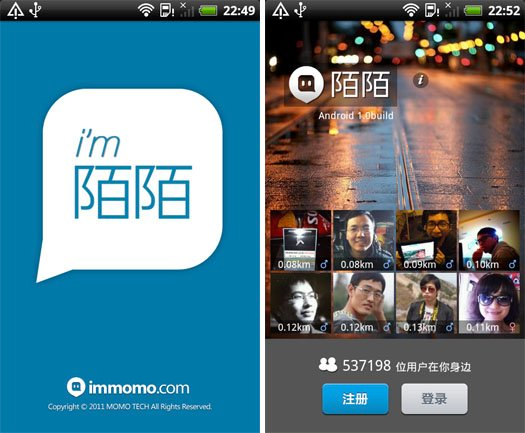
\includegraphics[width=0.80\textwidth]{momo.png}
	\figcaption{陌陌}
	\label{fig: momo}
\end{figure}

Airbnb, 基于租房社交

\begin{figure}[H]
	\centering
	
\includegraphics[width=0.80\textwidth]{airbnb.png}
	\figcaption{airbnb}
	\label{fig: airbnb}
\end{figure}


Spotify, 音乐社交, 基于Facebook

\begin{figure}[H]
	\centering
	
\includegraphics[width=0.80\textwidth]{spotify.png}
	\figcaption{Spotify}
	\label{fig: spotify}
\end{figure}


在这里, 要实现的社交是基于细分的幼儿教育市场。


\section{基于EPM管理系统的社交软件相关技术简介}

对于该应用, 由于要加入社交元素, 加之人员管理系统只需要针对幼教领域来设计功能, 所以使用了非关系型数据库mongodb。 


在Web后端使用了Nodejs来进行程序开发, web前端操作逻辑比较复杂, 所以使用了angularjs前端框架。因为前后端交互比较频繁, 大量使用了websocket而不是Http Ajax访问来进行前后端交互。



App的开发往往比较费时, 尤其是考虑到如何跨平台。 在这里我选用了 Hybrid Html5 Mobile开发框架, 可以使用Web技术来开发 ios \& android 平台app, 一份代码, 两个平台使用。而且Web技术也降低了开发门槛和学习曲线。


\subsection{Nosql 简介}


\begin{figure}[H]
	\centering
	
\includegraphics[width=0.80\textwidth]{nosql.png}
	\figcaption{Nosql}
	\label{fig: nosql}
\end{figure}

NoSQL有时也称作Not Only SQL的缩写,是对不同于传统的关联式数据库的数据库管理系统的统称。(注依据Martin Fowler,NoSQL 不是英文Not Only SQL, 因为这会是NOSQL 而不是NoSQL)



两者存在许多显著的不同点,其中最重要的是NoSQL不使用SQL作为查询语言。其数据存储可以不需要固定的表格模式,也经常会避免使用SQL的JOIN操作,一般有水平可扩展性的特征。NoSQL的实现具有二个特征:使用硬盘,或者把随机存储器作存储载体。



当代典型的关联式数据库在一些数据敏感的应用中表现了糟糕的性能,例如为巨量文档建立索引、高流量网站的网页服务,以及发送流式媒体关系型数据库的典型实现主要被调整用于执行规模小而读写频繁,或者大批量极少写访问的事务。



NoSQL的结构通常提供弱一致性的保证,如最终一致性,或交易仅限于单个的数据项。不过,有些系统,提供完整的ACID保证在某些情况​​下,增加了补充中间件层(例如,CloudTPS。有两个成熟的系统有提供快照隔离的列存储:像是Google基于过滤器系统的BigTable,和滑铁卢大学发展的HBase。这些系统,自主开发,使用类似的概念来实现多行(multi-row)分散式ACID交易的快照隔离(snapshot isolation)保证为基础列储存,无需额外的资料管理开销,中间件系统部署或维护,减少了中间件层。



少数NoSQL系统部署了分布式结构,通常使用分散式杂凑表(DHT)将数据以冗余方式保存在多台服务器上。依此,扩充系统时候添加服务器更容易,并且扩大了对服务器失效的承受能程度


\subsection{Mongodb 简介}

\begin{figure}[H]
	\centering
	
\includegraphics[width=0.80\textwidth]{mongo.png}
	\figcaption{mongodb}
	\label{fig: mongo}
\end{figure}


	是由C++语言编写的开源数据库系统。 在高负载的情况下,添加更多的节点,可以保证服务器性能。MongoDB 旨在为WEB应用提供可扩展的高性能数据存储解决方案。
	
	
	
	MongoDB是一种强大、灵活、追求性能、易扩展的数据存储方式。是面向文档的数据库,不是关系型数据库,是NoSQL(not only SQL)的一种。所谓的面向文档,就是将原来关系型数据库中的“行”的概念换成了更加灵活的”文档",以文档为存储单位。文档的值可以是数组、文档等复杂的数据模型。并且文档的键不会事先定义也不会固定不变。mongoDB设计的主要思想之一就是,将能交给客户端的操作都要从服务端转移到客户端,例如生成objectid等操作。
	
	

\subsection{Nodejs 简介}

\begin{figure}[H]
	\centering
	
\includegraphics[width=0.80\textwidth]{node.png}
	\figcaption{Node}
	\label{fig: node}
\end{figure}


Node.js是一个基于Chrome JavaScript运行时建立的平台, 用于方便地搭建响应速度快、易于扩展的网络应用。Node.js 使用事件驱动, 非阻塞I/O 模型而得以轻量和高效,非常适合在分布式设备上运行的数据密集型的实时应用。


V8引擎执行Javascript的速度非常快,性能非常好。

Node是一个Javascript运行环境(runtime)。实际上它是对Google V8引擎进行了封装。V8引 擎执行Javascript的速度非常快,性能非常好。Node对一些特殊用例进行了优化,提供了替代的API,使得V8在非浏览器环境下运行得更好。

\subsection{Angularjs 简介}

\begin{figure}[H]
	\centering
	
\includegraphics[width=0.80\textwidth]{ng.png}
	\figcaption{angular}
	\label{fig: angular}
\end{figure}

AngularJS是一款开源JavaScript函式库,由Google维护,用来协助单一页面应用程序运行的。它的目标是透过MVC模式(MVC)功能增强基于浏览器的应用,使开发和测试变得更加容易。

函式库读取包含附加自定义(标签属性)的HTML,遵从这些自定义属性中的指令,并将页面中的输入或输出与由JavaScript变量表示的模型绑定起来。这些JavaScript变量的值可以手工设置,或者从静态或动态JSON资源中获取。

\subsection{Hybrid HTML5 Mobile App 简介}

\begin{figure}[H]
	\centering
	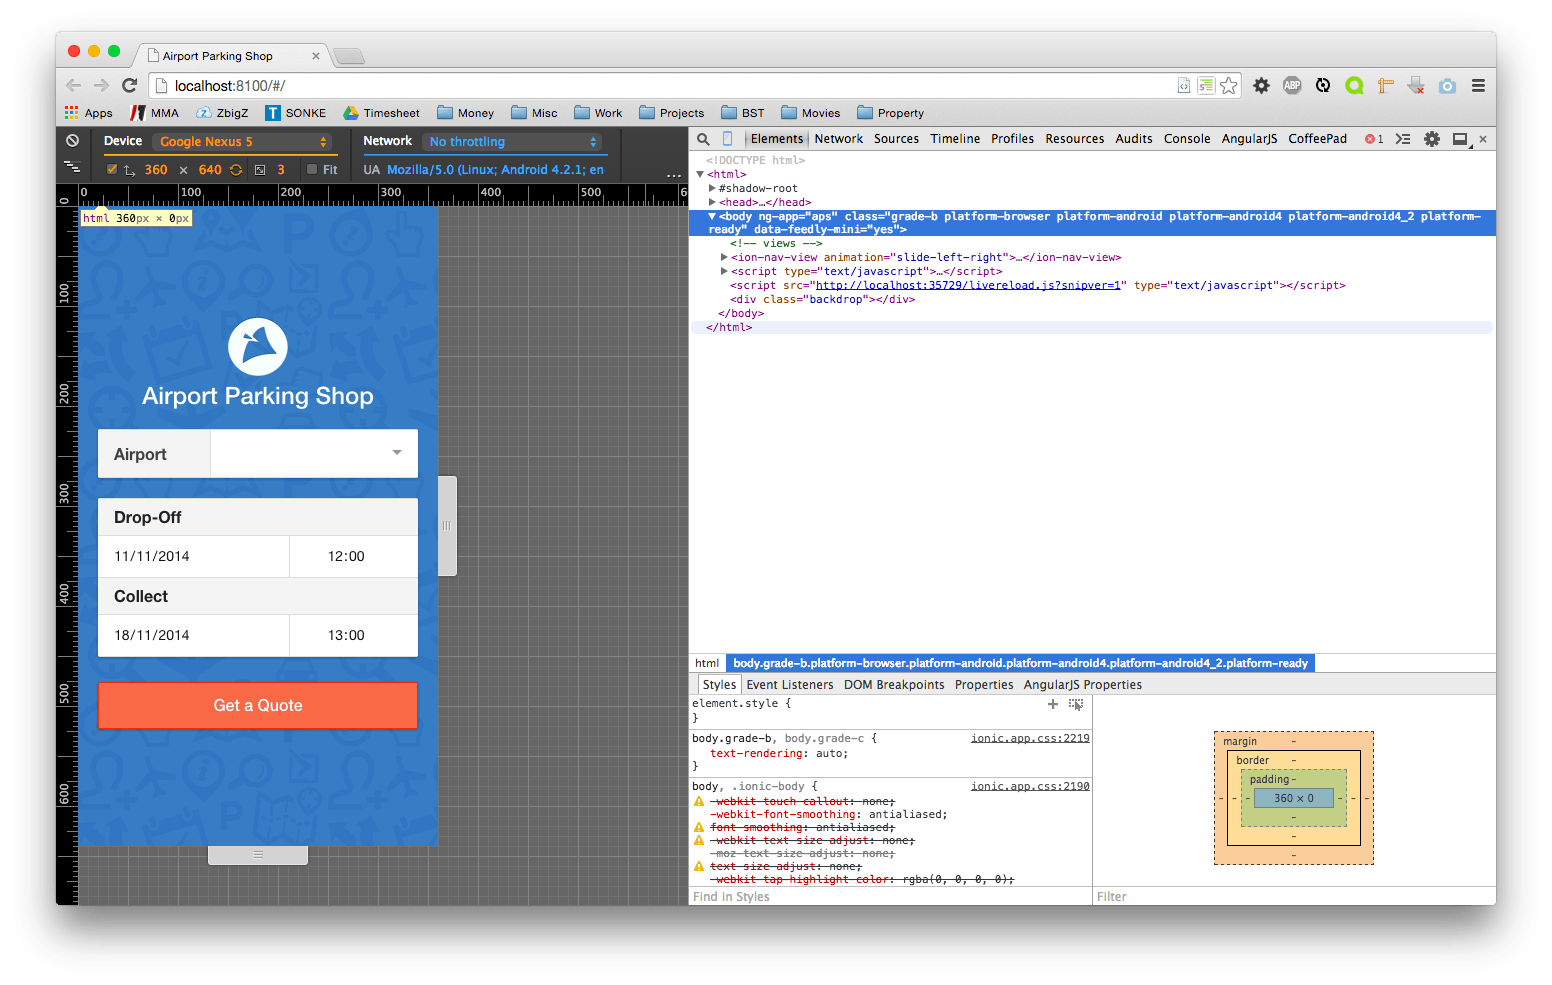
\includegraphics[width=0.80\textwidth]{ionic.png}
	\figcaption{Hybrid App Dev}
	\label{fig: had}
\end{figure}



Hybrid App是指介于web-app、native-app这两者之间的app,它虽然看上去是一个Native App,但只有一个UI WebView,里面访问的是一个Web App,但其通过JSB (javascript Binding)来和系统底层的api交流, 来达到native app的功能, 但却可以使用Web 技术来渲染UI。

另一种方式是使用虚拟的HTML DOM, 把Html Dom来翻译为系统的UI布局代码, 来达到原生应用的UI渲染效率。

现有有很多Html5混合手机开发框架, React Native, ionic等等, 我选用了ionic.


\subsection{WebSocket 简介}

\begin{figure}[H]
	\centering
	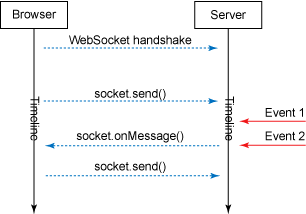
\includegraphics[width=0.80\textwidth]{websocket.png}
	\figcaption{websocket}
	\label{fig: websocket}
\end{figure}

WebSocket是HTML5开始提供的一种在单个 TCP 连接上进行全双工通讯的协议。WebSocket通信协议于2011年被IETF定为标准RFC 6455,WebSocketAPI被W3C定为标准。

在WebSocket API中,浏览器和服务器只需要做一个握手的动作,然后,浏览器和服务器之间就形成了一条快速通道。两者之间就直接可以数据互相传送。
  \chapter{系统需求分析}

\section{ 管理端功能性需求分析}

\subsection{所有功能}

管理端面对两种用户, 分别为幼儿园管理者和教师, 他们分别有不同的需求。 下面首先分析 幼儿园管理者角色所要求的功能:

\begin{itemize}

\item 注册/登录

\item 将自己的幼儿园录入系统

\begin{itemize}
	\item 幼儿园创建
	\item 删除
	\item 编辑相关信息
\end{itemize}


\item 幼儿园有自己的
\begin{itemize}
	\item 相册
	\begin{itemize}
		\item 上传
		\item 修改图片名和介绍
	\end{itemize}
	\item 云文件
	\begin{itemize}
		\item 上传
		\item 修改名字和介绍
	 	\item 创建文件夹
		\item 移动文件
	\end{itemize}
\end{itemize}


\item 发布校园通知

\item 在幼儿园录入系统后,在每个隶属于自己的幼儿园名下录入班级
\begin{itemize}
	\item 创建班级
	\item 删除
	\item 编辑相关信息
\end{itemize}

\item 每个班级都有自己的
\begin{itemize}
	\item 相册
	\item 云文件
\end{itemize}


\item 发布班级通知

\item 班级内部的人员管理

\begin{itemize}
	\item 邀请教师/学生
	\item 删除教师
	\item 教师转班
	\item 申请删除学生
	\item 申请学生转班
\end{itemize}


\item 对学生写评语

\item 如果班级和学生数量比较大, 则少数的管理者不可能承担这么多的工作, 而且管理者本身不愿意也不应当干学生数据修改等底层操作

\begin{itemize}
	\item 委派帮手
	\item 以给予手下教师不同权限的形式
	\item 比如有的教师可以做班级内的人员管理, 有的教师允许发布校园通知	
\end{itemize}
	
\end{itemize}

以上是管理者所拥有的功能, 事实上也是该系统PC管理端要提供的全部功能, 因为管理者权限最高, 应当能够使用到全部的功能。



对于教师, 分为基本功能和权限下功能。 基本功能所有教师都有, 权限下每个功能只有管理者分配了权限, 才可以拥有。

\subsection{教师基本功能}

\begin{itemize}
	\item 管理自己所在班级的
	\begin{itemize}
		\item 相册
		\item 班级文件
	\end{itemize}
	\item 发布自己所在班级通知
	\item 对自己班级内的学生写评语
\end{itemize}



\subsection{教师权限控制功能}

\begin{itemize}
	\item 校园层级上的功能
	\begin{itemize}
		\item 发布幼儿园通知
		\item 修改幼儿园基本信息 
	\end{itemize}
	   
	
	\item 班级层级上的功能
	
	\begin{itemize}
		\item 	创建班级
		\item  删除班级
		\item  编辑相关信息
	\end{itemize}
\end{itemize}



\section{社交端功能性需求分析}


社交端功能体现在手机App上, 没有用户的权限之说。 下面对社交端所需的功能做一个列表。


\begin{itemize}
	\item 不提供好友功能
	
	\item 用户自动被分入相应班级的聊天群
	
	\item 班级/学校有时间轴, 由其中父母和教师发布的状态组成
	
	\item 发布状态,可以是文字,图片或者是视频
	
	\item 看到同班 (可选为同校) 的其他父母发的状态,并且评论或者点赞
	
	\item 每个用户发布的状态会同步到该用户所在的班级和学校
	
	\item 查看
	\begin{itemize}
		\item 学校通知
		\item 班级通知
		\item 教师评语
	\end{itemize}
	
	
	\item 浏览自己孩子所在班级和学校的
	
	\begin{itemize}
		\item 相册
		\item 文件
	\end{itemize}
		
	\item 私信聊天功能
\end{itemize}


\section{业务流程需求分析}
业务流由下面的业务流图说明:

\newpage
l \newline
\begin{figure}[H]
	\centering
	\hspace*{-7cm}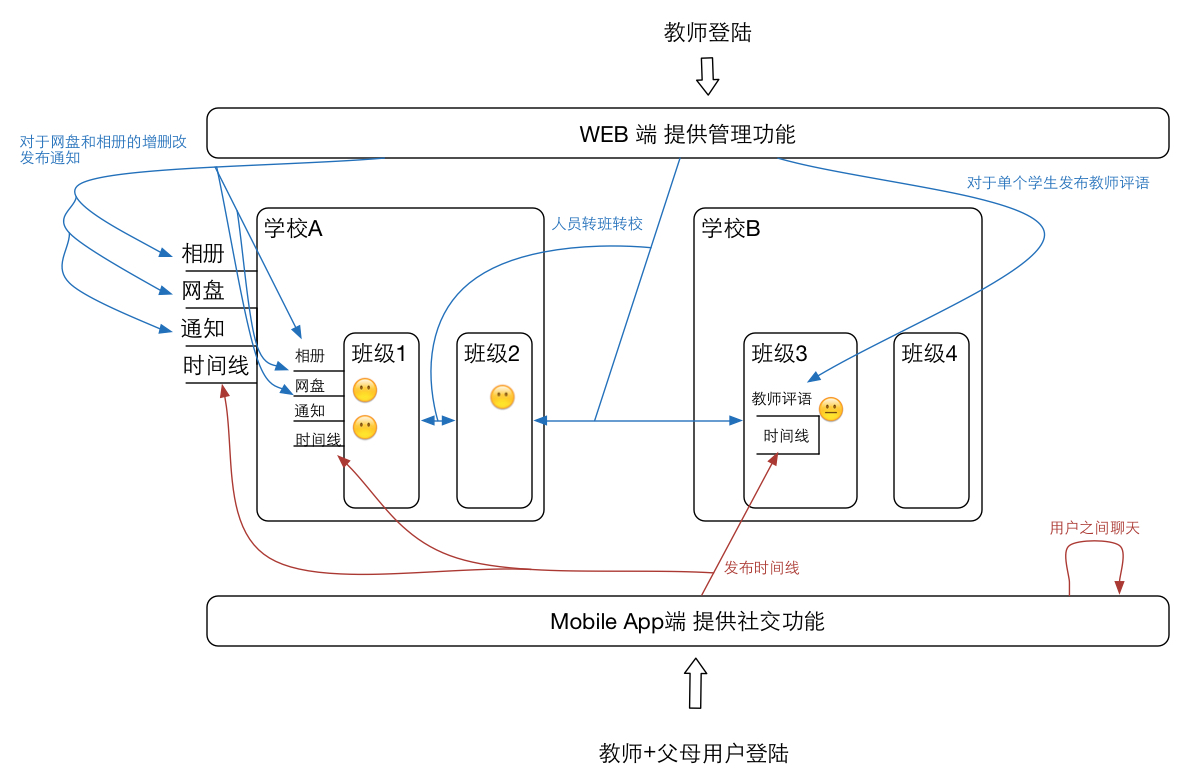
\includegraphics[width=\textwidth]{need-find.jpg}
	\figcaption{业务流图}
	\label{fig:need-find}
\end{figure}


业务流程为, 教师通过Web端登陆进行

\begin{itemize}
	\item 对于幼儿园数据的管理
	\item 发布通知
	\item 给父母发送教师评语
\end{itemize}

 父母和教师用户都可以从Mobile App端登陆
\begin{itemize}
	\item 以班级为单位的群聊
	\item 私信
	\item 发布时间线
	\item 用户的时间线可以同步在其所在的学校, 班级
\end{itemize}

\section{ 非功能性需求分析}

用户有一些非功能性的需求,下面列出来

\begin{itemize}
	

\item 保护学生用户(也就是父母)的权利

\begin{itemize}
	\item 转班,入学,从班级中删除等操作必须要通过父母的短信验证
	\item 如果是父母自行从班级中撤出, 不需要验证
\end{itemize}



\item 管理者账号有权加入任何班级群


\item 对于教师账号, 为了方便管理端的操作

\begin{itemize}
	\item 教师加入某个班级需要教师短信验证
	\item 而对于教师转班,从班级中撤出操作, 可以管理者直接操作, 不需要验证
\end{itemize}

\end{itemize}
  \chapter{系统概要设计}

\section{技术方案介绍}


该应用在服务器端采用Node.js编写, 其好处是Web开发生态环境好, 现成的服务和工具多, 在这里我使用npm提供的 private node modules和github提供的付费 organization 的服务, 将整个大程序设计为由分成多个Node.js的模块组成。



\section{数据库架构设计}


下面

根据我们之前给的需求图, 我们设计出了我们的 mongodb数据库 架构。 见下图:

\newpage
l \newline
\begin{figure}[H]
	\centering
        \hspace*{-7cm}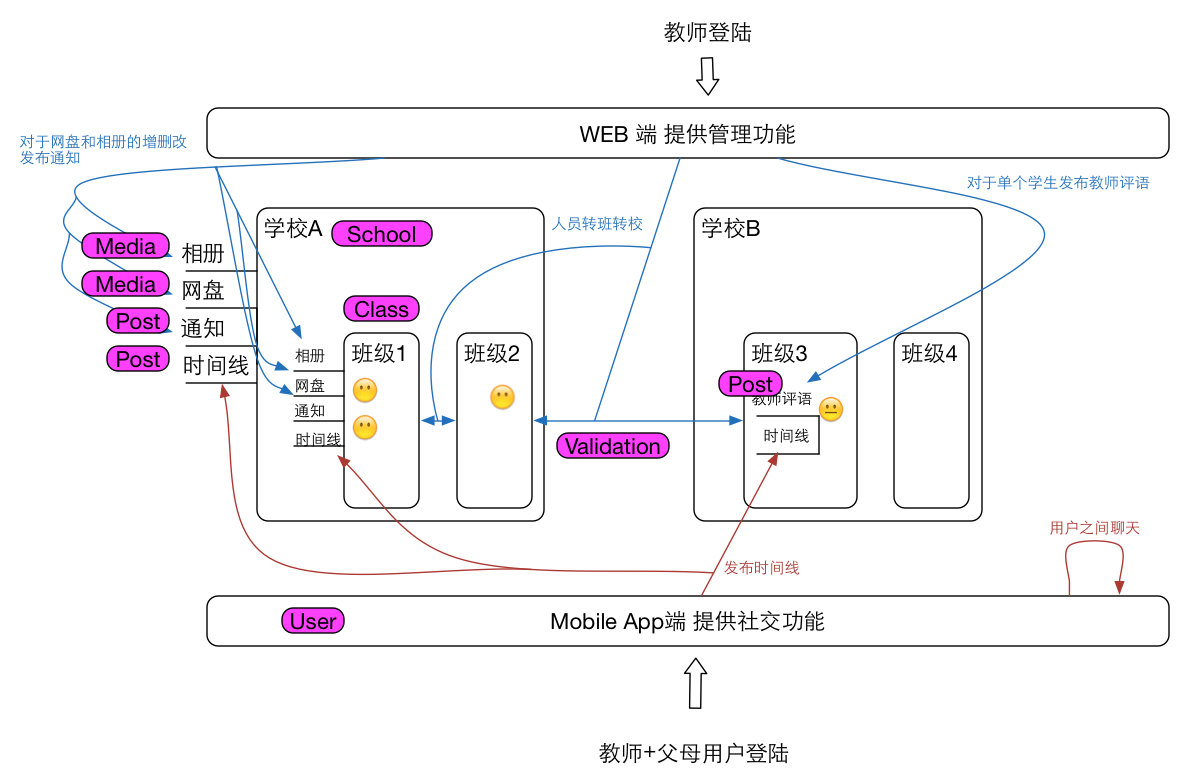
\includegraphics[width=\textwidth]{need-find-db.jpg}
	\figcaption{由业务流图而来的数据库设计}
	\label{fig:need-find-db}
\end{figure}

由上图可见, 其中紫色矩形部分为数据库中定义的model, 分别为:


\begin{description}
	\item[Post]  \hfill \\
	\thinspace 用户发布在时间线的状态
		\item[User]  \hfill \\
		\thinspace 用户模型
		\item[School]  \hfill \\
		\thinspace 学校模型
			\item[Class]  \hfill \\
			\thinspace 班级模型
			\item[Media]  \hfill \\
			\thinspace 文件模型, 用于网盘和相册
	\item[ValidationToken]  \hfill \\
	\thinspace 验证Token, 用于转班验证, 密码reset等

\end{description}


\section{系统后端功能架构设计}


\subsection{思路}

在系统后端, 我运行了两个服务器, 一个是普通的http服务器, 另一个是websocket服务器。 Http 服务器来处理普通的http请求, 并提供一些restful的接口。 websocket服务器和WEB端的管理用户建立socket连接, 实现双向的通信, 以达到

\begin{itemize}
	\item 更加安全
	\item 比ajax http请求更加快捷,高效
\end{itemize}





而这两个服务器提供的功能由一些node modules组成。 首先先要设计程序由哪些部分组成, 之后将这些部分设计为node modules。

\subsection{系统模块架构}

这里先给出 node modules的树形关系图, modules之间关系的设计借鉴了 java 中package命名空间的规范。 在给出关系图后, 会讲解每个module的功能, 和应当暴露出来的接口。node modules 树形关系图类似java程序的类图。

\newpage
\begin{figure}[H]
	\centering
	\vspace*{7cm}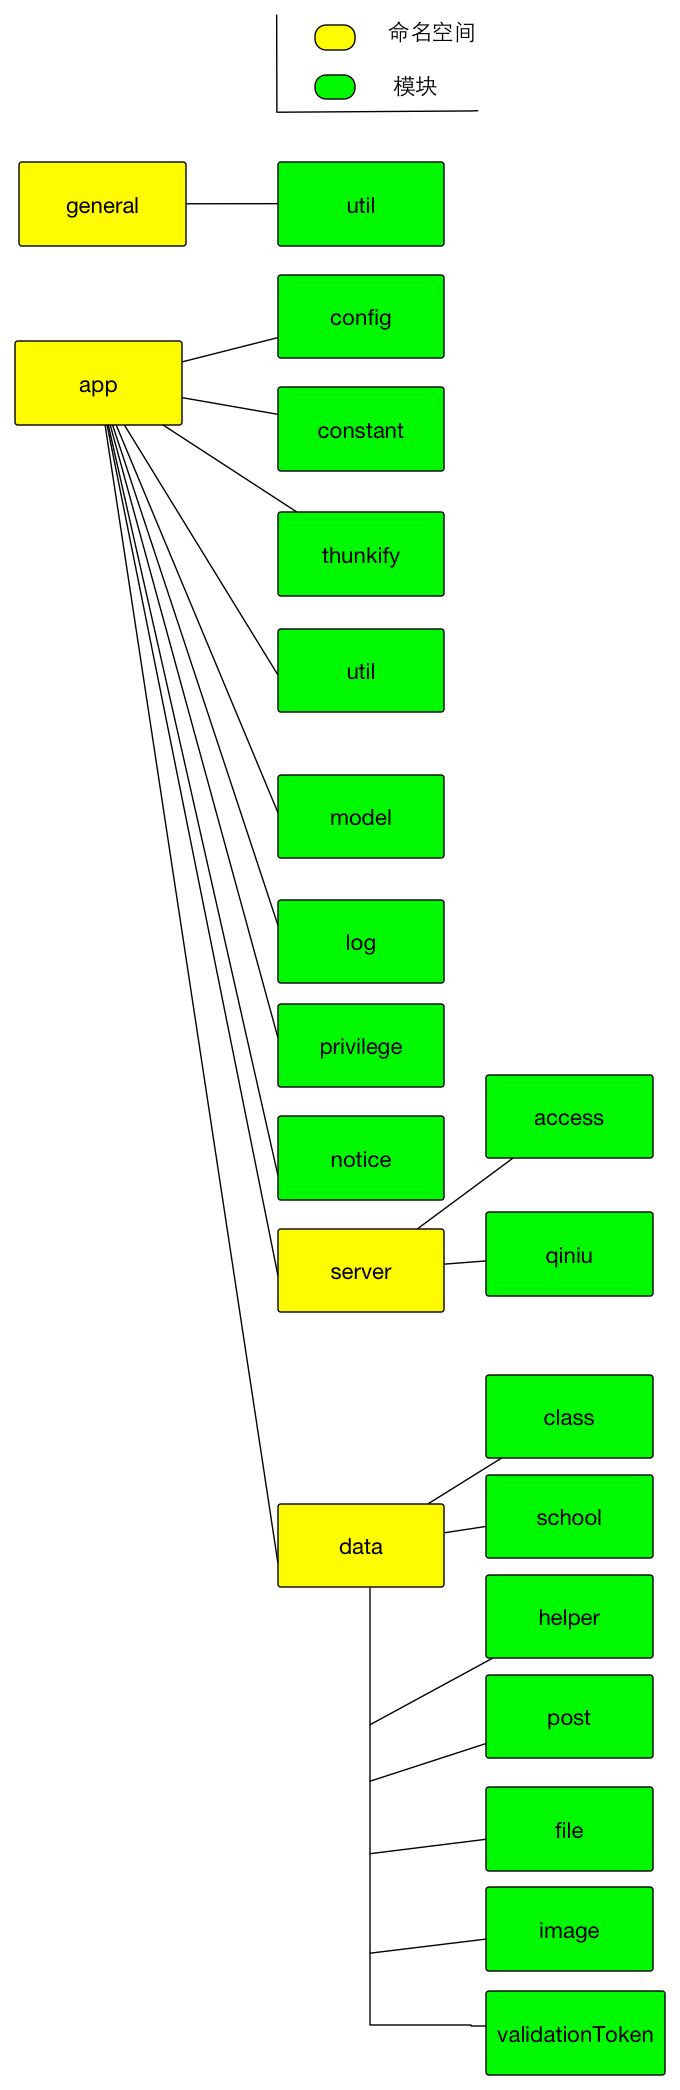
\includegraphics[width=0.35\textwidth]{modules_tree.jpg}
	\figcaption{Node 模块关系}
	\label{fig: modules}
\end{figure}

\newpage
\subsection{系统每个模块作用}

\begin{description}
	\item[general.util] 放一些任何地方都可能被重用到,且与该应用关系不大的代码
	\item[app.config]  配置信息
	\item[app.constant] 使用的一些常量
	\item[app.model] 数据库定义
	\item[app.thunkify]   数据库的一个浅层包装, 对数据库部分操作提供promise形式的接口

	\item[app.util] 一些很多地方都可能被重用到,但与该应用场景耦合度较高的代码
	
	\item[app.log] 日志系统
	
	\item[app.notice] 发短信,邮件,手机端Push Notification通知系统
	
	\item[app.privilege] 系统对于权限相关的操作
	
	\item[app.server.access] 系统服务器的验证(登陆,注册)系统
	
	\item[app.server.qiniu] 系统使用的七牛云服务操作
	
	\item[app.data.class] 对于数据库中班级的抽象层
	
	\item[app.data.school] 对于数据库中学校的抽象层
	
	\item[app.data.helper] 对于数据库中帮手的抽象层
	
	\item[app.data.file] 对于数据库中文件的抽象层
	
	\item[app.data.image] 对于数据库中相册的抽象层
	
	\item[app.data.validationToken] 对于数据库中验证的抽象层
	
	
\end{description}



\subsection{系统模块设计要点}


\begin{enumerate}
	\item 要保证这些modules直接高内聚, 低耦合,直接互相依赖度低, 都可以被当做独立的工具使用
	\item 使用 Github organization, 每个modules都对应organization中的一个 repository. 
	\item 将每个repository都发布为私有的 NPM 模块, 这样可以在任何地方使用 npm install 来进行模块的安装, 使得该应用的每个部分都成为独立的工具
	
	\item 最上层的程序应当很短,只是调用相应模块, 创建服务器并将模块注入其中, 之后服务器开始运行
	
\end{enumerate}













  \chapter{系统详细设计与实现}

\section{数据库架构设计}

下面我给出数据库的详细设计, 因为使用的是nosql, 所以并没有sql经典的设计表, 而是结构化的数据定义

\subsection{用户}

\begin{figure}[H]
	\centering
        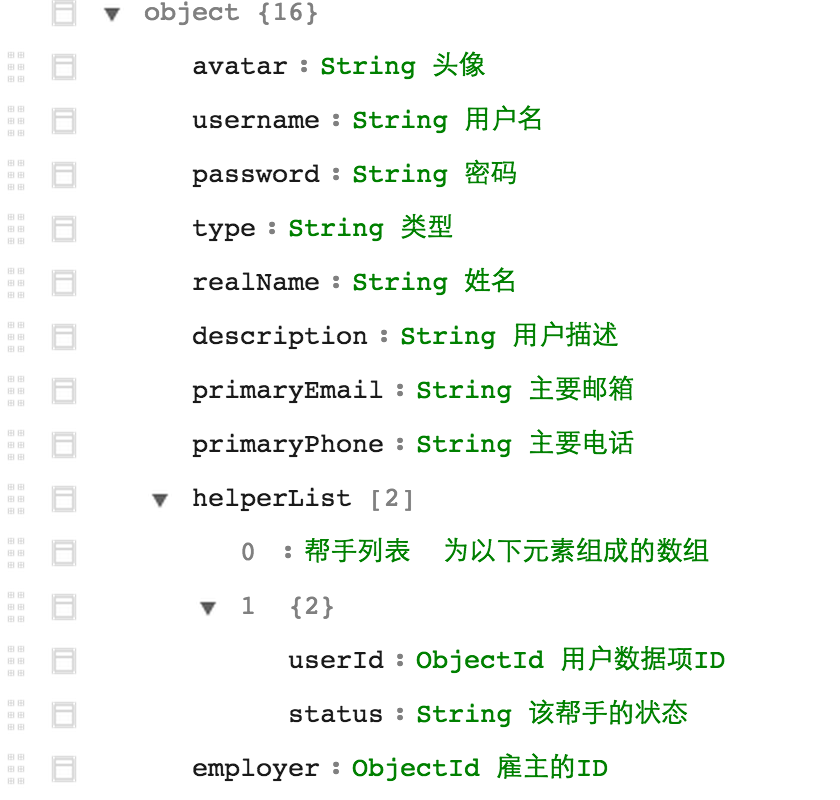
\includegraphics[width=0.45\textwidth]{user-1.png}
        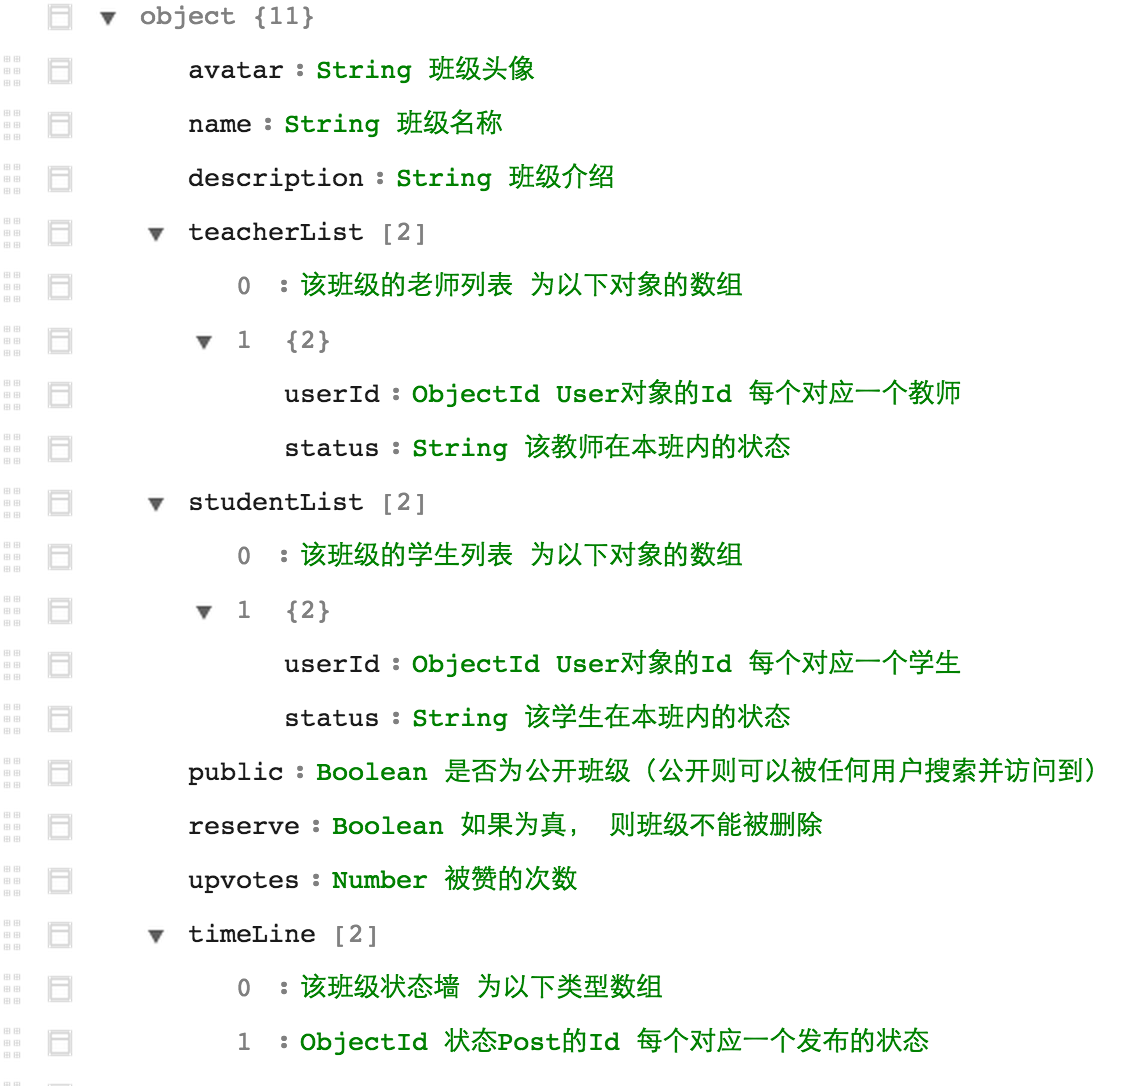
\includegraphics[width=0.45\textwidth]{user-2.png}
        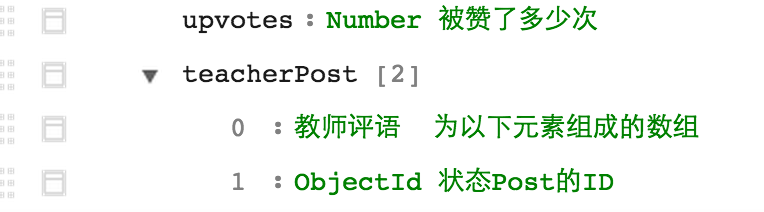
\includegraphics[width=0.45\textwidth]{user-3.png}
	\figcaption{用户模型具体定义}
	\label{fig:user-defined}
\end{figure}


\subsection{学校}


\begin{figure}[H]
	\centering
        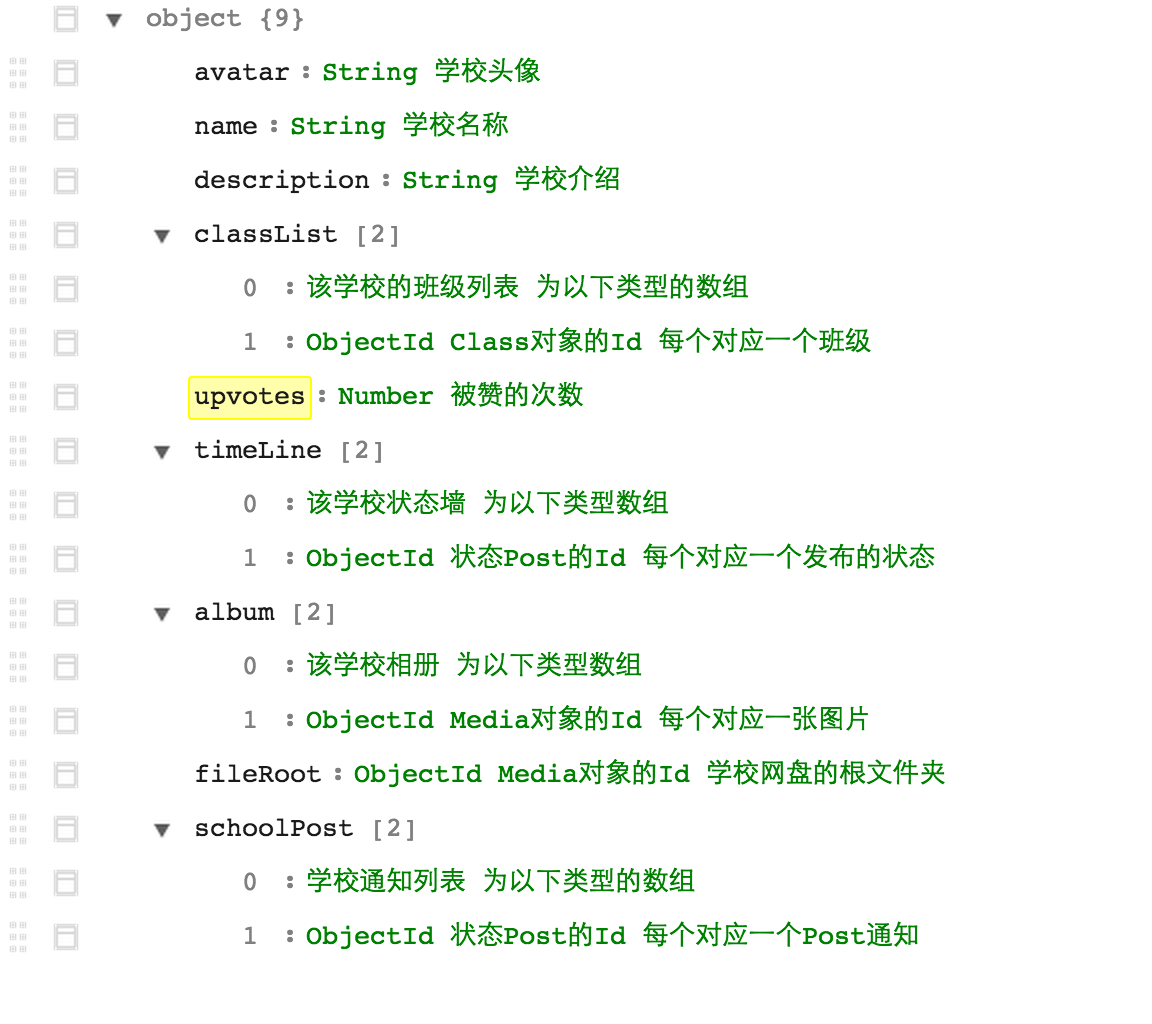
\includegraphics[width=0.8\textwidth]{school.png}
	\figcaption{学校模型具体定义}
	\label{fig:school-defined}
\end{figure}

\subsection{班级}

\begin{figure}[H]
	\centering
        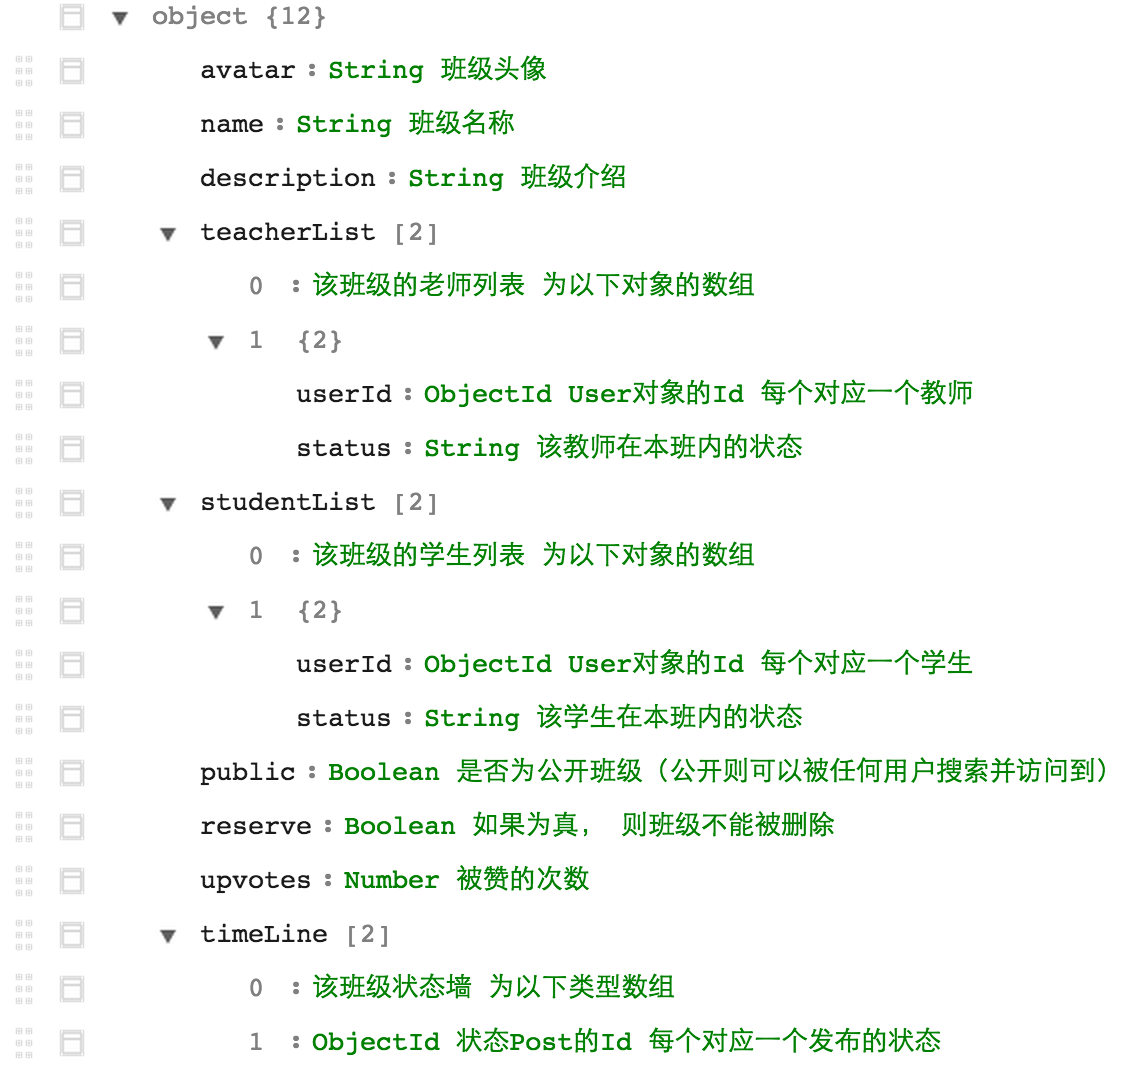
\includegraphics[width=0.45\textwidth]{class-1.png}
        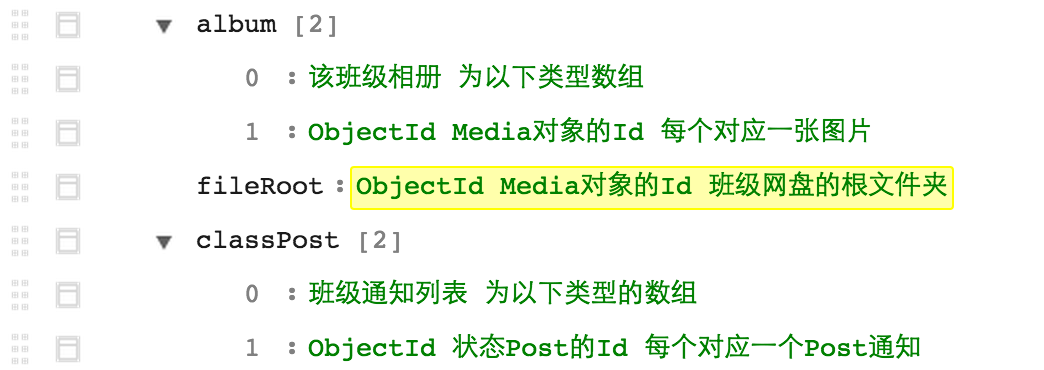
\includegraphics[width=0.45\textwidth]{class-2.png}
	\figcaption{班级模型具体定义}
	\label{fig:class-defined}
\end{figure}

\subsection{状态}

\begin{figure}[H]
	\centering
        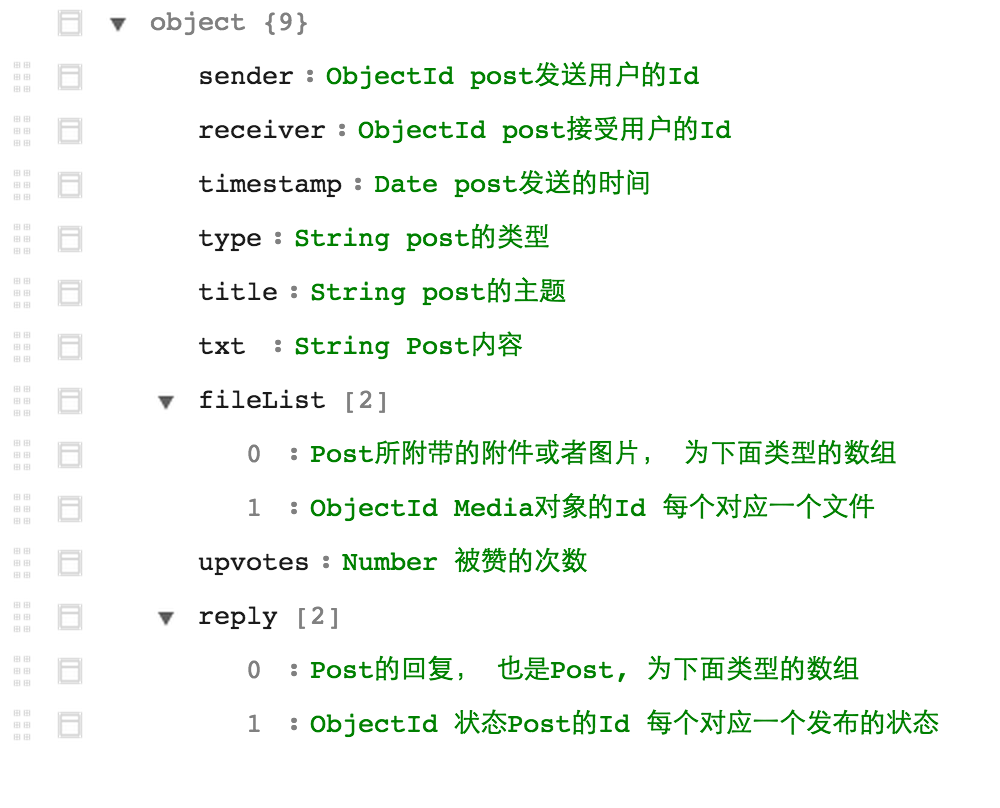
\includegraphics[width=0.8\textwidth]{post.png}
	\figcaption{状态模型具体定义}
	\label{fig:post-defined}
\end{figure}

\subsection{媒体Media (文件的存储)}

\begin{figure}[H]
	\centering
        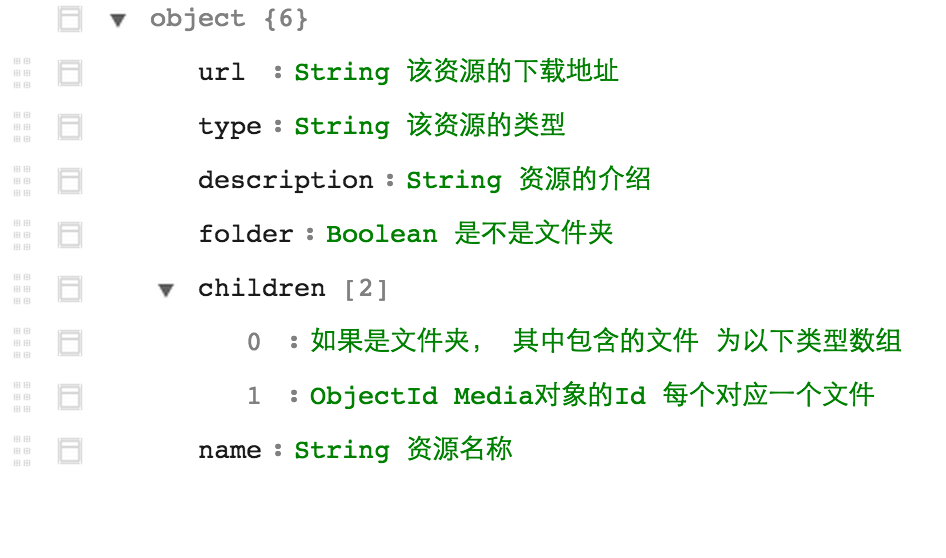
\includegraphics[width=0.8\textwidth]{media.png}
	\figcaption{文件模型具体定义}
	\label{fig:media-defined}
\end{figure}

\subsection{验证Token}

\begin{figure}[H]
	\centering
        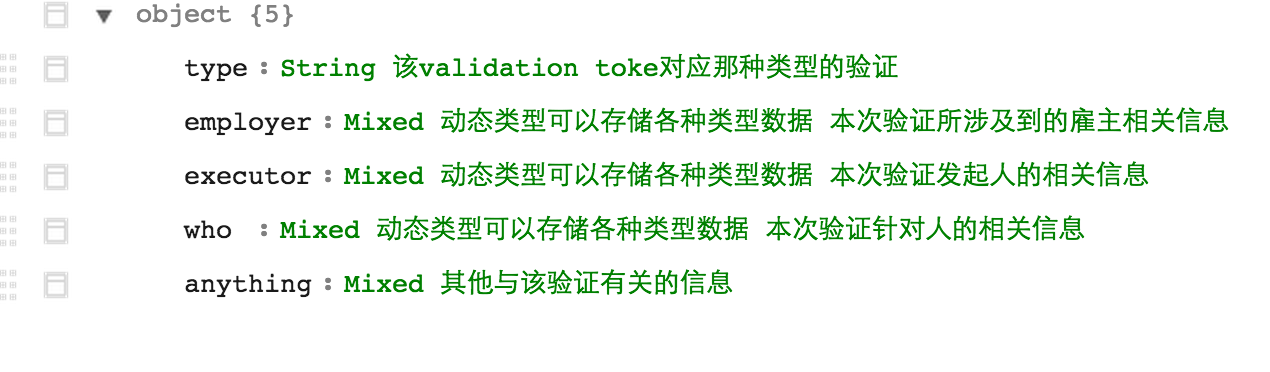
\includegraphics[width=0.8\textwidth]{validation.png}
	\figcaption{验证Token模型具体定义}
	\label{fig:validation-defined}
\end{figure}


\section{服务器端功能实现}

下面给出系统关键模块暴露出的api,和一些api的实现解释和细节

\subsection{Top Level 最上层代码}

下面给出整个app最顶层程序的伪代码


\hspace{1cm}
\begin{minipage}{1.0\linewidth}

\begin{Code}[label=index.js]
var config = require(app.config)
server = http.createServer(config.port);
socket_server = socket.io(server);
var modules  =  config.server_modules;

modules.forEach(function(module_name){
	var md = require(module_name);

	md.socket.forEach(function(obj){
		socket_server.on(obj.name, obj.function)
	});

	md.server.forEach(function(obj){
		server.inject(obj.method, obj.path, obj.function);
	});
});

server.listen(function(err){
	if(!err)
		console.log(server  started successfully.);
});
\end{Code}
\end{minipage}
\hspace{1cm}

其功能是

\begin{itemize}
\item 加载app的配置模块config
\item 根据app配置的端口创建Http服务器, 并由Http服务器创建Websocket服务器
\item 加载config中设置的要向服务器中导入的模块列表
\item 将所有加载的模块注入服务器
\item 开启服务器, app正式开始运行

\end{itemize}




\subsection{app.config模块}

里面要配置的内容为

\begin{itemize}
\item 服务器要运行哪个端口
\item 要加载的模块
\item 日志的粒度
\item 是否运行在DEBUG模式
\item 数据库的细节配置, 比如如何处理索引

\end{itemize}



\subsection{app.model模块和app.thunkify模块}

数据持久化层的定义, 前面已经说得很清楚了。

\subsection{app.log模块}

是app的日志模块, 对于一个web app来说, 日志记录非常重要。 日志记录有以下作用:

\begin{enumerate}
\item  检测黑客对于服务器攻击
\item 记录用户对于app的错误使用, 方便下一版本修改
\item 记录用户使用app的习惯, 用于更好的设计产品
\item 记录服务器出的错误,找出bug
\end{enumerate}



在该app中, 我记录日志的方法为:

\begin{quote}
  先写在一个文件中, 之后用一个定时运行的程序, 把该文件所有内容写入数据库。作为数据的持久化。
\end{quote}


记录日志的种类为:

\begin{itemize}
\item DEBUG 调试信息
\item TRACE 也是只有调试的时候会用,细节信息, 比如进入了哪个函数等等
\item ERROR 发生的系统错误
\item WARN  系统的警告, 比如疑似的攻击
\item INFO  用户操作的记录
\end{itemize}





\subsection{app.privilege模块}

该模块管理系统提供了管理教师用户的权限机制

分为:
\begin{itemize}
\item HumanResource 可以管理班级内的人员
\item InfoManager 可以在任何班级和自己雇主的学校发布通知, 和修改班级, 学校介绍
\item BOSS 拥有所有权限(不只是上面的两种操作, 比如学校名称的修改)
\end{itemize}

通过或操作来完成权限的相加, 与非操作来完成权限的相减。



\subsection{app.notice模块}

使用了sendcloud.sohu.com和极光推送的服务, 完成发短信,发邮件通知和手机端Push Notification的功能。

需要通知的操作一般为:

\begin{itemize}
\item 人员的转班, 邀请等等
\item 手机端聊天的提醒
\item 忘记密码
\end{itemize}




\subsection{app.data命名空间}

在空间下, 是对于底层数据定义的抽象层

\subsubsection{class班级和school学校}

\begin{itemize}
\item 提供学校班级的创建,修改,删除
\item 这里删除使用软删除,不真正删除数据而是用一个Deleted的布尔标记
\item 人员转班转校
\end{itemize}

\subsubsection{post状态}

\begin{itemize}
\item 发送状态
\item 删除所发状态
\end{itemize}

\subsubsection{file文件和image图片}

\begin{itemize}
\item 文件的删除,修改, 新建
\item 文件夹的展开
\item 删除依旧使用软删除
\item 相册是一个只有一层的文件夹
\end{itemize}



\subsubsection{app.validationToken模块}

处理申请request操作


\begin{itemize}
\item 比如用户提交转班,邀请某人加入某班的申请, 该模块会创建一个validationToken

\item validationToken创建的时候, 会执行验证的Pre函数, 该函数会根据该Token的类型, 来执行验证的预操作, 比如改变用户的状态。

\item 当用户点击验证连接同意验证的时候, 该模块会根据Token的类型, 执行Post函数, 完成验证的后续操作, 真正改变用户班级归属。
\end{itemize}





\section{Web管理端界面设计}

\begin{itemize}

\item 学校信息界面

\begin{figure}[H]
  \centering
  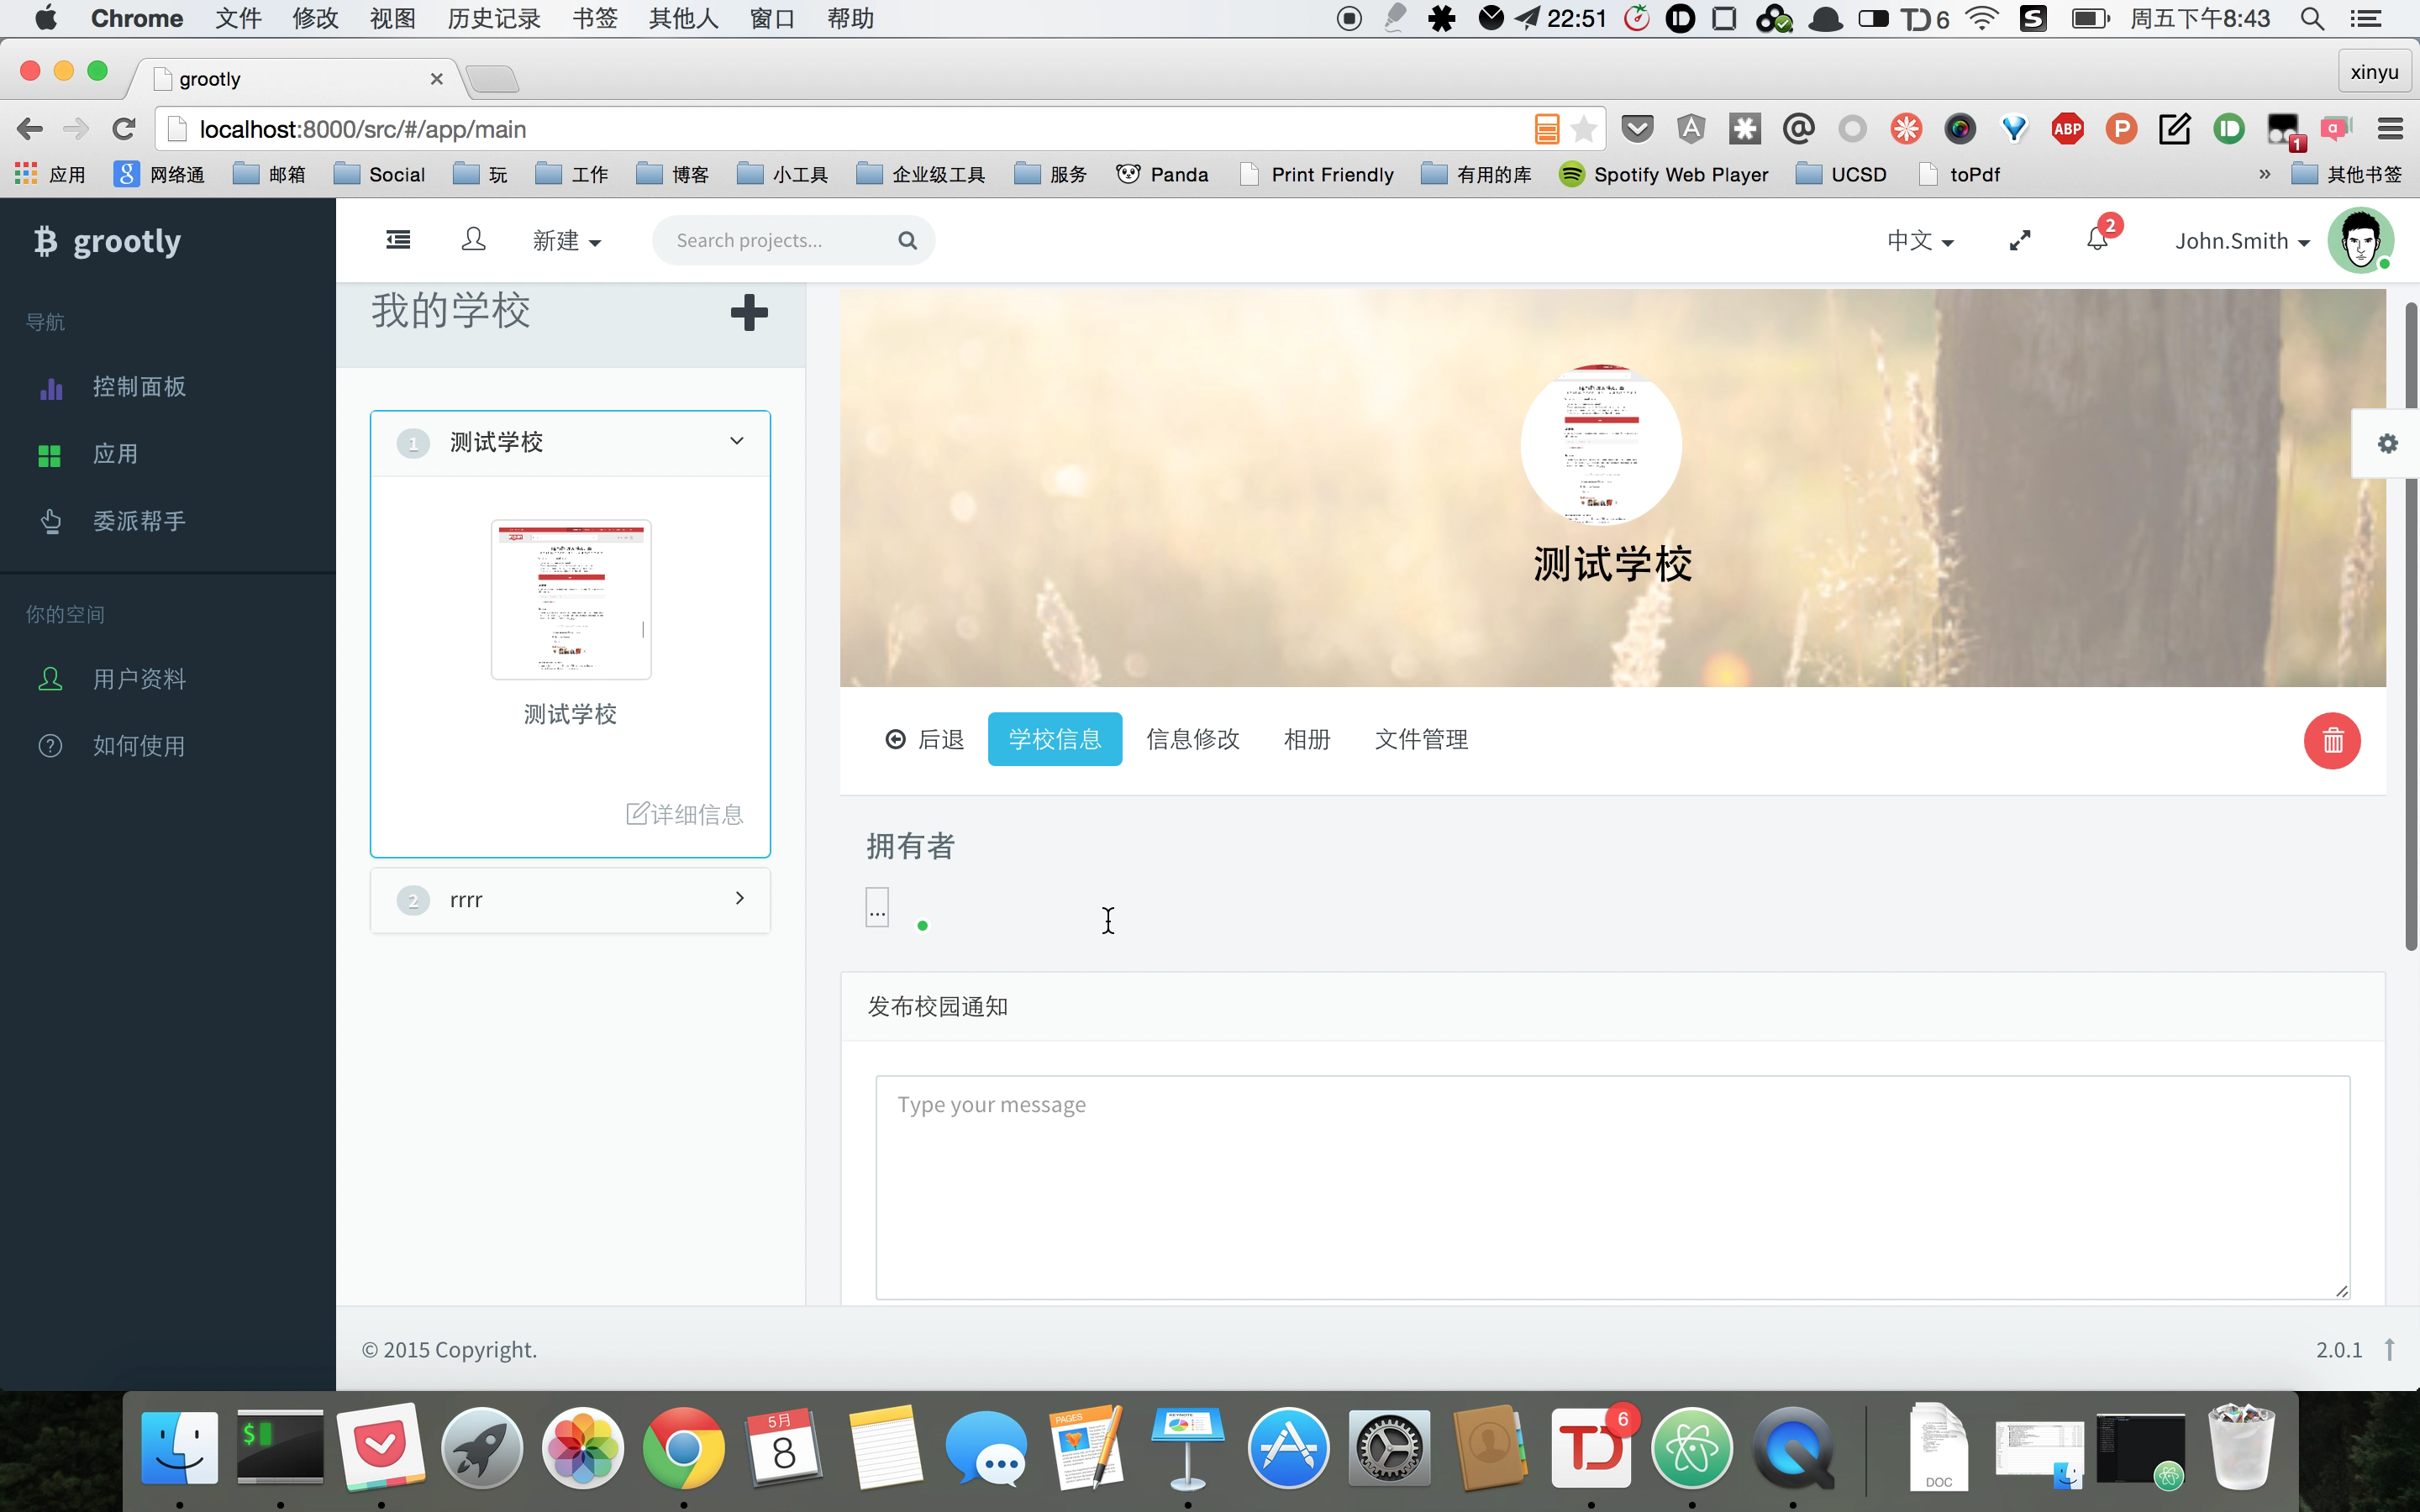
\includegraphics[width=0.7\textwidth]{school_page.png}
  \figcaption{Web管理端 学校信息界面}
  \label{fig: pc_schoolinfo}
\end{figure}


\item 班级列表界面

\begin{figure}[H]
  \centering
  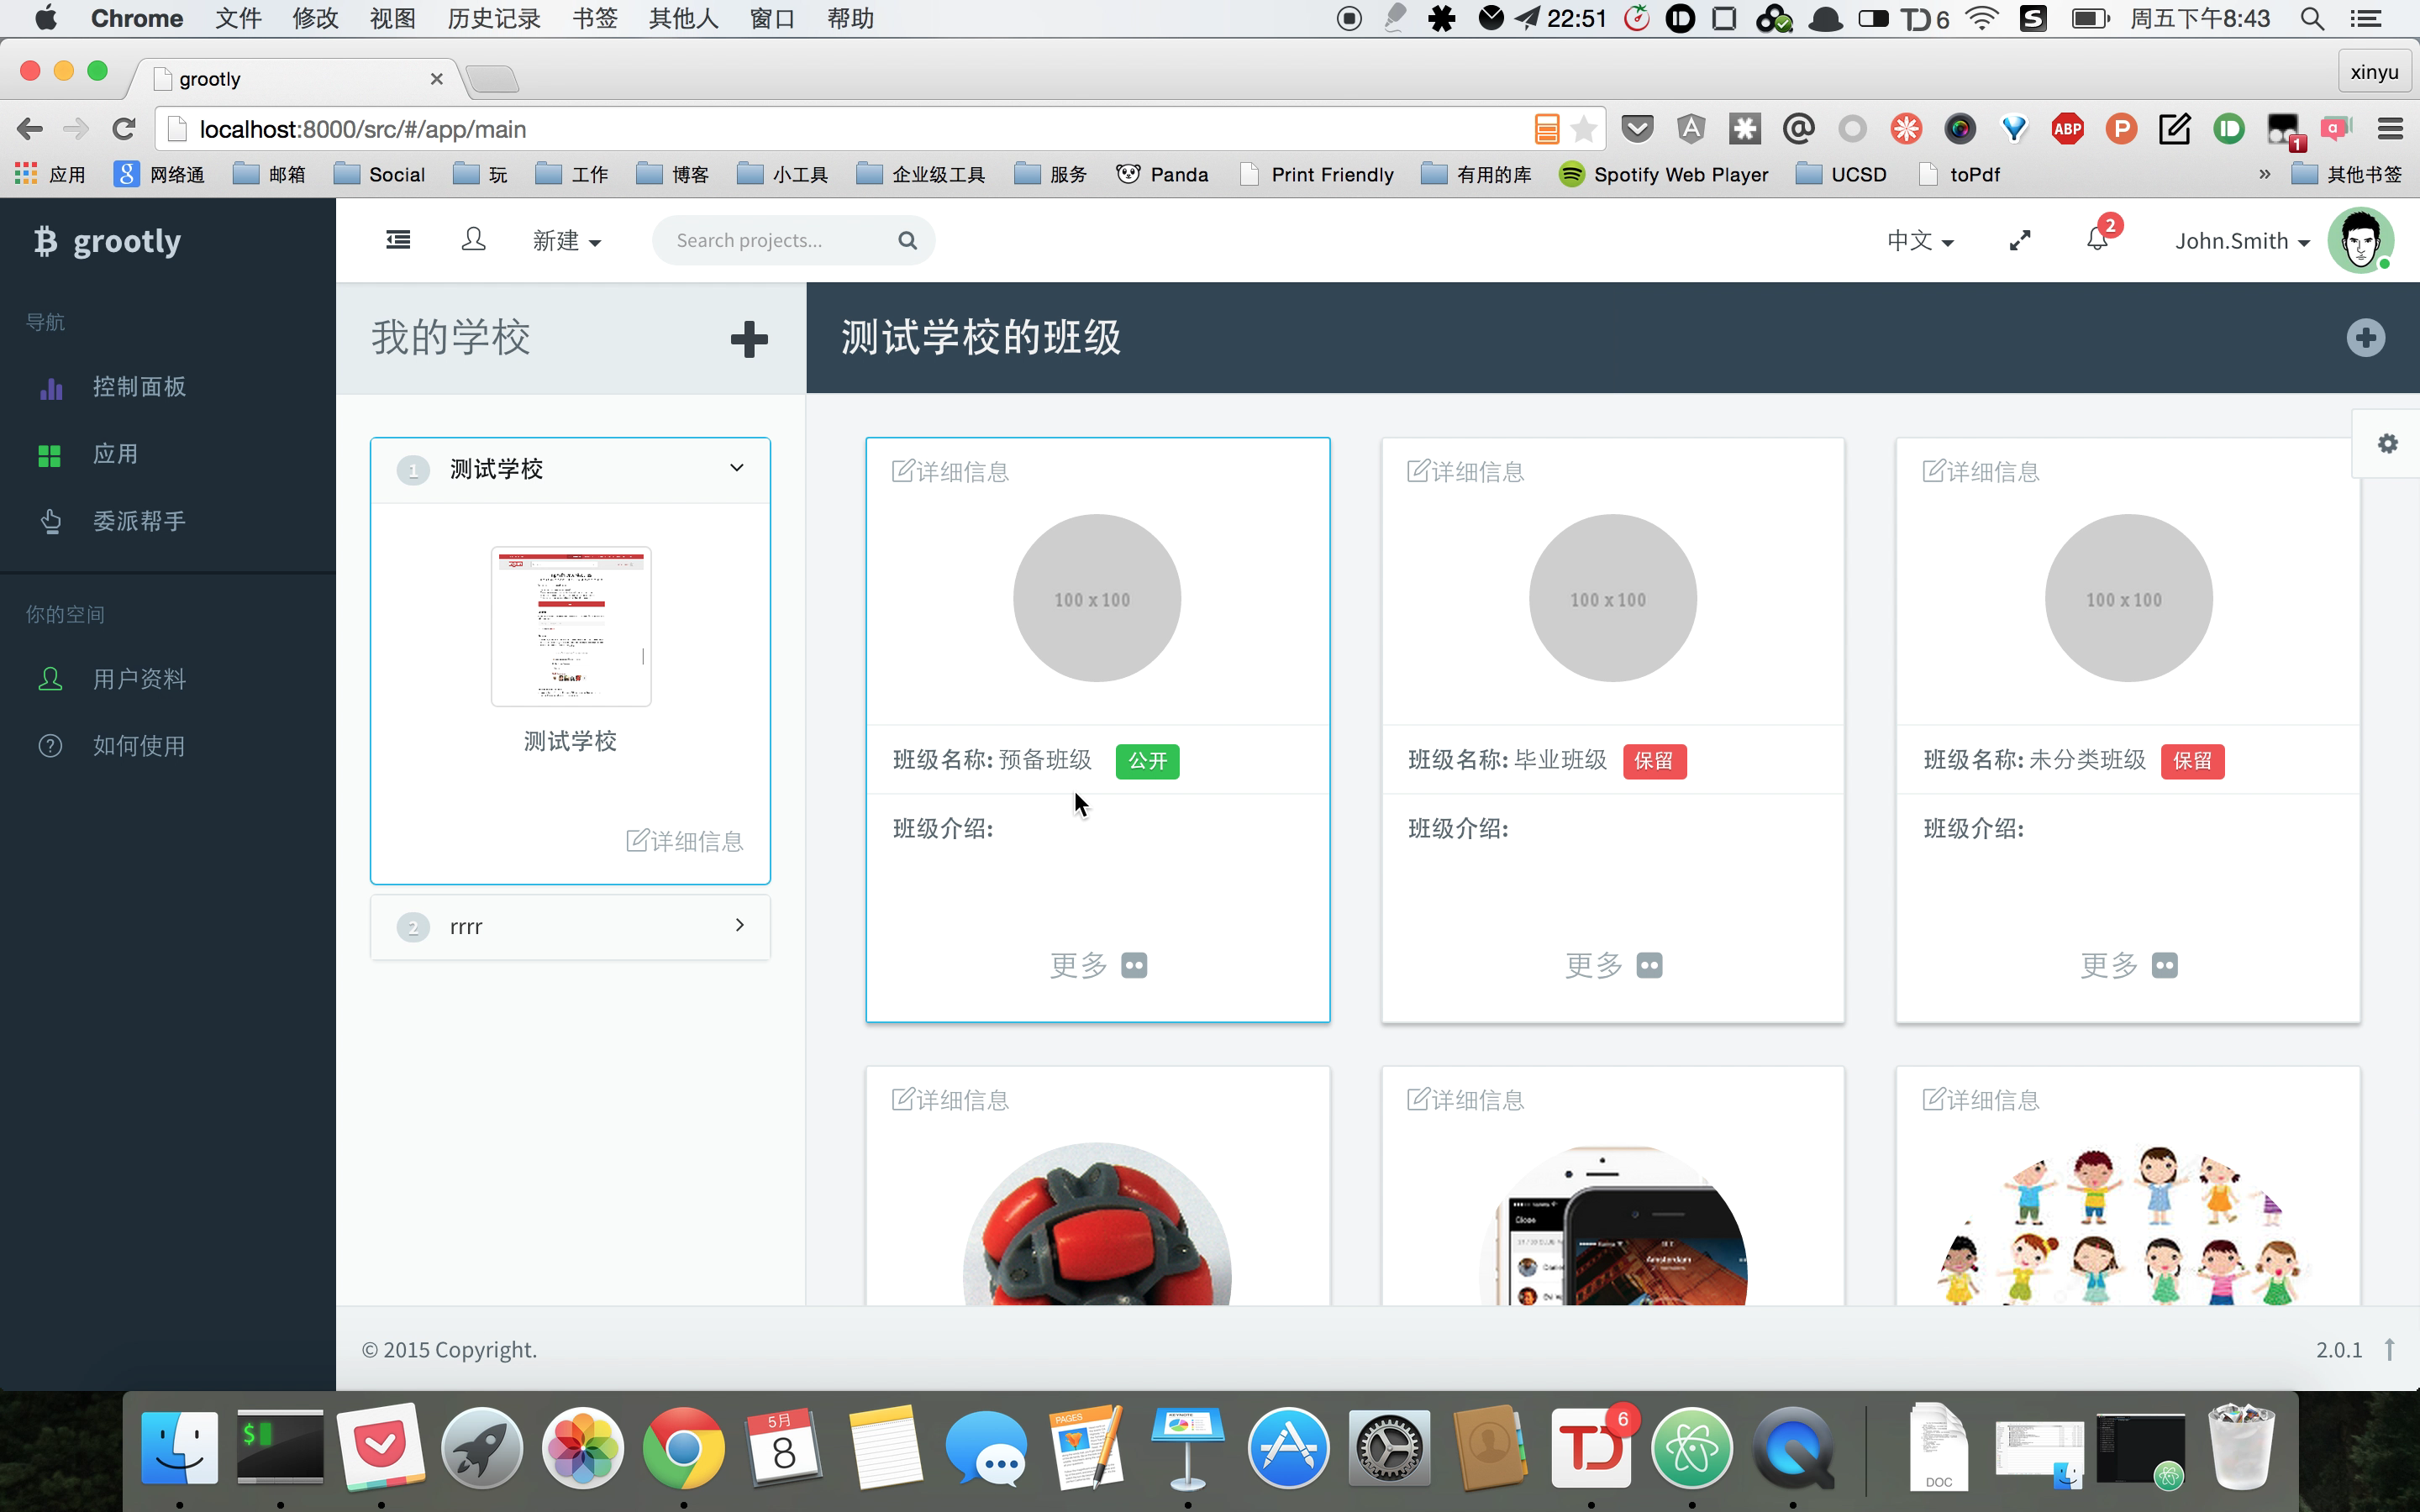
\includegraphics[width=0.7\textwidth]{my_class_list.png}
  \figcaption{Web管理端 班级列表界面}
  \label{fig: pc_classlist}
\end{figure}


\item 网盘界面

\begin{figure}[H]
  \centering
  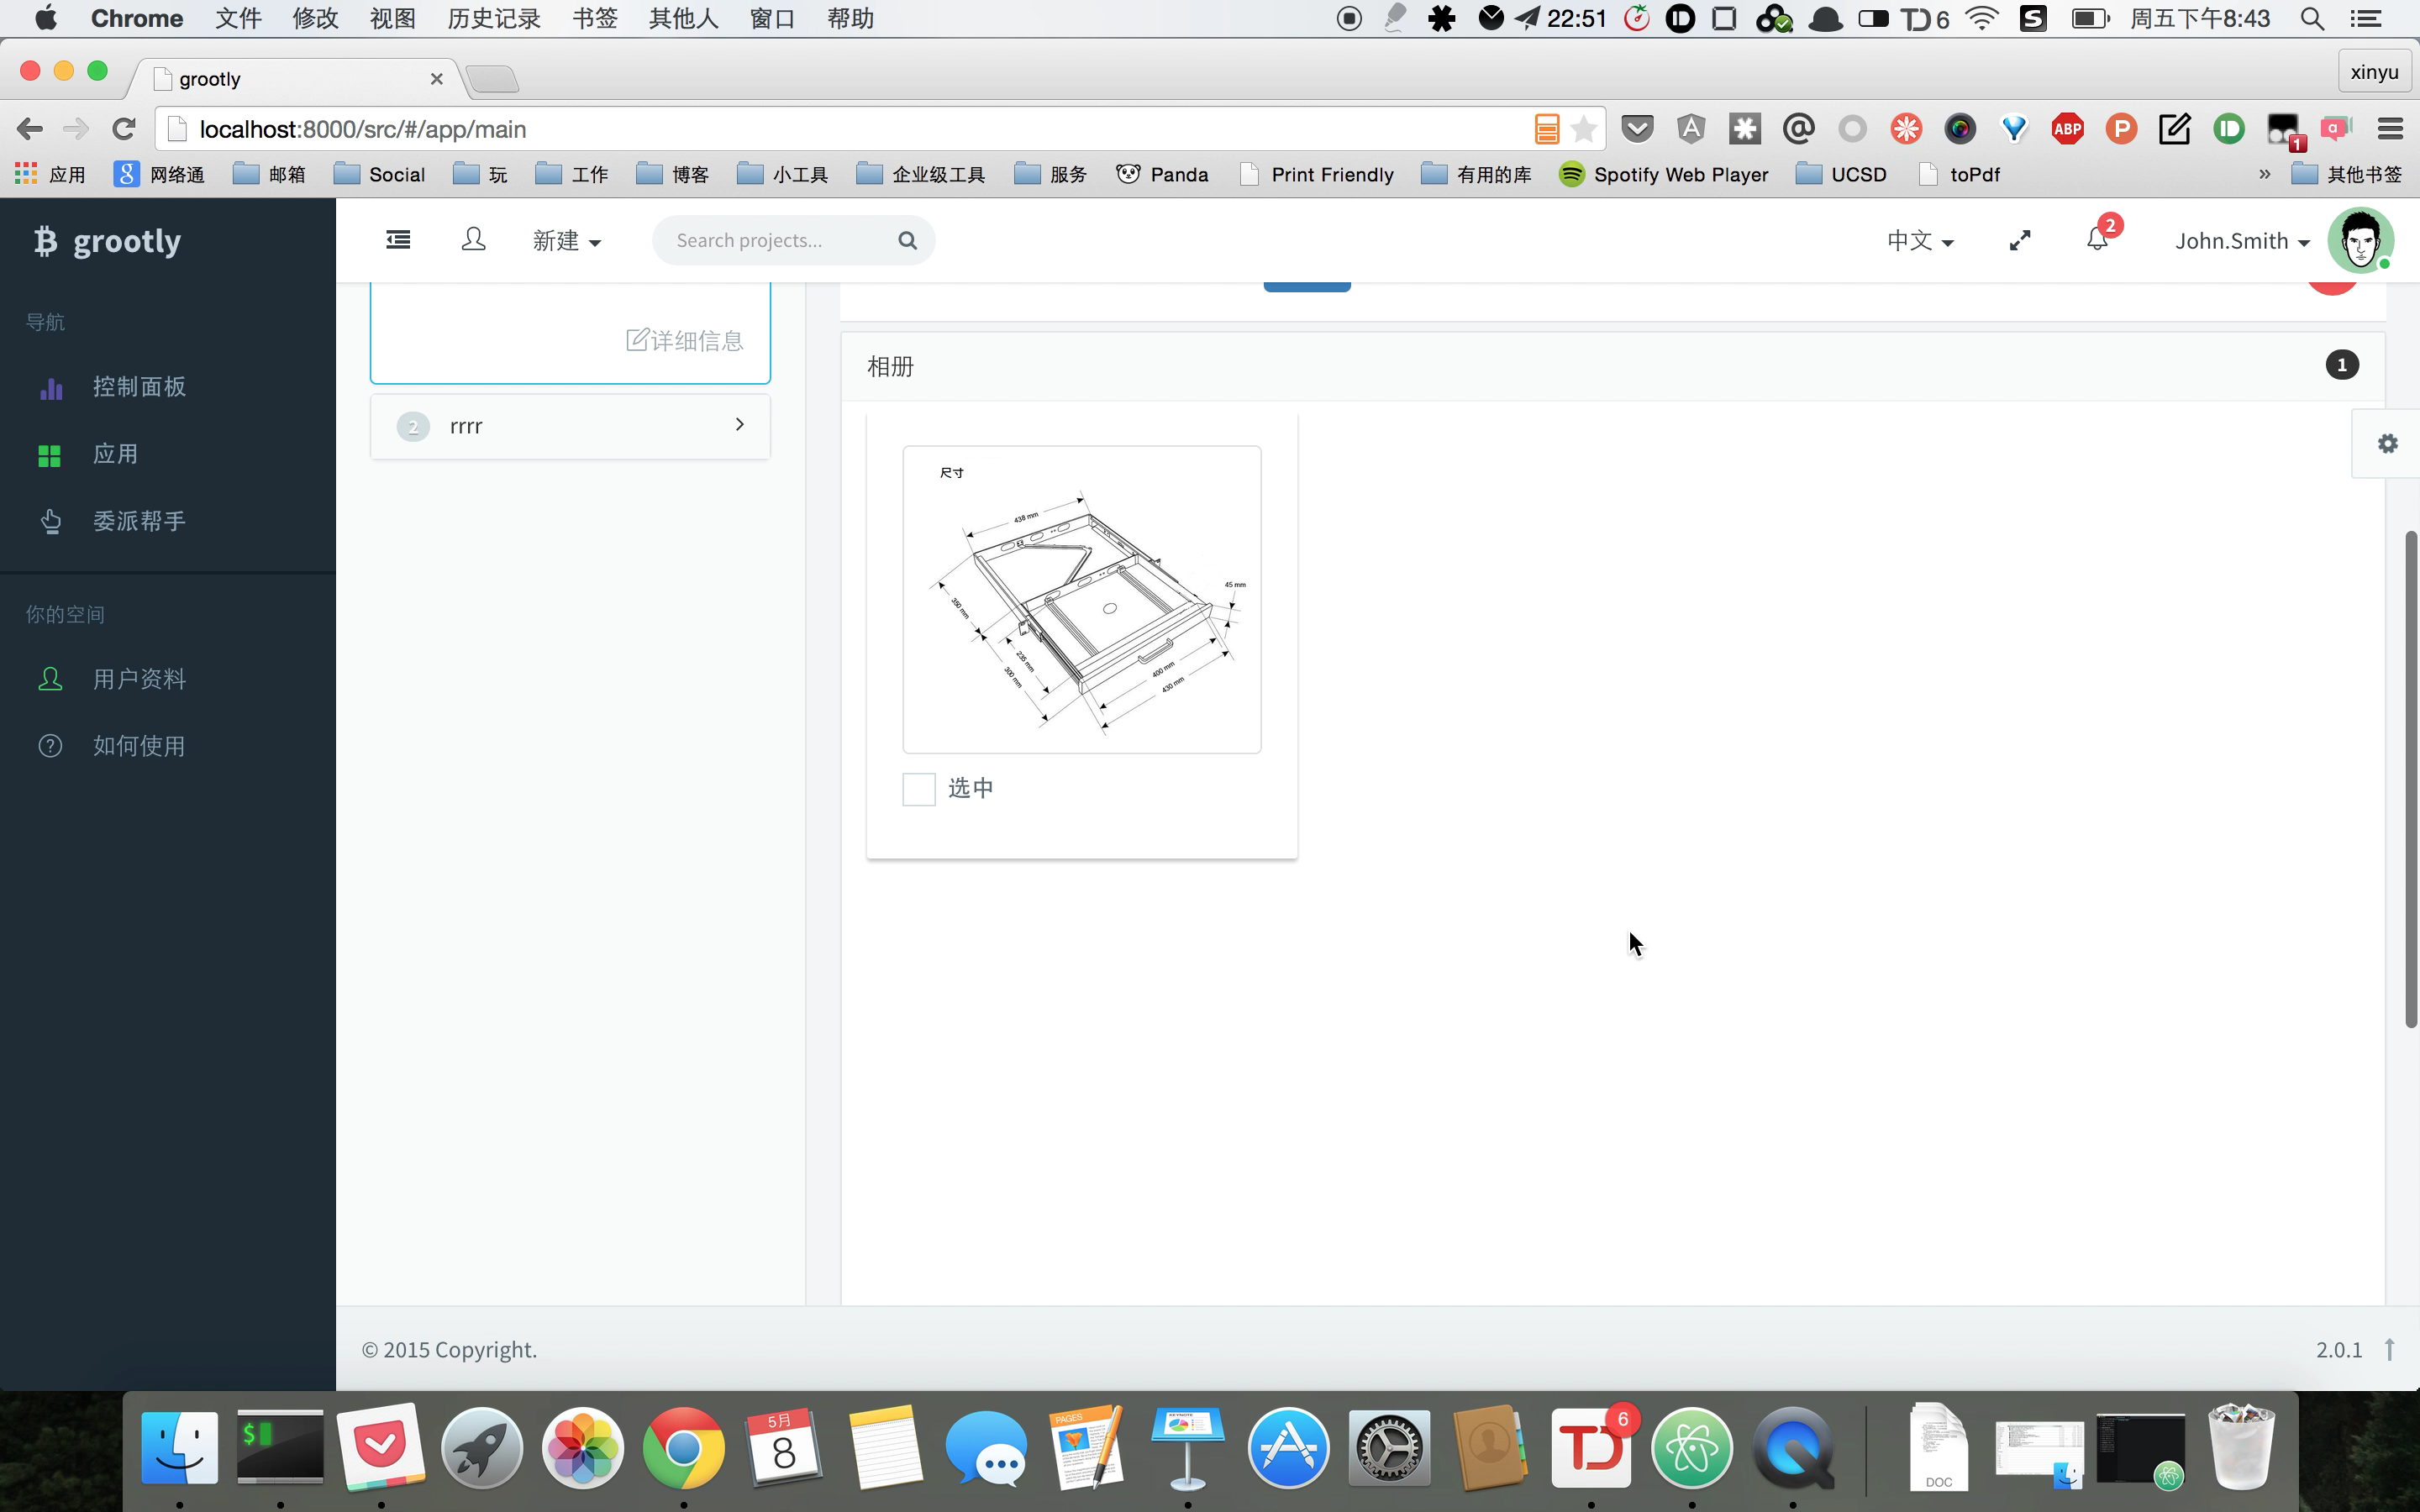
\includegraphics[width=0.7\textwidth]{album1.png}
  \figcaption{Web管理端 相册界面1}
  \label{fig: pc_album1}
\end{figure}



\begin{figure}[H]
  \centering
  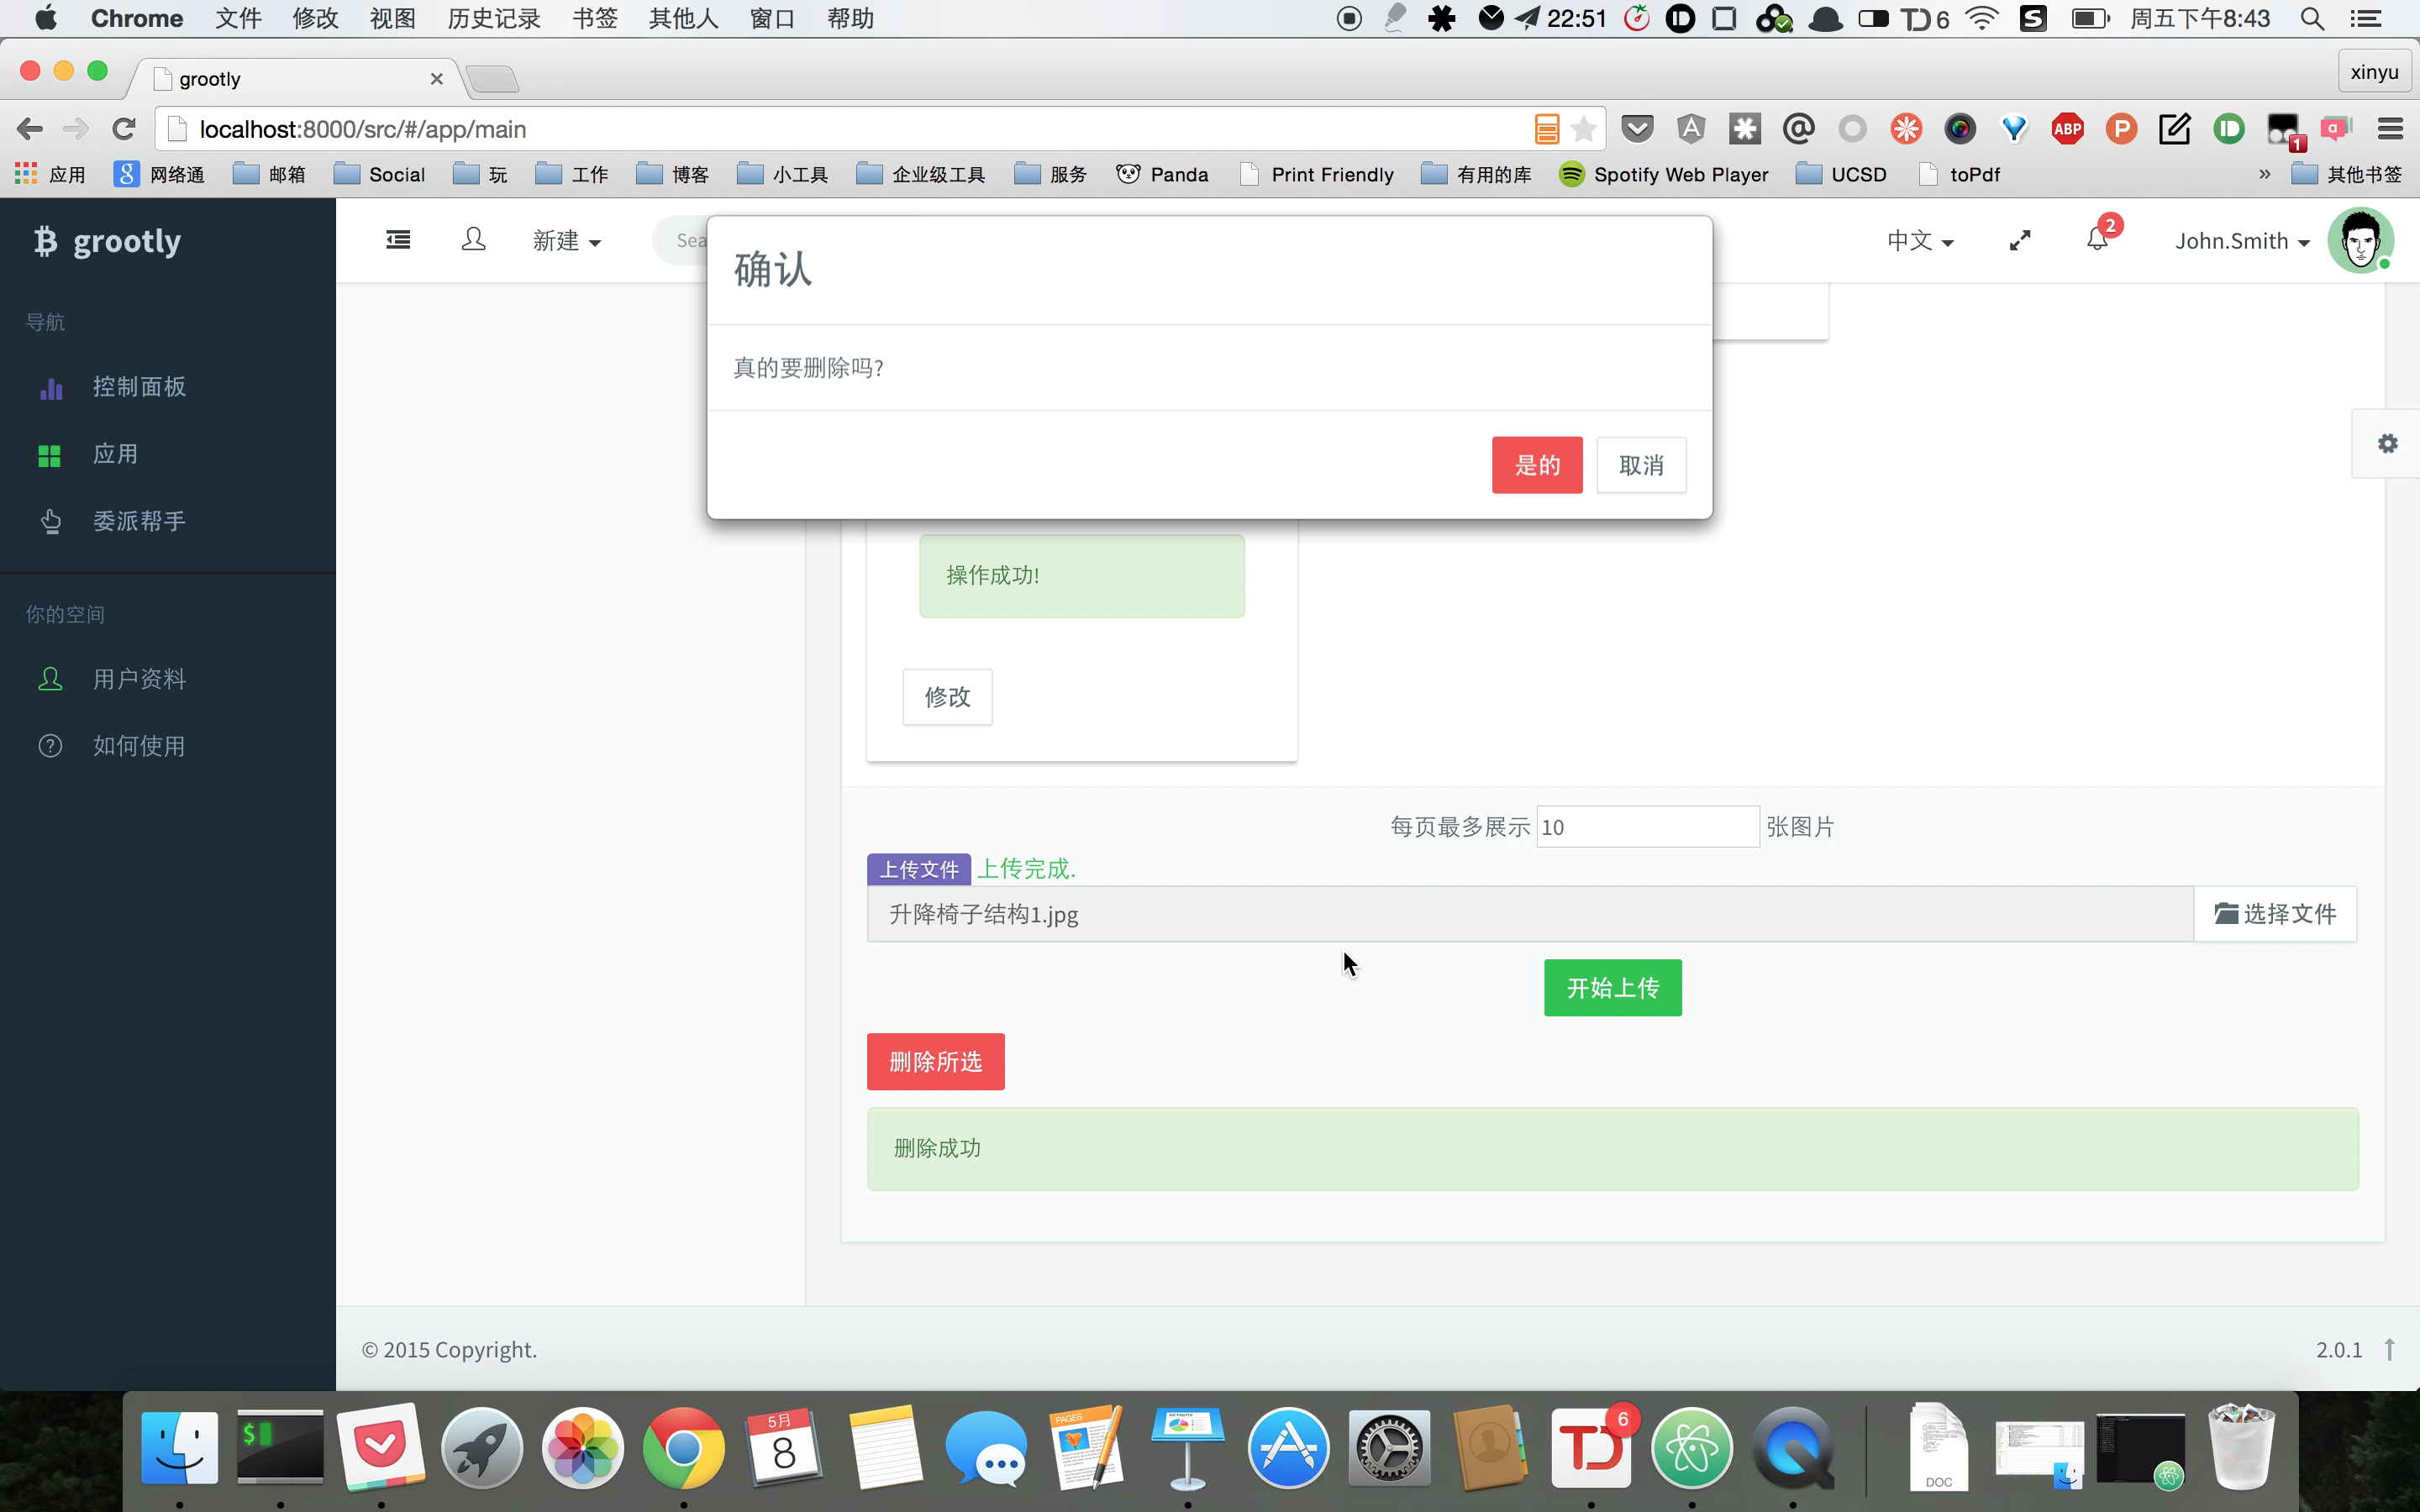
\includegraphics[width=0.7\textwidth]{album2.png}
  \figcaption{Web管理端 相册界面2}
  \label{fig: pc_album2}
\end{figure}


\item 相册界面

\begin{figure}[H]
  \centering
  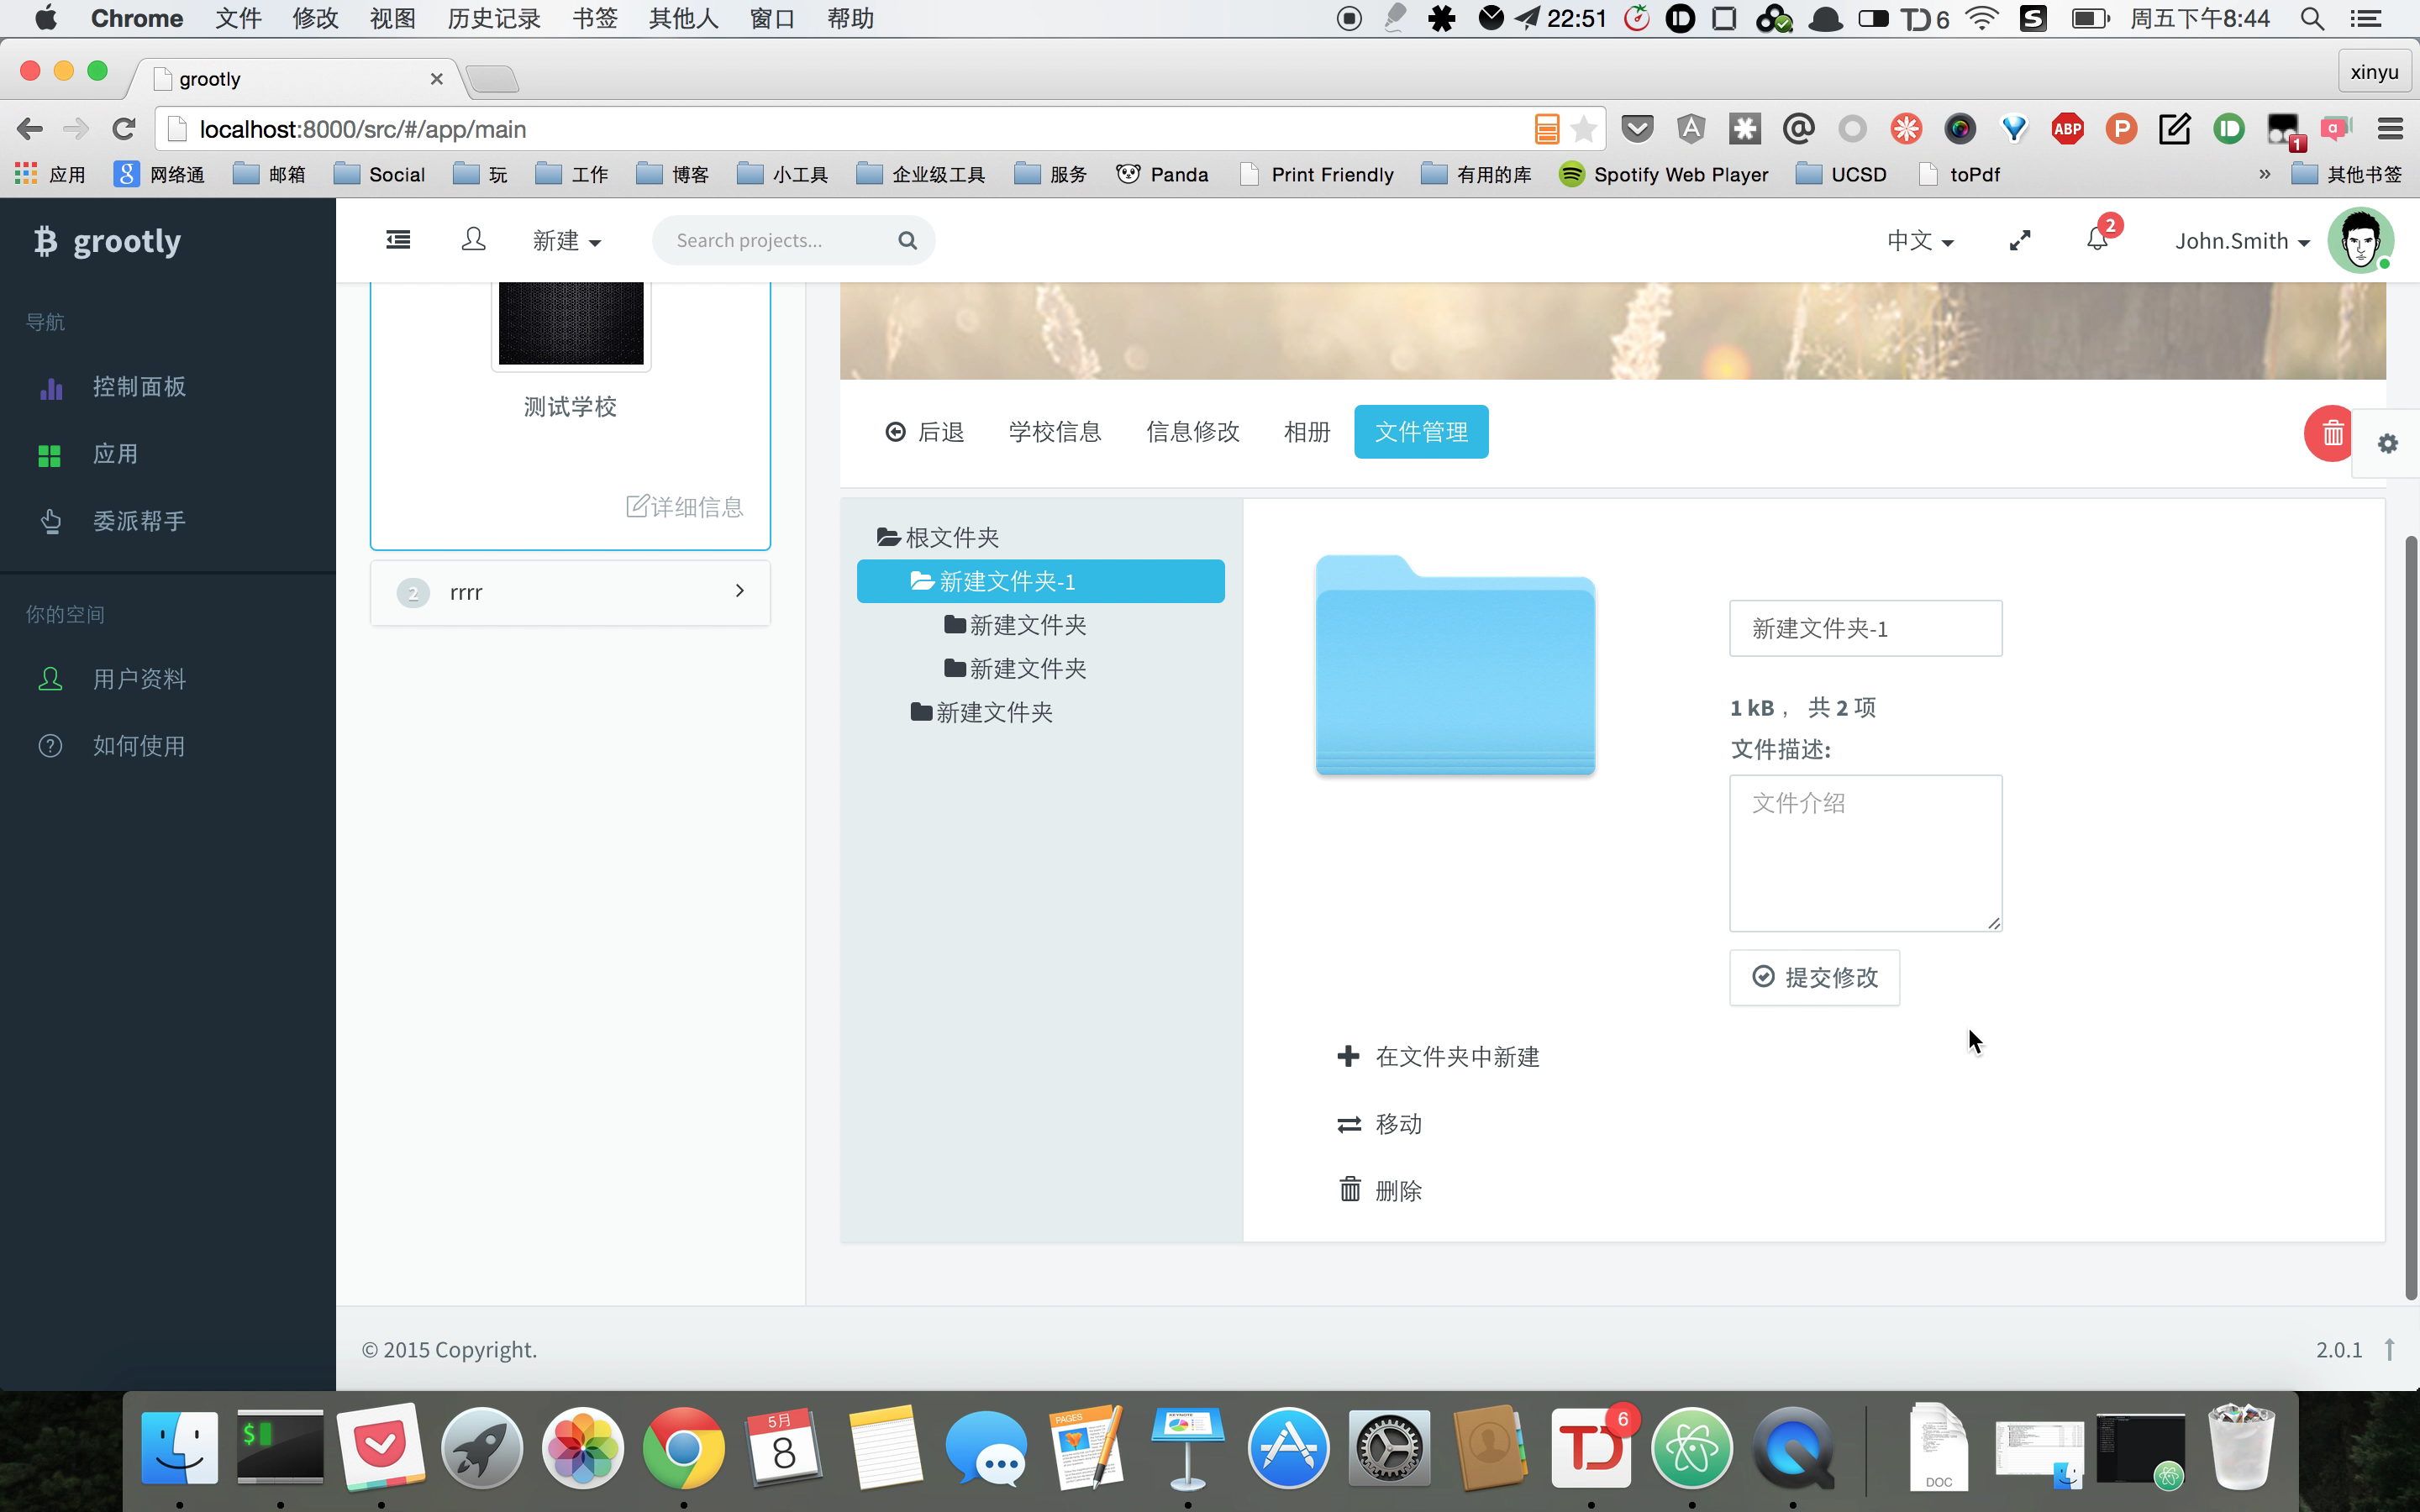
\includegraphics[width=0.7\textwidth]{pan1.png}
  \figcaption{Web管理端 网盘界面1}
  \label{fig: pc_pan1}
\end{figure}



\begin{figure}[H]
  \centering
  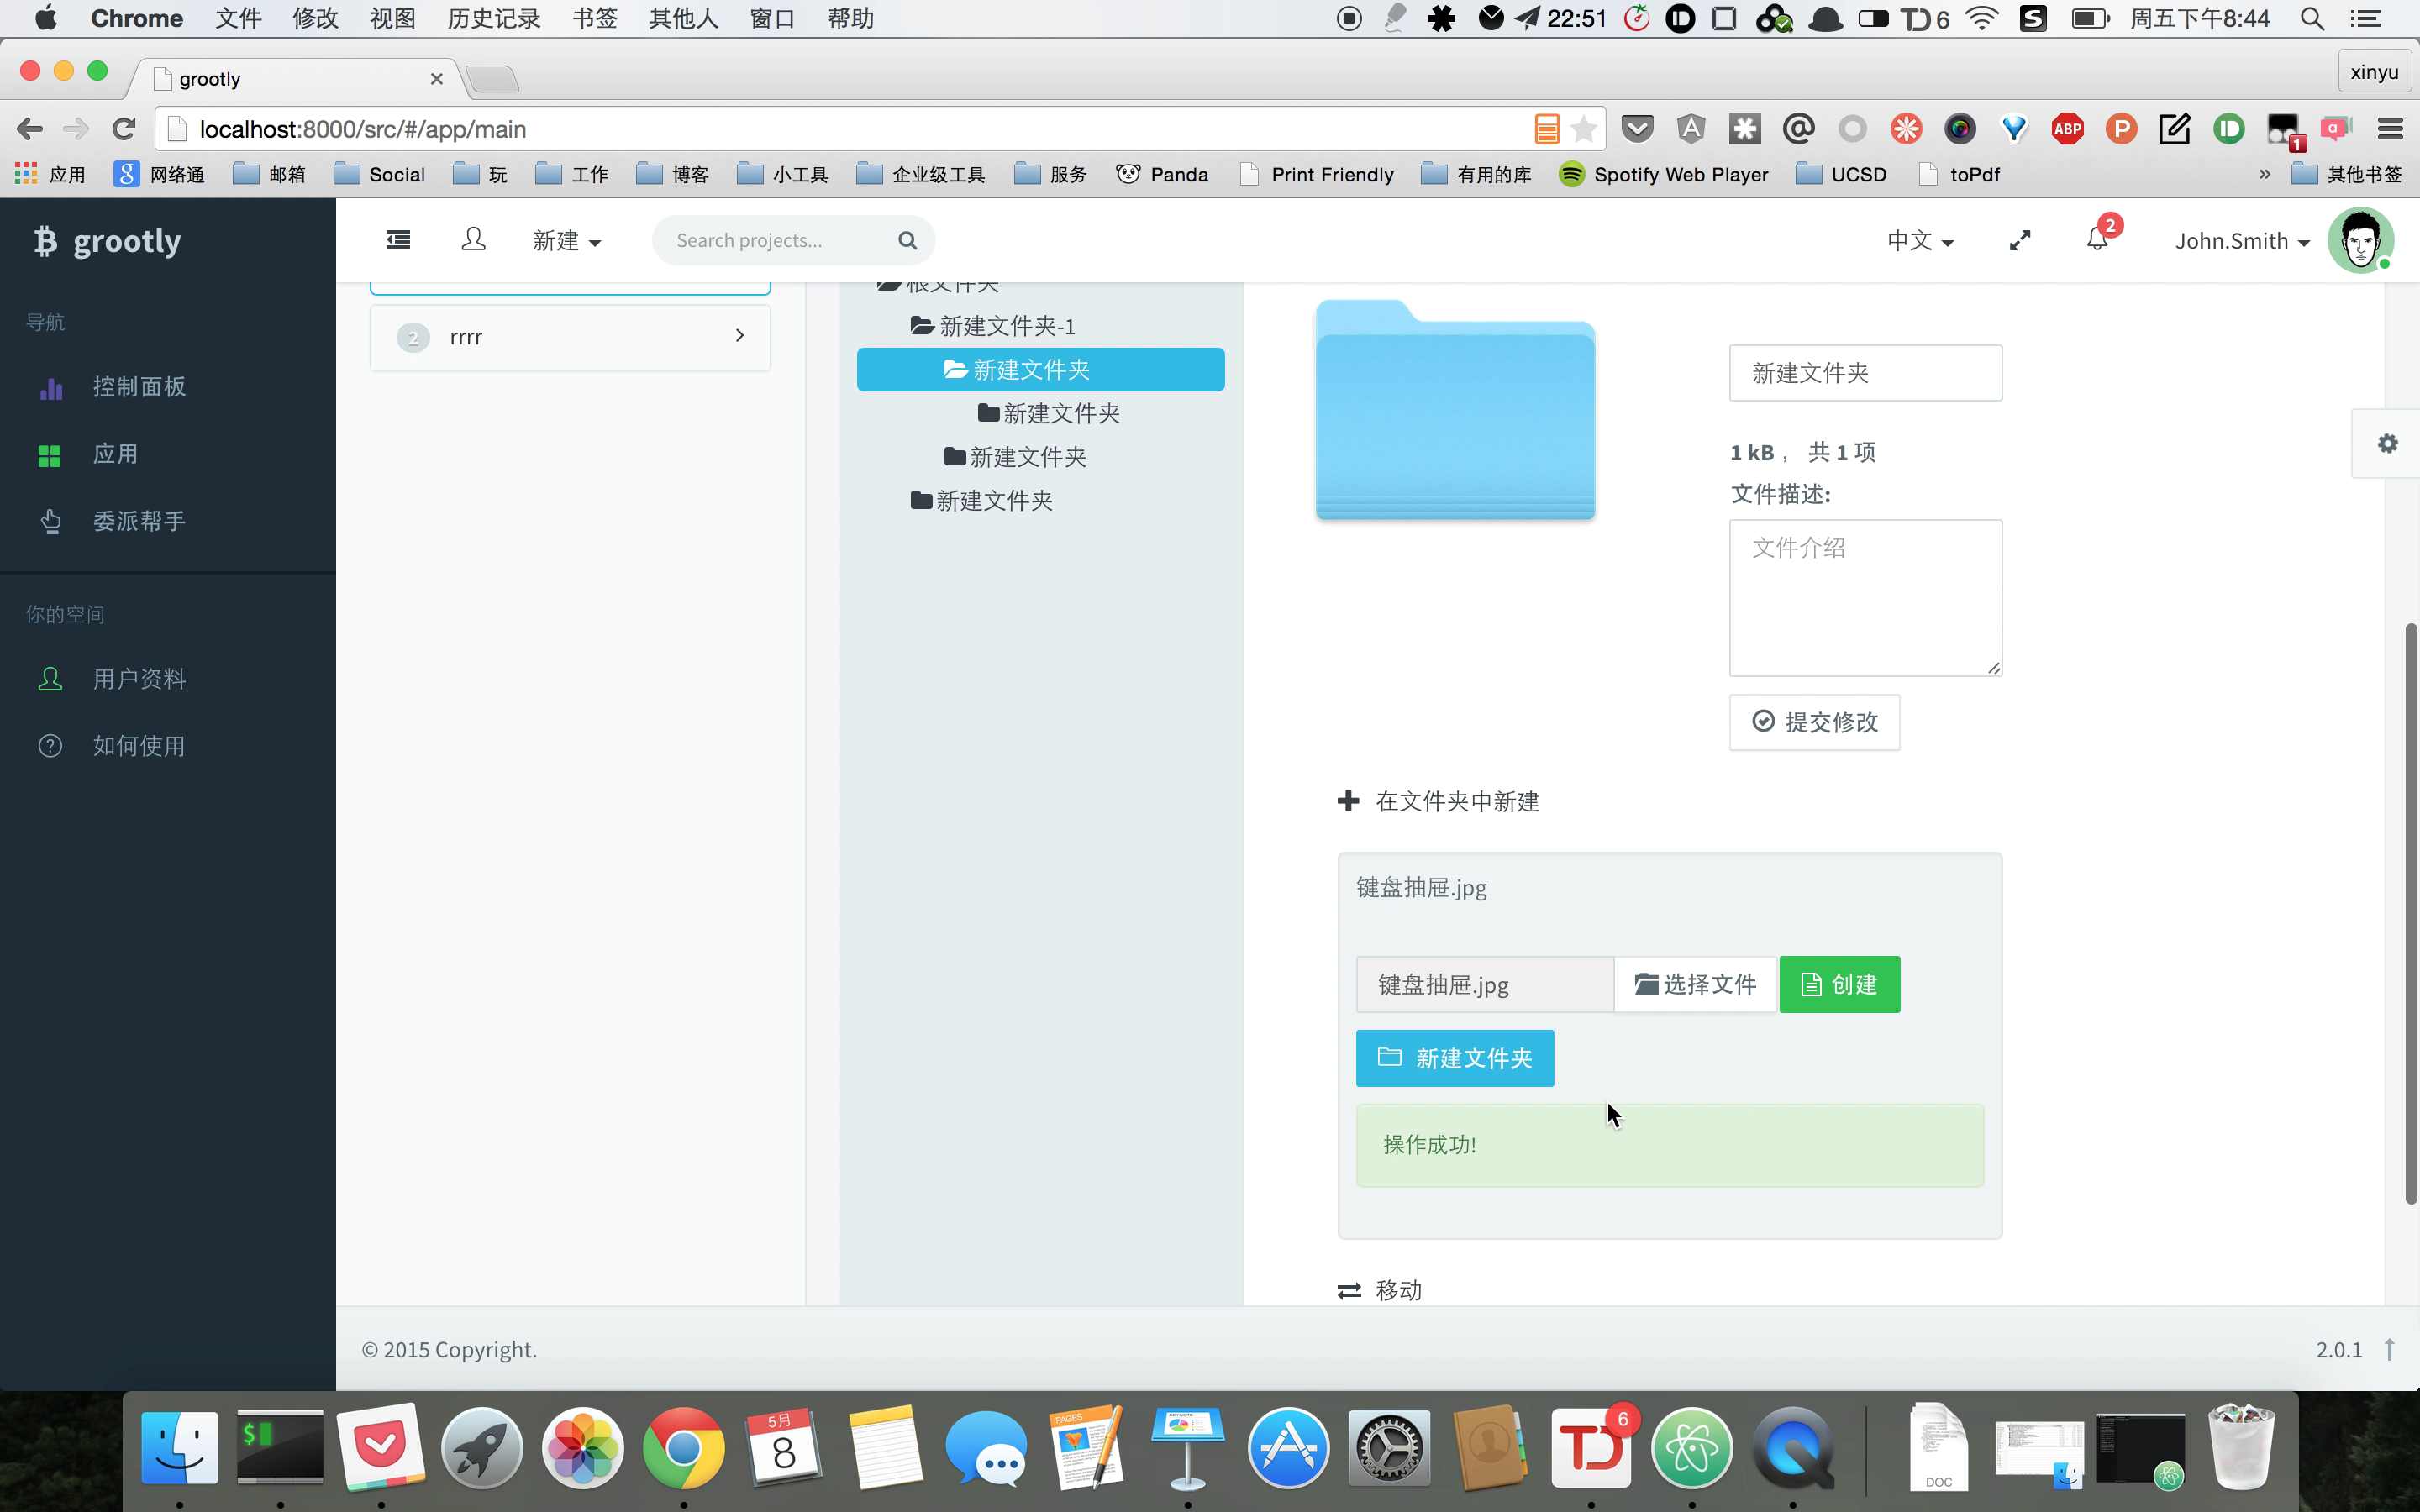
\includegraphics[width=0.7\textwidth]{pan2.png}
  \figcaption{Web管理端 网盘界面2}
  \label{fig: pc_pan2}
\end{figure}



\item 教师,学生的管理界面

\begin{figure}[H]
  \centering
  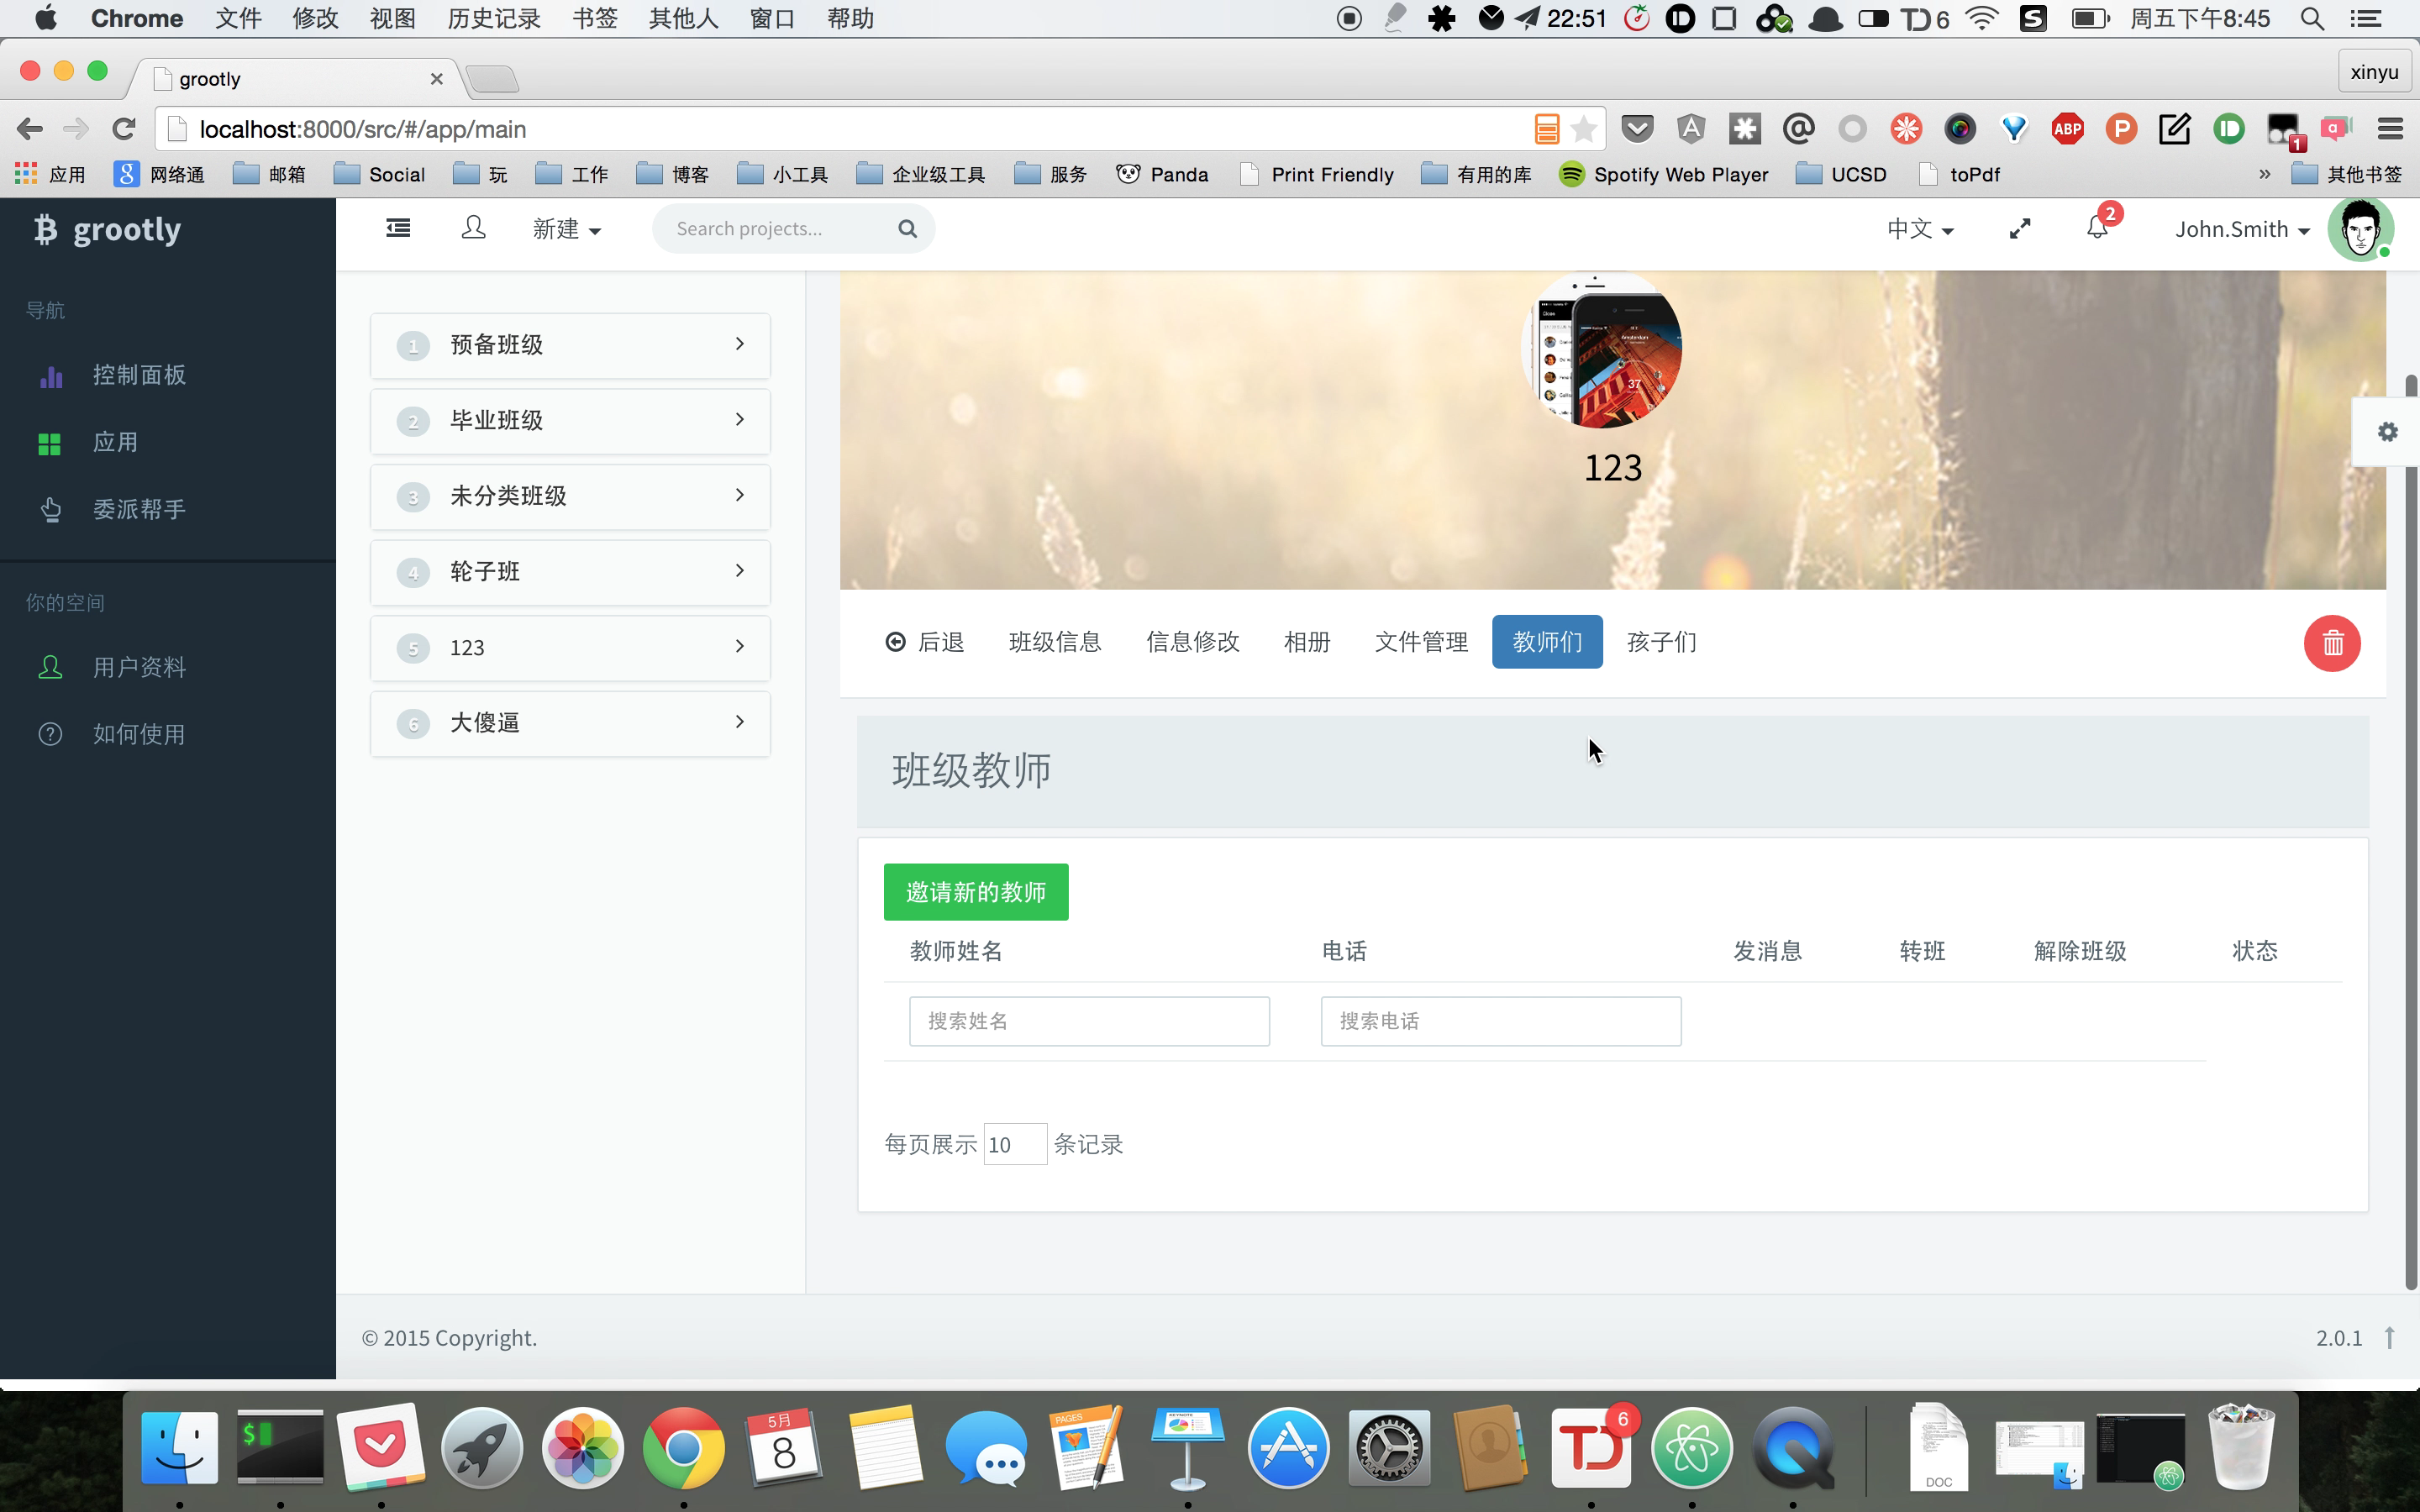
\includegraphics[width=0.7\textwidth]{my_teacher.png}
  \figcaption{Web管理端 教师列表界面}
  \label{fig: pc_my_teacher}
\end{figure}


\begin{figure}[H]
  \centering
  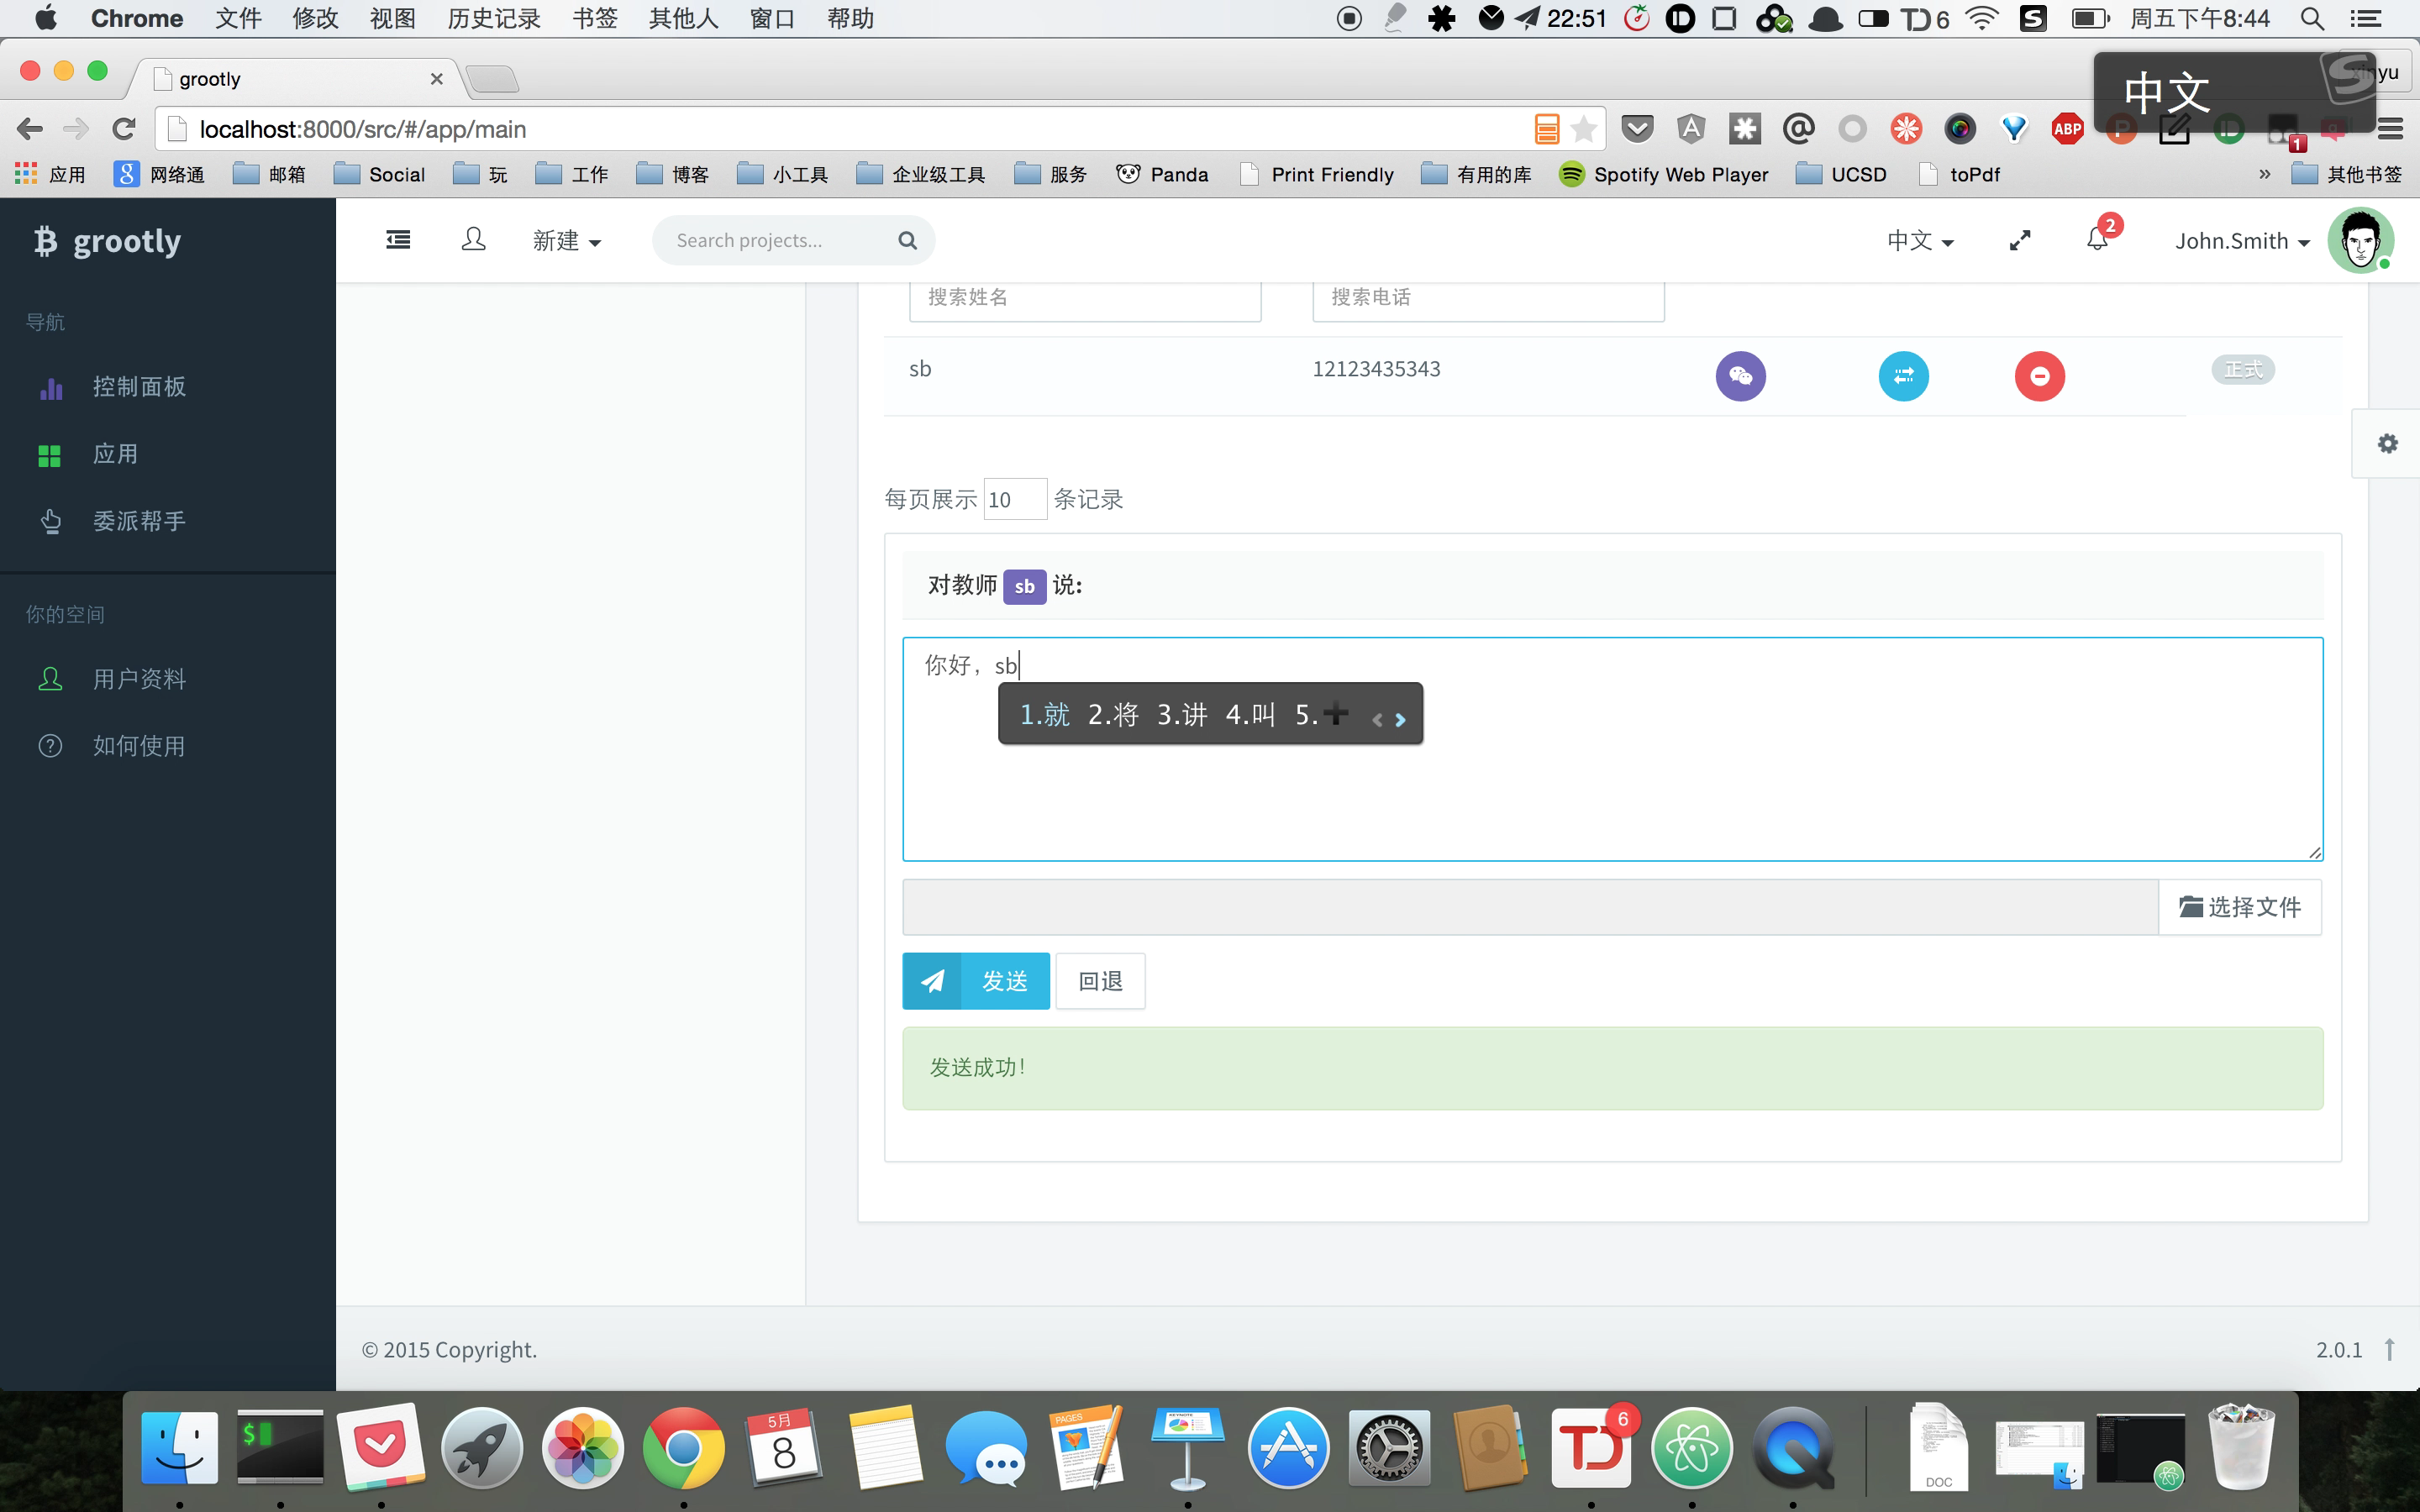
\includegraphics[width=0.7\textwidth]{people_post.png}
  \figcaption{Web管理端 人员发布通知界面}
  \label{fig: pc_people_post}
\end{figure}

\begin{figure}[H]
  \centering
  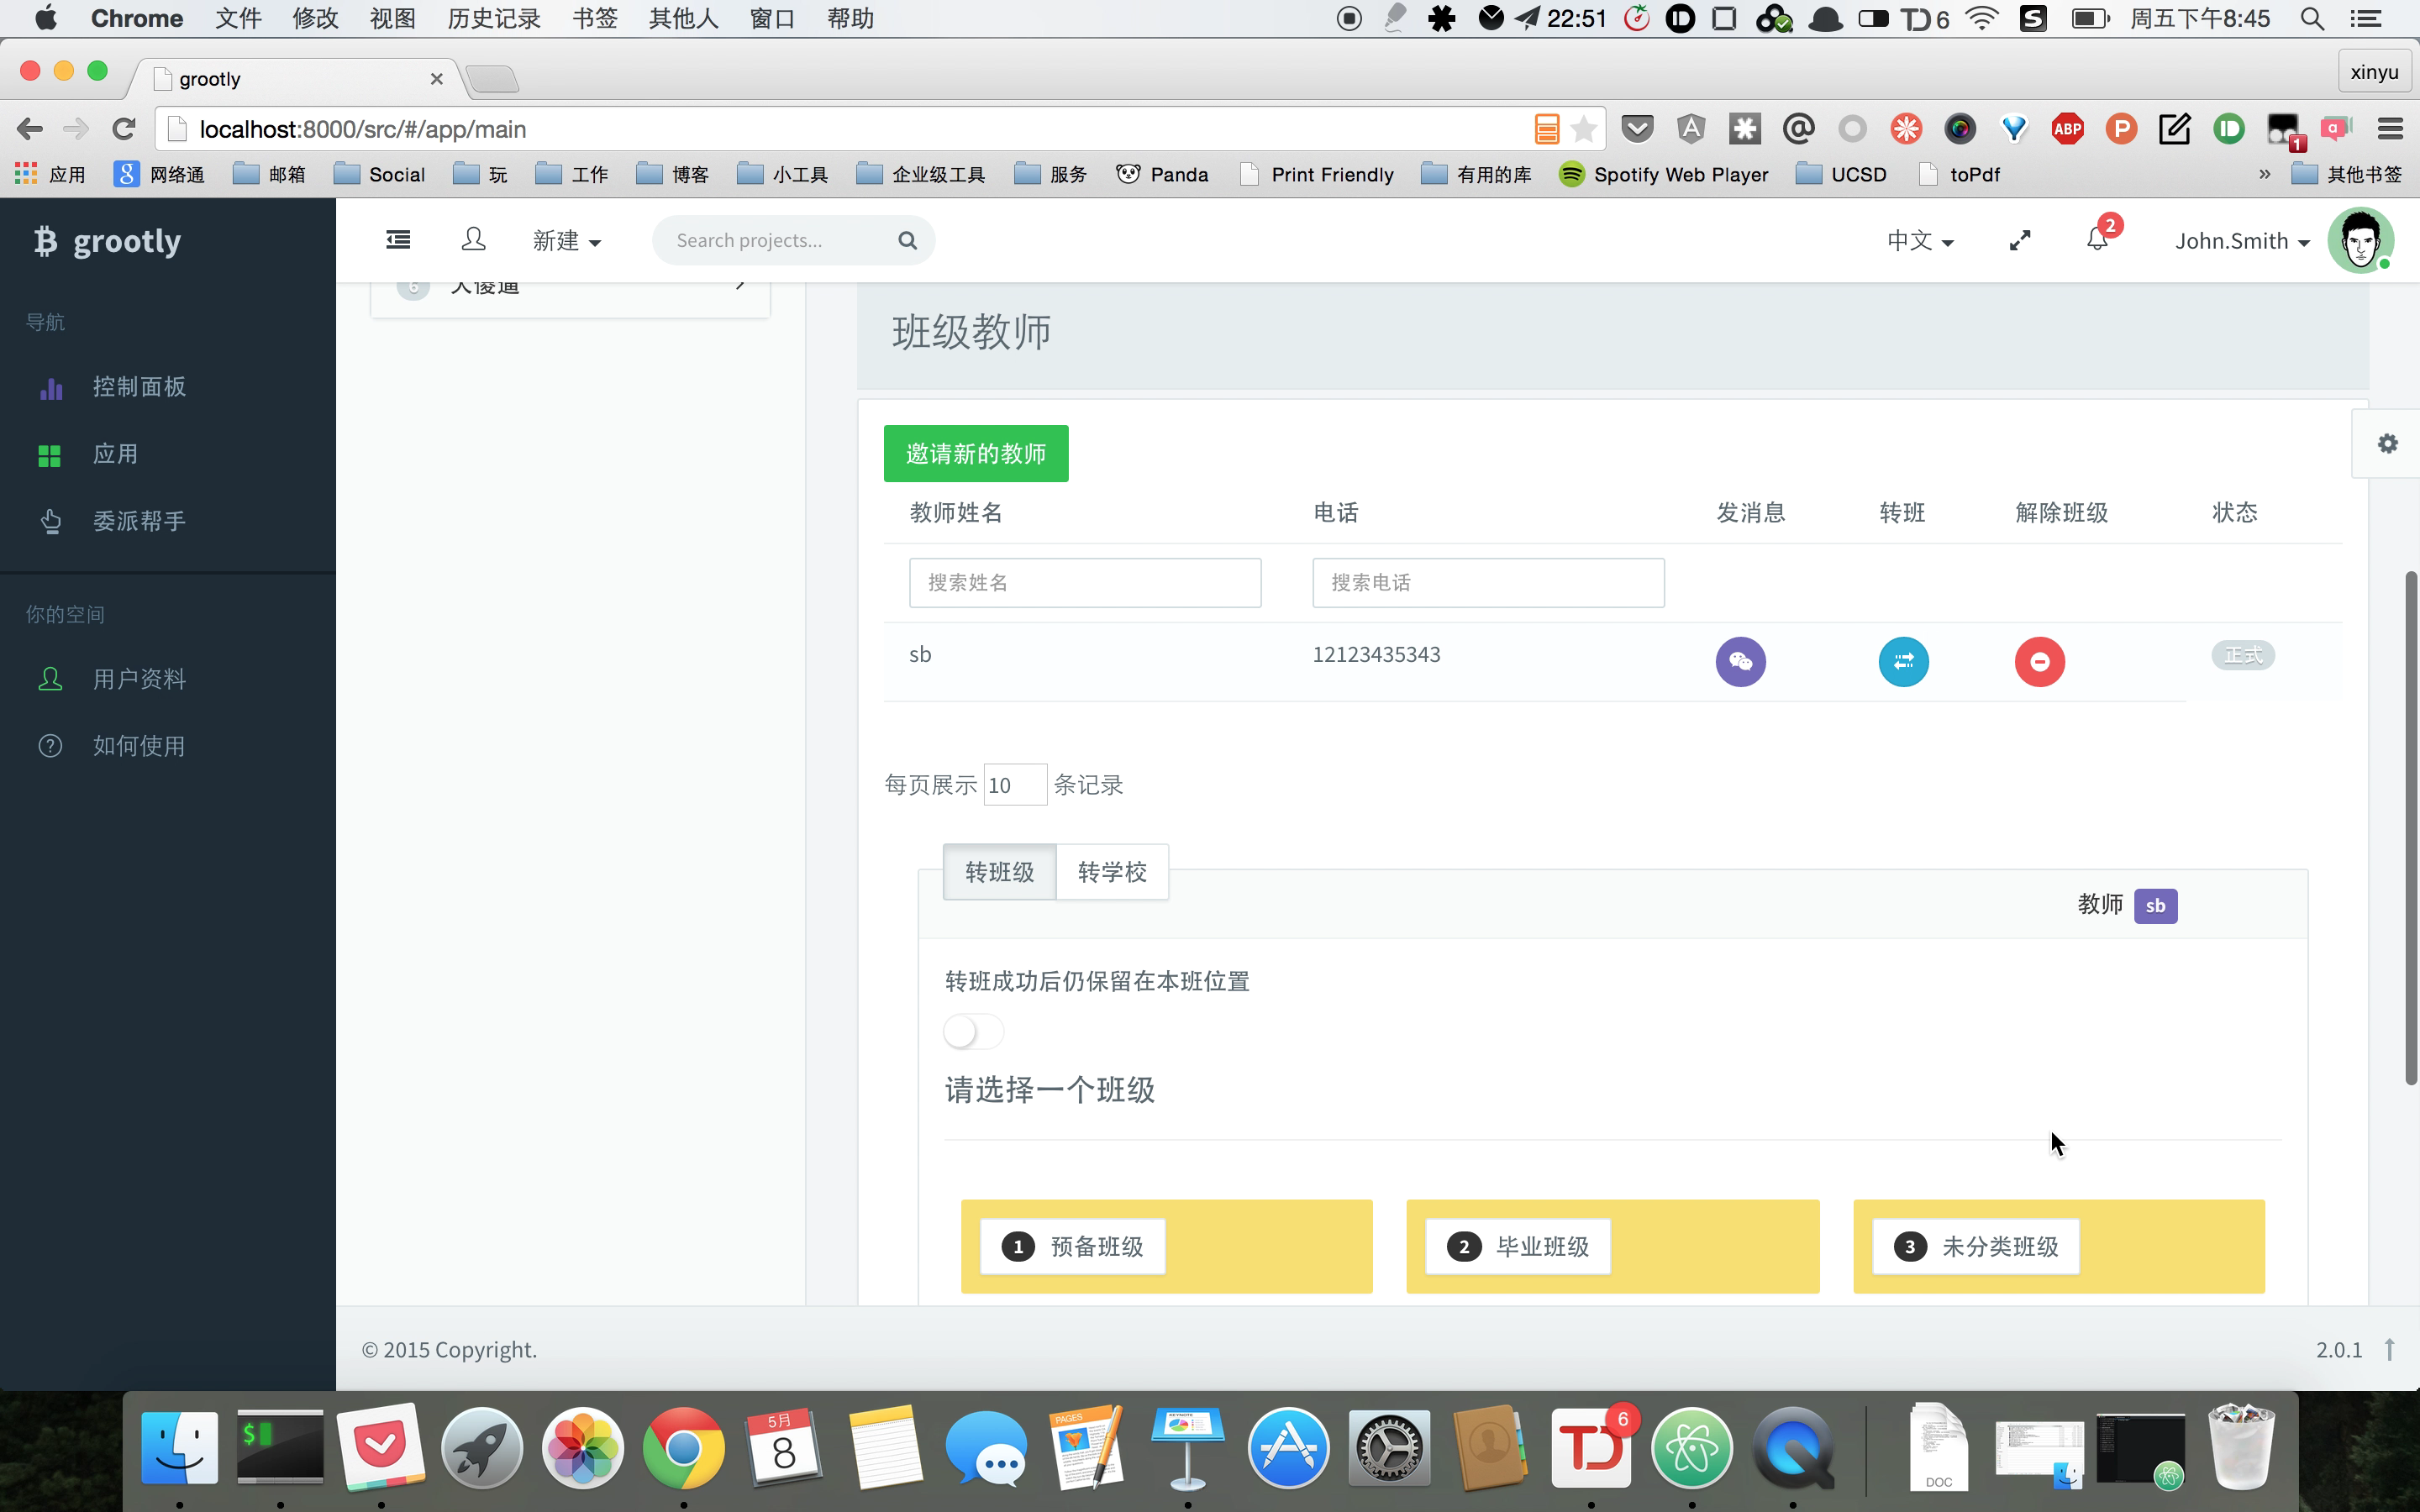
\includegraphics[width=0.7\textwidth]{people_transfer.png}
  \figcaption{Web管理端 人员转班界面}
  \label{fig: pc_people_transfer}
\end{figure}


\item 帮手界面

\begin{figure}[H]
  \centering
  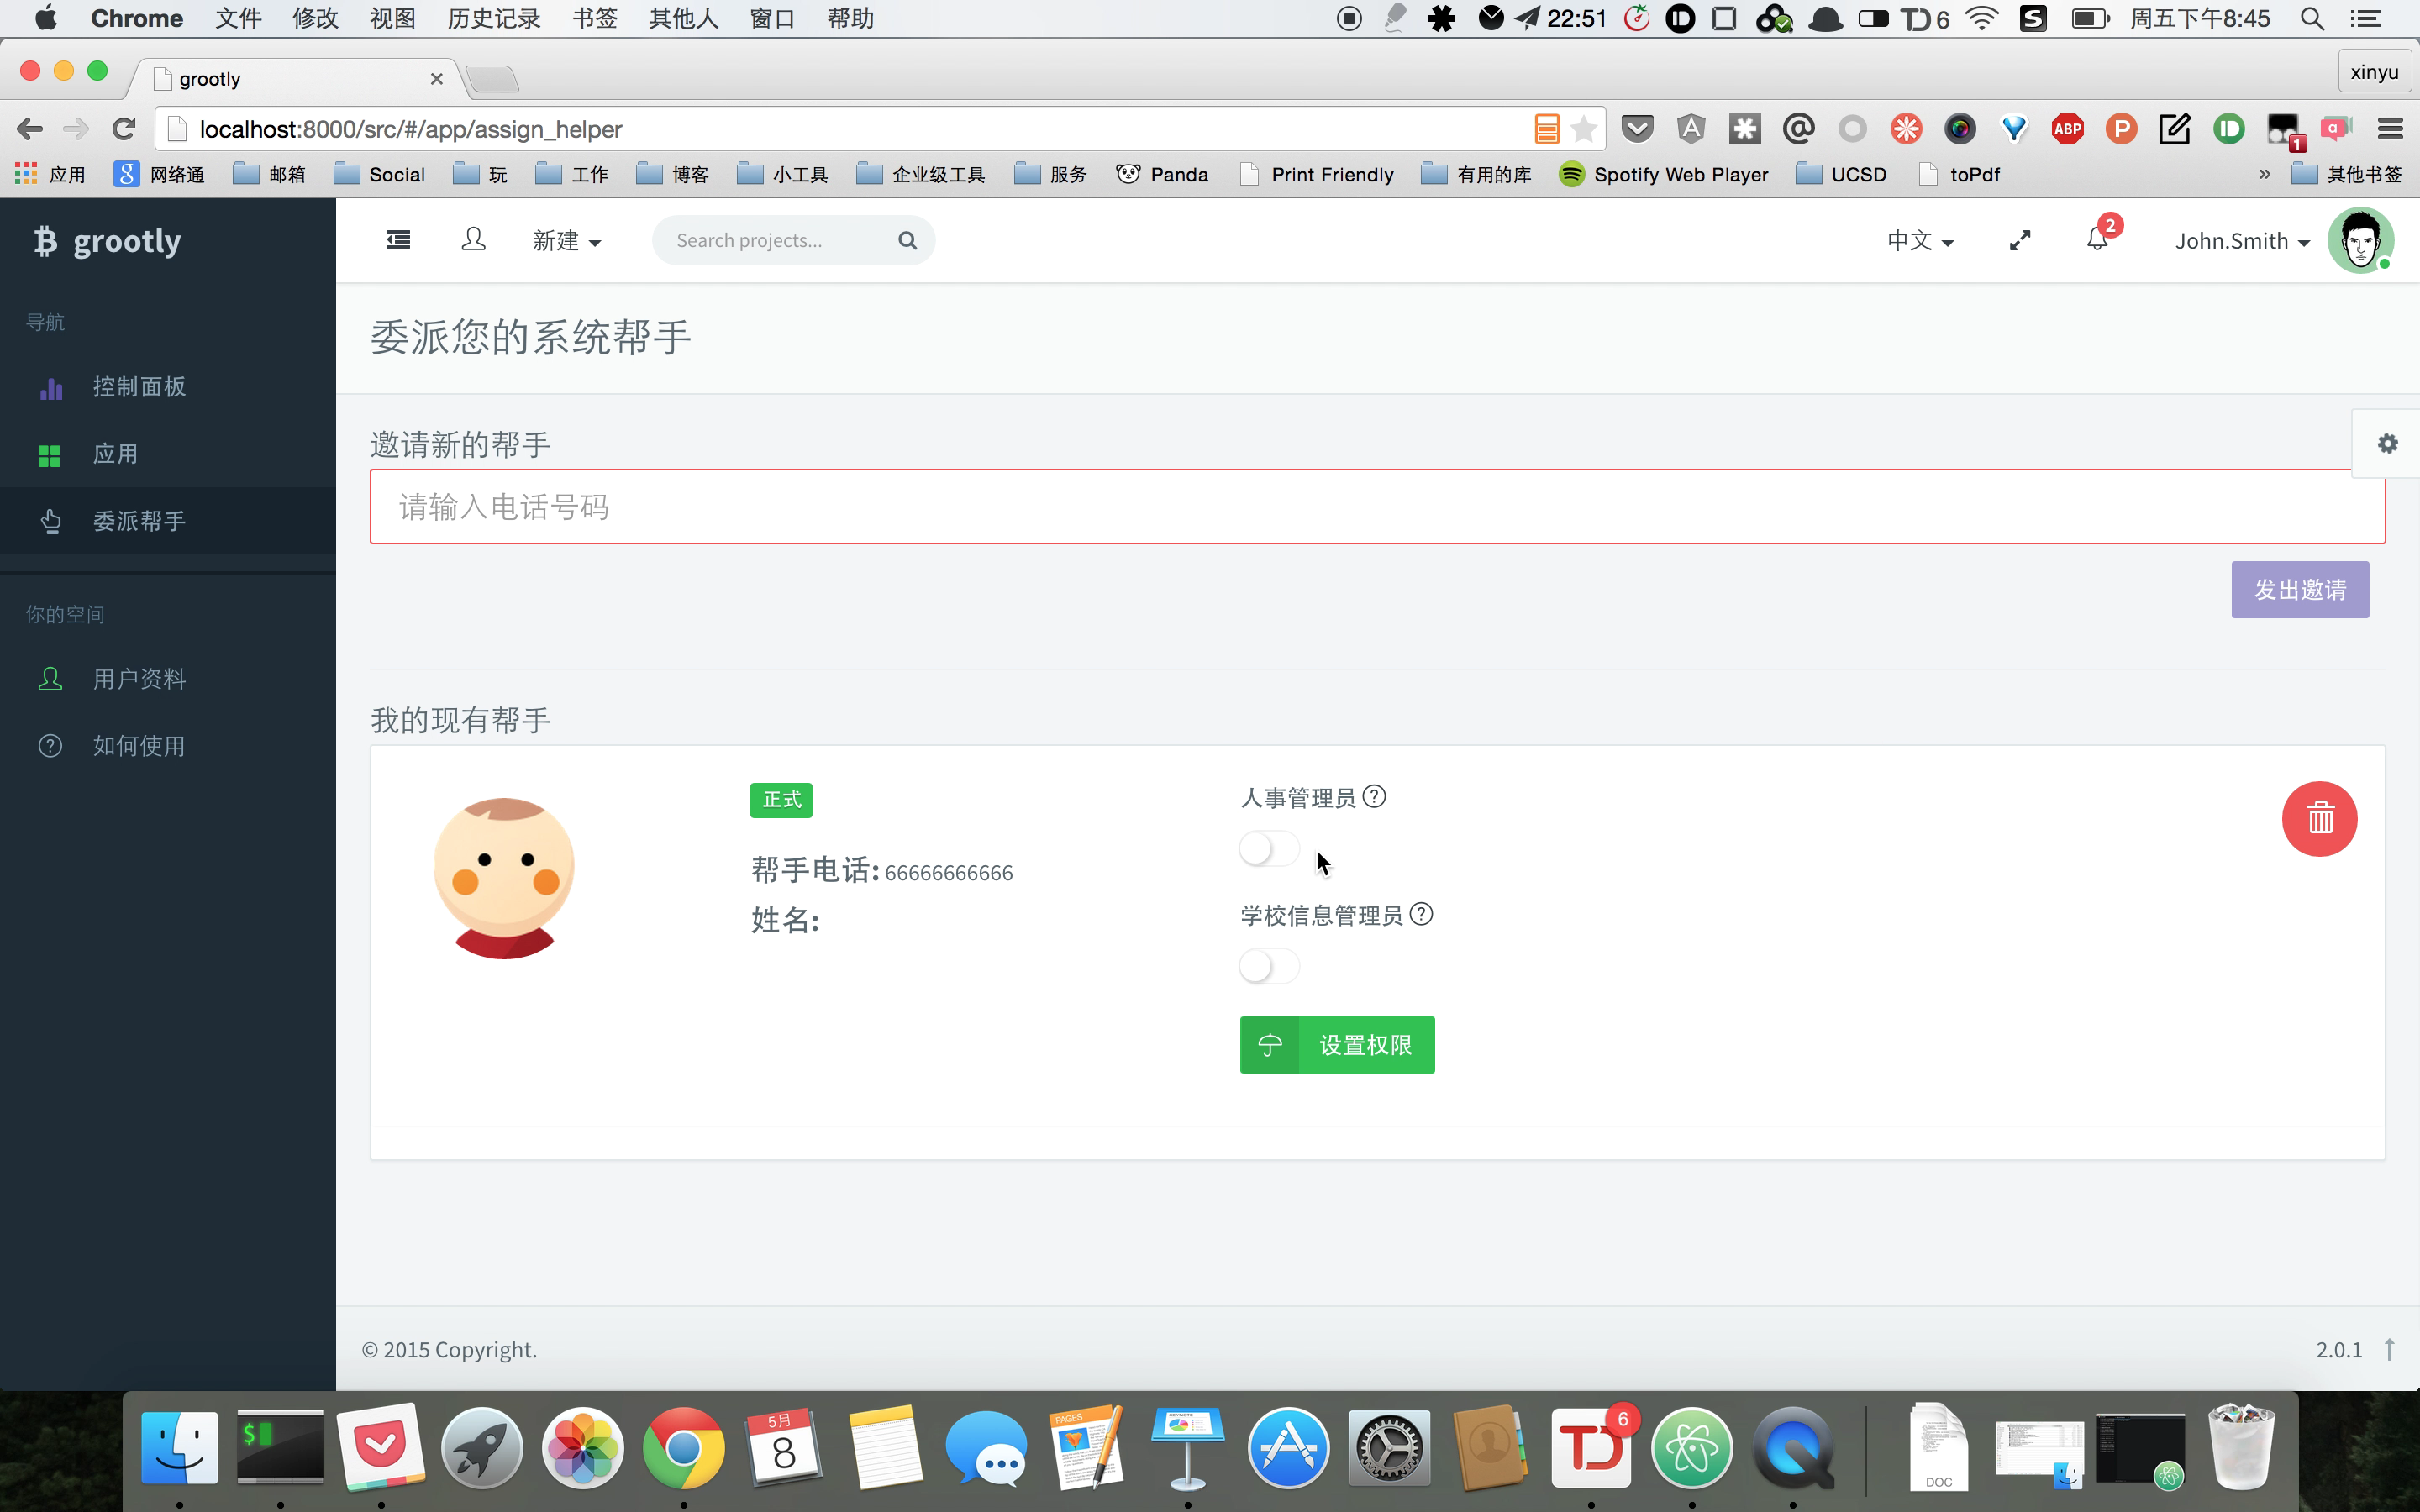
\includegraphics[width=0.7\textwidth]{helper.png}
  \figcaption{Web管理端 帮手界面}
  \label{fig: pc_helper}
\end{figure}


\end{itemize}




\section{Mobile App社交界面设计}

\begin{itemize}

\item 浏览状态界面

\begin{figure}[H]
  \centering
  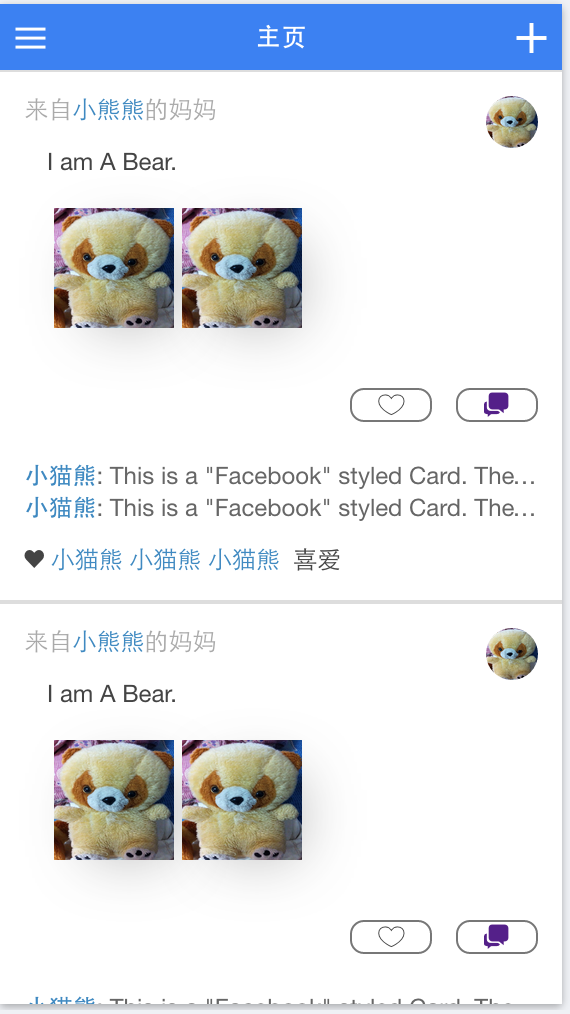
\includegraphics[width=0.3\textwidth]{app_timeline.png}
  \figcaption{App 时间线界面}
  \label{fig: app_timeline}
\end{figure}


\item 发布状态界面

\begin{figure}[H]
  \centering
  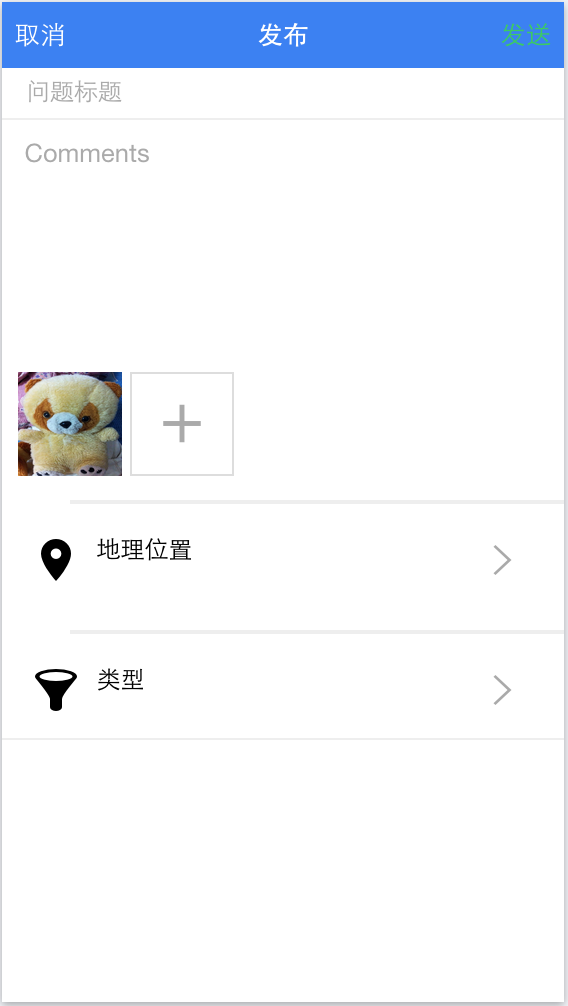
\includegraphics[width=0.3\textwidth]{app_post.png}
  \figcaption{App 发布状态界面}
  \label{fig: app_post}
\end{figure}



\item 聊天界面


\begin{figure}[H]
  \centering
  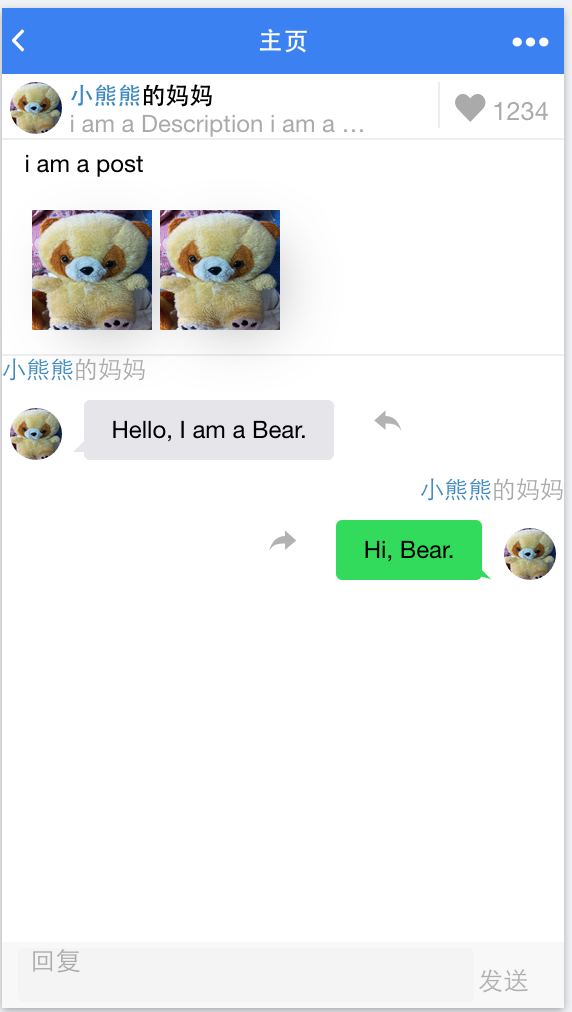
\includegraphics[width=0.3\textwidth]{app_chat.png}
  \figcaption{App 聊天界面}
  \label{fig: app_chat}
\end{figure}


\item 我的班级和学校界面


\begin{figure}[H]
  \centering
  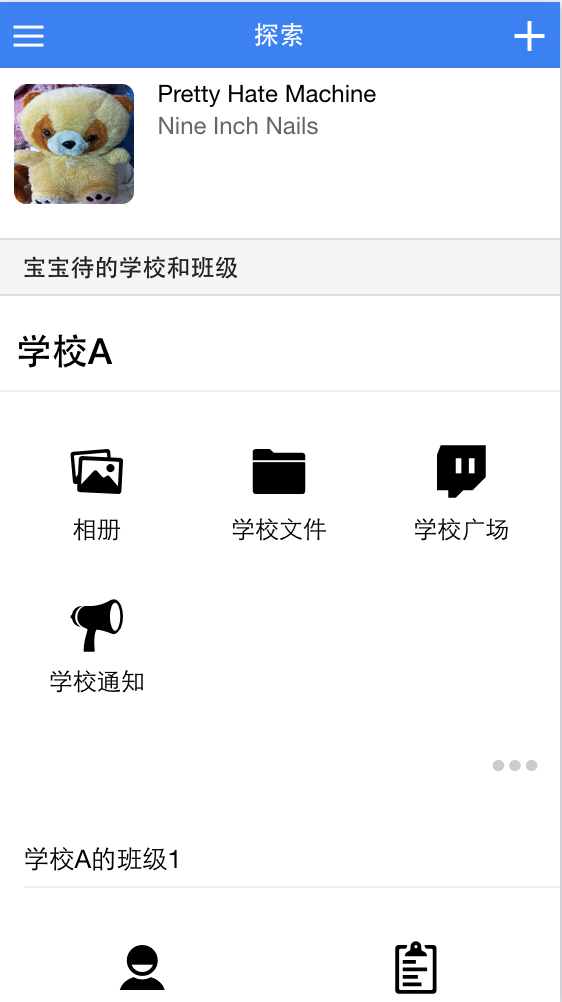
\includegraphics[width=0.3\textwidth]{app_class.png}
  \figcaption{App 我的班级和学校界面}
  \label{fig: app_class}
\end{figure}


\end{itemize}

  \chapter{系统测试}

\section{测试环境和总体方案}

测试方案:


\subsection{系统功能性测试}
  系统的手机端并没有完全完成, 所以功能性测试主要针对于 Web管理端。 功能分为:

  \begin{itemize}
  \item 学校的创建,修改 (删除功能暂时没有实现)
  \item 班级的创建,删除,修改
  \item 网盘,相册操作
  \item 教师,学生的邀请, 转班, 删除
  \item 帮手的邀请,修改,删除
  \end{itemize}

  \textbf{测试环境为}: Mac osx 10.10, Chrome 39

\subsection{系统界面测试}

  分为PC端测试, 和手机端测试

  \textbf{PC端测试环境}:  Mac osx 10.10, Chrome 39

  \textbf{Mobile端测试环境}: iphone5s








\section{系统功能测试}

\subsection{学校的创建,修改}

\begin{table}[H]
  \centering
  \caption{学校的创建}
  \label{tab:1}
  \begin{tabular}{cc}
    \toprule
    测试名称 & 学校的创建  \\

    %%%%%%%%%%%%%%%%%%%%%%%%%%%%%%%%%
    测试人 & 张鑫语 \\
    测试日期 & 2015-05-11 \\

    \midrule
    测试步骤 		& 点击左边Panel的加号, 输入学校数据 \\
    \midrule
    输入数据 		& 学校名: 测试学校, 学校介绍: 测试学校介绍 \\
    预期结果 		& 测试学校被创建 \\
    实际结果             & 与预期结果完全一致 \\
    \bottomrule
  \end{tabular}
\end{table}


\begin{table}[H]
  \centering
  \caption{学校的修改}
  \label{tab:2}
  \begin{tabular}{cc}
    \toprule
    测试名称 & 学校的修改  \\

    %%%%%%%%%%%%%%%%%%%%%%%%%%%%%%%%%
    测试人 & 张鑫语 \\
    测试日期 & 2015-05-11 \\

    \midrule
    测试步骤 		& 点击相关学校, 之后点击详细信息 \\
    \midrule
    输入数据 		&  修改学校名为: 测试学校修改, 学校介绍: 测试学校介绍 \\
    预期结果 		& 测试学校被修改 \\
    实际结果             & 与预期结果完全一致 \\
    \bottomrule
  \end{tabular}
\end{table}


\subsection{班级的创建,修改}

\begin{table}[H]
  \centering
  \caption{班级的创建}
  \label{tab:3}
  \begin{tabular}{cc}
    \toprule
    测试名称 & 班级的创建  \\

    %%%%%%%%%%%%%%%%%%%%%%%%%%%%%%%%%
    测试人 & 张鑫语 \\
    测试日期 & 2015-05-11 \\

    \midrule
    \multirow{2}{*}{测试步骤}
             & 点击测试学校,之后点击右边Panel上的加号 \\
             & 在出现的创建Panel中输入班级数据 \\

    \midrule
    输入数据 		& 班级名: 测试班级, 班级介绍: 测试班级介绍 \\
    预期结果 		& 测试班级被创建 \\
    实际结果             & 与预期结果完全一致 \\
    \bottomrule
  \end{tabular}
\end{table}

\begin{table}[H]
  \centering
  \caption{班级的修改}
  \label{tab:4}
  \begin{tabular}{cc}
    \toprule
    测试名称 & 班级的创建  \\

    %%%%%%%%%%%%%%%%%%%%%%%%%%%%%%%%%
    测试人 & 张鑫语 \\
    测试日期 & 2015-05-11 \\

    \midrule
    \multirow{2}{*}{测试步骤} 		& 点击测试学校,之后点击右边Panel上的加号 \\
    & 在出现的创建Panel中输入班级数据 \\

    \midrule
    输入数据 		& 班级名: 测试班级, 班级介绍: 测试班级介绍 \\
    预期结果 		& 测试班级被创建 \\
    实际结果             & 与预期结果完全一致 \\
    \bottomrule
  \end{tabular}
\end{table}


\subsection{网盘,相册操作}

\begin{table}[H]
  \centering
  \caption{网盘操作}
  \label{tab:5}
  \begin{tabular}{cc}
    \toprule
    测试名称 & 网盘操作  \\

    %%%%%%%%%%%%%%%%%%%%%%%%%%%%%%%%%
    测试人 & 张鑫语 \\
    测试日期 & 2015-05-11 \\

    \midrule
    \multirow{3}{*}{测试步骤} 		& 点击测试学校, 在右边Panel选择文件管理, 之后点击根文件夹 \\
             & 在右下边Panel点击新建, 新建成功后, 修改文件信息并提交 \\
             & 之后点击删除(都在右下部Panel) \\

    \midrule
    输入数据 		& 任意文件 \\
    预期结果 		& 可以在网盘内新建,修改,删除文件 \\
    实际结果             & 与预期结果完全一致 \\
    \bottomrule
  \end{tabular}
\end{table}


\begin{table}[H]
  \centering
  \caption{相册操作}
  \label{tab:6}
  \begin{tabular}{cc}
    \toprule
    测试名称 & 相册操作  \\

    %%%%%%%%%%%%%%%%%%%%%%%%%%%%%%%%%
    测试人 & 张鑫语 \\
    测试日期 & 2015-05-11 \\

    \midrule
    \multirow{3}{*}{测试步骤} 		& 点击测试学校, 在右边Panel选择相册, 在右下边Panel点击上传 \\
             & 上传图片成功后,选中图片并修改信息后提交 \\
             &之后点击右下角红色按钮:删除选中图片 \\

    \midrule
    输入数据 		& 任意图片 \\
    预期结果 		& 可以在相册内新建,修改,删除图片 \\
    实际结果             & 与预期结果完全一致 \\
    \bottomrule
  \end{tabular}
\end{table}


\subsection{教师,学生的邀请,转班,删除}

因为教师和学生管理界面和实现几乎相同, 所以下面统称人员。


\begin{table}[H]
  \centering
  \caption{人员的邀请}
  \label{tab:7}
  \begin{tabular}{cc}
    \toprule
    测试名称 & 人员的邀请  \\

    %%%%%%%%%%%%%%%%%%%%%%%%%%%%%%%%%
    测试人 & 张鑫语 \\
    测试日期 & 2015-05-11 \\

    \midrule
   \multirow{3}{*}{测试步骤} 		& 点击相关学校,在右边班级列表中,点击测试班级 \\
    & 再点击右边Panel中的教师管理, 之后点击右边Panel的邀请新教师 \\
      & 然后输入教师电话 \\
    \midrule
    输入数据 		& 11位数字 \\
    预期结果 		& 教师进入该班级 \\
    实际结果             & 与预期结果完全一致 \\
    \bottomrule
  \end{tabular}
\end{table}

\begin{table}[H]
  \centering
  \caption{人员的转班}
  \label{tab:8}
  \begin{tabular}{cc}
    \toprule
    测试名称 & 人员的转班  \\

    %%%%%%%%%%%%%%%%%%%%%%%%%%%%%%%%%
    测试人 & 张鑫语 \\
    测试日期 & 2015-05-11 \\

    \midrule
    \multirow{3}{*}{测试步骤} 		& 点击相关学校,在右边班级列表中,点击测试班级 \\
             & 再点击右边Panel中的教师管理,在教师列表中选择一个教师\\
             &  点击其右边的 Exchange Icon按钮, 然后选择转向的班级 \\

    \midrule
    输入数据 		& 班级的选择 \\
    预期结果 		& 教师从本班级移入目标班级 \\
    实际结果             & 与预期结果完全一致 \\
    \bottomrule
  \end{tabular}
\end{table}



\begin{table}[H]
  \centering
  \caption{人员的删除}
  \label{tab:9}
  \begin{tabular}{cc}
    \toprule
    测试名称 & 人员的删除  \\

    %%%%%%%%%%%%%%%%%%%%%%%%%%%%%%%%%
    测试人 & 张鑫语 \\
    测试日期 & 2015-05-11 \\

    \midrule
   \multirow{3}{*}{测试步骤} 		& 点击相关学校,在右边班级列表中,点击测试班级 \\
    & 再点击右边Panel中的教师管理,在教师列表中选择一个教师 \\
    & 点击其右边的垃圾箱按钮, 然后点击确定 \\

    \midrule
    输入数据 		& 人员的选择 \\
    预期结果 		& 教师从本班级中移走 \\
    实际结果             & 与预期结果完全一致 \\
    \bottomrule
  \end{tabular}
\end{table}







\subsection{帮手的邀请,修改,删除}


\begin{table}[H]
  \centering
  \caption{帮手邀请}
  \label{tab:11}
  \begin{tabular}{cc}
    \toprule
    测试名称 & 帮手邀请  \\

    %%%%%%%%%%%%%%%%%%%%%%%%%%%%%%%%%
    测试人 & 张鑫语 \\
    测试日期 & 2015-05-11 \\

    \midrule
    \multirow{2}{*}{测试步骤} 		& 点击最左边导航栏中的 “我的帮手”,  \\
                                        & 之后在主界面上部输入电话号码,之后点击 “发出邀请” \\
    \midrule
    输入数据 		& 11位数字 \\
    预期结果 		& 下面帮手列表添加了新的帮手 \\
    实际结果             & 与预期结果完全一致 \\
    \bottomrule
  \end{tabular}
\end{table}


\begin{table}[H]
  \centering
  \caption{帮手修改和删除}
  \label{tab:12}
  \begin{tabular}{cc}
    \toprule
    测试名称 & 帮手修改和删除  \\

    %%%%%%%%%%%%%%%%%%%%%%%%%%%%%%%%%
    测试人 & 张鑫语 \\
    测试日期 & 2015-05-11 \\

    \midrule
    \multirow{3}{*}{测试步骤} 		& 点击最左边导航栏中的 “我的帮手”, \\
             & 之后在主界面中部的帮手列表中, 修改帮手权限 \\
             & 之后点击提交, 然后点击右上角红色垃圾箱按钮。 \\
    \midrule
    输入数据 		& 权限的选择 \\
    预期结果 		& 提交后显示帮手权限被修改,删除后该帮手不出现在列表中 \\
    实际结果             & 与预期结果完全一致 \\
    \bottomrule
  \end{tabular}
\end{table}




\section{系统界面测试}



需要测试的系统界面:

\subsection{电脑端}

\begin{itemize}
\item 学校修改界面
\item 班级界面
\item 班级列表界面
\item 网盘界面
\item 相册界面
\item 教师,学生的管理界面
\item 帮手界面
\end{itemize}

\subsection{手机端}

\begin{itemize}
\item 发布状态界面
\item 浏览状态界面
\item 聊天界面
\item 我的班级和学校界面
\end{itemize}


\subsection{测试结果}

经由第五章的系统界面设计截图, 可以得知系统界面符合设计要求, 操作流畅, 为底层功能提供了比较好的UI接口。 具体截图不在这里冗余。

  \chapter{总结与展望}

\section{总结}


本文介绍了一个幼儿教育领域应用的设计,开发流程和部分实现细节。 从用户的需求, 讲到功能上,架构上的设计, 再讲到实现细节。  在这个过程中, 自己学到了非常多的东西, 感觉意义非凡。



\begin{itemize}
\item 用户需求调研
\item 产品设计
\item UI设计
\item 如何优良架构一个基于Nodejs的大型Web服务
\item 互联网开发团队如何运作
\item 等等...
\end{itemize}


可惜的是, 用户需求调研, 设计流程并没有留下太多的文档。 从设计的角度上说, 其学习价值受到了减弱。 但该应用对于如何实现管理+社交混合系统, 有一定程度上的参考价值。 严格意义上说, 该应用可以被归类为一种垂直领域社交类应用, 也是有效细分市场的体现。


\section{展望}


可以肯定地说,该应用有一定应用前景, 现在自己还没有完全实现, 而且后端和Web前端代码很多东西当时实现的时候由于经验不足, 所以并没有一个比较好的结构, 还需要进行大量的代码重构。 所以未来要做的事情有:

\begin{itemize}
\item  实现手机端的UI交互
\item  重构服务器后端代码
\item  重构Web前端管理功能代码
\item  基于新的后端,实现手机端功能
\end{itemize}

  %自行添加
  %\include{chapter/...}

%%%%%%%%%%%%%%%%%%%%%%%%%%%%%%
%% 附件部分
%%%%%%%%%%%%%%%%%%%%%%%%%%%%%%
\backmatter

  % 参考文献
  % 使用 BibTeX
  % 选择参考文献的排版格式。注意ustcbib这个格式不保证完全符合要求,请自行决定是否使用
  \bibliographystyle{ustcbib}%{GBT7714-2005NLang-UTF8}
  \bibliography{bib/tex}
  \nocite{*} % for every item
  % 不使用 BibTeX
   %%\renewcommand{\baselinestretch}{0.5}
\begin{thebibliography}{10}

\bibitem{deng:01a}
{邓建松,~彭冉冉,~陈长松邓建松,~彭冉冉,~陈长松邓建松,~彭冉冉,~陈长松邓建松,~彭冉冉,~陈长松邓建松,~彭冉冉,~陈长松邓建松,~彭冉冉,~陈长松邓建松,~彭冉冉,~陈长松邓建松,~彭冉冉,~陈长松邓建松,~彭冉冉,~陈长松邓建松,~彭冉冉,~陈长松邓建松,~彭冉冉,~陈长松}.
\newblock {\em \LaTeXe{}~科技排版指南}.
\newblock 科学出版社,~书号:~7-03-009239-2/TP.1516, 北京, 2001.

\bibitem{wang:00a}
王磊.
\newblock {\em \LaTeXe{}~插图指南}.
\newblock 2000.

\bibitem{zhang:03a}
张林波.
\newblock {\em 关于新版~CCT~的说明}.
\newblock 2003.

\bibitem{lshort-cn}
C\TeX{} 翻译小组.
\newblock {\em lshort~中文版~3.20}.
\newblock 2003.

\bibitem{knuth86e}
Donald~E. Knuth.
\newblock {\em Computer Modern Typefaces}, volume~E of {\em Computers and
  Typesetting}.
\newblock Addison-Wesley, Reading, Massachusetts, 1986.

\bibitem{knuth86d}
Donald~E. Knuth.
\newblock {\em {METAFONT}: The Program}, volume~D of {\em Computers and
  Typesetting}.
\newblock Addison-Wesley, Reading, Massachusetts, 1986.

\bibitem{knuth86c}
Donald~E. Knuth.
\newblock {\em The {METAFONT}book}, volume~C of {\em Computers and
  Typesetting}.
\newblock Addison-Wesley, Reading, Massachusetts, 1986.

\bibitem{knuth86b}
Donald~E. Knuth.
\newblock {\em {TeX}: The Program}, volume~B of {\em Computers and
  Typesetting}.
\newblock Addison-Wesley, Reading, Massachusetts, 1986.

\bibitem{knuth86a}
Donald~E. Knuth.
\newblock {\em The {TeX}book}, volume~A of {\em Computers and Typesetting}.
\newblock Addison-Wesley, Reading, Massachusetts, 1986.

\bibitem{lamport85a}
Leslie Lamport.
\newblock {\em {LaTeX} --- A Document Preparation System: User's Guide and
  Reference Manual}.
\newblock Addison-Wesley, Reading, Massachusetts, 2nd edition, 1985.

\end{thebibliography}


  % 附录,没有请注释掉
  \begin{appendix}
    
\chapter{关于硕士、博士学位论文撰写要求}
\label{chap:requires}

学位论文是学位申请者为申请学位而撰写的学术论文,它集中作者在研究工作中获得可行的发明、理论和见解,是评判学位申请人学术水平的重要依据和获得学位的必要条件之一,也是科研领域中的主要文献资料和社会宝贵财富。
为提高研究生学位论文的质量,做到学位论文在内容和格式上规范化与统一化,特作如下规定:

\section{对学位论文的基本要求}

\textbf{一下文字仅作示例,一切以学校规定为准!}

\subsection{硕士学位论文}

根据《中华人民共和国学位条例暂行实施办法》第八条的规定,硕士学位论文应能表明作者确已在本门学科上掌握了坚实的基础理论和系统的专门知识,并对所研究的课题有新的见解,有从事科学研究或独立担负专门技术工作的能力。硕士学位论文工作一般是在硕士生完成培养计划规定的课程学习后开始,其工作内容因学科的性质不同而有所差异,一般包括文献阅读、开题报告、拟定并实施工作计划、科研调查、实验研究、理论分析和文字总结等工作。论文正文一般应不少于3万字。硕士学位论文必须有一定的工作量,在论文题目确定后,用于论文工作的时间一般不应少于1.5年。

\subsection{博士学位论文}

根据《中华人民共和国学位条例暂行实施办法》第十三条的规定,博士学位论文应能表明作者确已在本门学科上掌握了坚实宽广的基础理论和系统深入的专门知识,具有独立从事科学研究工作的能力,并在科学或专门技术工作上做出了创造性的成果。博士学位论文工作是攻读博士学位研究生培养的最重要环节,其工作时间一般应不少于2学年。博士生入学后在导师指导下明确科研方向,收集资料,阅读文献,进行调查研究,确定研究课题。一般在第二至第三学期通过开题报告并制定论文工作计划。博士生应根据论文工作计划分阶段在教研室、学术会议上报告科研和论文工作的进展情况。论文正文一般应不少于5万字。博士生用于论文研究和撰写学位论文的时间一般应不得少于2年。

特别应注意,学位论文应是本人的研究成果,在导师指导下独立完成,不得抄袭或剽窃他人成果。论文应反映作者较好地掌握了本学科、专业的研究方法和技能,学术观点必须言之有理、持之有据,论文内容应层次分明,数据可靠,文字简炼,推理严谨,立论正确。

\section{对学位论文的格式要求}

\subsection{编写要求}

硕士、博士学位论文一般应由以下全部或某几部分组成,依次为:封面、中文摘要、英文摘要 、目录、符号说明、正文、参考文献、附录、附图表、致谢、攻读学位期间发表的学术论文目录。

具体要求如下:

\subsubsection{封面}

采用研究生院规定的统一封面,封面上填写论文题目、作者姓名、导师姓名、学科(专业) 、论文完成时间。上述内容也应在扉页上填写清楚。论文题目采用黑体26磅加粗居中,其他采用宋体16磅居中。书脊用黑体12磅,上方写论文题目,中间写系别,下方写研究生姓名(彩色封面在制信厂或印刷厂装订)。

\subsubsection{论文摘要}

学位论文的中文摘要应以最简洁的语言介绍论文的概要、作者的突出论点、新见解或创造性成果。硕士学位论文中文摘要一般应在500字左右,博士学位论文中文摘要一般在1500字左右。英文摘要(Abstract)内容应与中文摘要基本相对应,要语句通顺,语法正确,能正确概括文章的内容。摘要标题采用黑体16磅居中,正文采用宋体12磅(英文用Times New Roman体12磅),行距20磅。

\subsubsection{正文}

正文是学位论文的主体和核心部分,它是将学习、研究和调查过程中筛选、观察和测试所获得的材料,经过加工整理和分析研究,由材料而形成论点。不同学科、专业有着不同的写作内容,但作为一般要求,论据、论点应力求准确、完备、清晰、通顺,实事求是,客观真切,简短精炼,合乎逻辑。一般标题字体采用黑体14磅,多级标题可采用粗体14磅或粗体12磅。正文字体采用宋体12磅(英文用Times New Roman体12磅),两端对齐书写,行距20磅。


绪论或引言是学位论文主体部分的开端,主要说明研究工作的缘起、沿革、目的、涉及范围 、国内外研究现状、相关领域的前人研究成果和知识空白、理论分析的依据、研究设想、研究方法和实际设计的概述,以及文中拟解决的问题、理论意义和实用价值等,应言简意赅,不要与摘要雷同或成为摘要的解释,也不是提要。

结论是学位论文最终和总体的结论,是整篇论文的归宿,应明确、精炼、完整、准确。要着重阐述作者研究的创造性成果、新见解、新发现和新发展,及其在本研究领域中的地位、作用、价值和意义,还可进一步提出需要讨论的问题和建议。学位论文中的计量单位、制图、制表、公式规范、缩略词和符号必须遵循GB 3100~3102—93(国家技术监督局1993-12-27发布,1994-07-01实施)有关量和单位的规定。如无标准可循,应采用本学科或专业有关权威性机构或学术团体所公布的规定。如不得已必需引用某些未公知公用的、不易为同行读者所理解的或系作者自行拟定的符合、记号、缩略词等,均应一一在第一次出现时加以说明,给以明确的定义。

\subsubsection{参考文献}

参考文献应按文中引用的顺序列出,可以分列在各章末尾,也可以列在正文的末尾。

本着以严谨求实的科学态度撰写论文,凡学位论文中有引用他人成果之处,均应详细列出所引文献的名称、作者、发表刊物、发表时间、卷号、页码等。标题字体采用黑体14磅,正文字体采用宋体10磅(英文用Times New Roman体10磅),行距16磅。

\subsubsection{附录}
主要列入正文内过分冗长的公式推导,供查读方便所需的辅助性数学工具或表格,重复性数据图表,论文使用的缩写,程序全文及说明等。

\subsubsection{致谢}

表达作者对完成论文和学业提供帮助的老师、同学、领导、同事及亲属的感激之情。

\subsubsection{攻读学位期间发表的学术论文目录}

按学术论文发表的时间顺序,列齐本人在攻读学位期间发表或已录用的学术论文清单(发表刊物名称、卷册号、页码、年月及论文署名、作者排序)。

\subsection{打印}

按照有关规定,凡授予中华人民共和国学位者,学位论文必须用中文撰写,同时一律用A4标准纸打印输出,一般应有篇眉。篇眉和页码均采用宋体10磅居中,页面设置上边距3.8cm、下边距为3.0cm,左边距为3.5cm、右边距为3.0cm。

\subsection{装订}

学位论文撰写完成后,用研究生院统一封面线装订成册。所需份数由研究生本人及导师掌握(可参考学位申请上报材料清单的要求)。

  \end{appendix}

  \makeatletter
  \ifustc@bachelor
  	
\begin{thanks}

感谢原本科模板的作者XPS、硕博模板的作者刘青松以及它们的维护者的辛勤工作!

感谢大家对本模板更新工作的支持!

本模板以及本示例文档还存在许多不足之处,欢迎大家测试并及时提供反馈。

\begin{flushright}
ywg@USTC
\end{flushright}


在中国科技大学完成本科和硕博连读学业的九年里,我所从事的学习和研究工作,都是在导师以及系里其他老师和同学的指导和帮助下进行的。在完成论文之际,请容许我对他们表达诚挚的谢意。

首先感谢导师XXX教授和XXX副教授多年的指导和教诲,是他们把我带到了计算机视觉的研究领域。X老师严谨的研究态度及忘我的工作精神,X老师认真细致的治学态度及宽广的胸怀,都将使我受益终身。

感谢班主任XXX老师和XX老师多年的关怀。感谢XXX、XX、XX等老师,他们本科及研究生阶段的指导给我研究生阶段的研究工作打下了基础。

感谢XX、XXX、XXX、XX、XXX、XXX、XXX、XX等师兄师姐们的指点和照顾;感谢XXX、XX、XXX等几位同班同学,与你们的讨论使我受益良多;感谢XXX、XX、XXX、XX、XXX等师弟师妹,我们在XXX实验室共同学习共同生活,一起走过了这段愉快而难忘的岁月。

感谢科大,感谢一路走过来的兄弟姐妹们,在最宝贵年华里,是你们伴随着我的成长。

最后,感谢我家人一贯的鼓励和支持,你们是我追求学业的坚强后盾。

\vskip 18pt

\begin{flushright}

~~~~赵钱孙~~~~

\today

\end{flushright}

\end{thanks}
%硕博致谢部分
  \else
    % 致谢
    %	
\begin{thanks}

感谢原本科模板的作者XPS、硕博模板的作者刘青松以及它们的维护者的辛勤工作!

感谢大家对本模板更新工作的支持!

本模板以及本示例文档还存在许多不足之处,欢迎大家测试并及时提供反馈。

\begin{flushright}
ywg@USTC
\end{flushright}


在中国科技大学完成本科和硕博连读学业的九年里,我所从事的学习和研究工作,都是在导师以及系里其他老师和同学的指导和帮助下进行的。在完成论文之际,请容许我对他们表达诚挚的谢意。

首先感谢导师XXX教授和XXX副教授多年的指导和教诲,是他们把我带到了计算机视觉的研究领域。X老师严谨的研究态度及忘我的工作精神,X老师认真细致的治学态度及宽广的胸怀,都将使我受益终身。

感谢班主任XXX老师和XX老师多年的关怀。感谢XXX、XX、XX等老师,他们本科及研究生阶段的指导给我研究生阶段的研究工作打下了基础。

感谢XX、XXX、XXX、XX、XXX、XXX、XXX、XX等师兄师姐们的指点和照顾;感谢XXX、XX、XXX等几位同班同学,与你们的讨论使我受益良多;感谢XXX、XX、XXX、XX、XXX等师弟师妹,我们在XXX实验室共同学习共同生活,一起走过了这段愉快而难忘的岁月。

感谢科大,感谢一路走过来的兄弟姐妹们,在最宝贵年华里,是你们伴随着我的成长。

最后,感谢我家人一贯的鼓励和支持,你们是我追求学业的坚强后盾。

\vskip 18pt

\begin{flushright}

~~~~赵钱孙~~~~

\today

\end{flushright}

\end{thanks}
%硕博致谢部分\dfrac{分子}{分母}
    % 发表文章目录
  %  
\chapter{在读期间发表的学术论文与取得的研究成果}

\noindent\textbf{研究工作:}

\begin{enumerate}

\item A A A A A A A A A
\item A A A A A A A A A
\item A A A A A A A A A
\item A A A A A A A A A

\end{enumerate}


\noindent\textbf{已发表论文:}

\begin{enumerate}

\item A A A A A A A A A 
\item A A A A A A A A A
\item A A A A A A A A A
\item A A A A A A A A A
\item A A A A A A A A A
\item A A A A A A A A A
\item A A A A A A A A A
\item A A A A A A A A A

\end{enumerate}

\vskip 1cm

\noindent\textbf{待发表论文:}

\begin{enumerate}

\item A A A A A A A A A

\end{enumerate} 
  \fi
  \makeatother

\end{document}
